\documentclass[11pt,a4paper]{article}
\usepackage[margin=23mm]{geometry}
\usepackage[T1]{fontenc}
\usepackage{lmodern,microtype,amsmath,amssymb,booktabs,longtable,array,graphicx,float}
\usepackage[round,authoryear]{natbib}
\usepackage[dvipsnames]{xcolor}
\usepackage[colorlinks=true,linkcolor=MidnightBlue,citecolor=MidnightBlue,urlcolor=MidnightBlue]{hyperref}
\usepackage{caption,fancyhdr}
\captionsetup{font=small,labelfont=bf}
\setlength{\headheight}{14pt}\setlength{\parskip}{4pt}\setlength{\parindent}{0pt}\setlength{\emergencystretch}{2em}
\setcounter{topnumber}{3}\renewcommand{\topfraction}{.92}\renewcommand{\textfraction}{.07}
\pagestyle{fancy}\fancyhf{}\lhead{PAT16: exploratory longitudinal connectomics}\rhead{18 October 2026}\cfoot{\thepage}
\newcommand{\LesionVolume}{45.431}
\newcommand{\CommonNodes}{100}
\newcommand{\CantabCount}{28}
\newcommand{\AssessmentCount}{47}
\newcommand{\JointPrimaryMedian}{-0.04050}
\newcommand{\JointPrimaryLow}{-0.08390}
\newcommand{\JointPrimaryHigh}{+0.01584}
\newcommand{\JointPrimarySCShare}{1.48}
\newcommand{\JointPrimaryFCShare}{98.21}
\newcommand{\JointPrimaryInteractionShare}{0.30}
\newcommand{\JointPrimaryPositive}{9.16}
\newcommand{\JointPrimaryReselectMedian}{-0.04438}
\newcommand{\JointPrimaryReselectLow}{-0.09294}
\newcommand{\JointPrimaryReselectHigh}{+0.01377}
\newcommand{\JointPrimaryReselectSCShare}{10.82}
\newcommand{\JointPrimaryReselectFCShare}{84.22}
\newcommand{\JointPrimaryReselectInteractionShare}{4.96}
\newcommand{\JointPrimaryReselectPositive}{6.84}
\newcommand{\JointStrictMedian}{-0.02981}
\newcommand{\JointStrictLow}{-0.08436}
\newcommand{\JointStrictHigh}{+0.03146}
\newcommand{\JointStrictSCShare}{1.50}
\newcommand{\JointStrictFCShare}{98.18}
\newcommand{\JointStrictInteractionShare}{0.31}
\newcommand{\JointStrictPositive}{17.49}
\newcommand{\JointStrictReselectMedian}{-0.02570}
\newcommand{\JointStrictReselectLow}{-0.08510}
\newcommand{\JointStrictReselectHigh}{+0.03905}
\newcommand{\JointStrictReselectSCShare}{15.23}
\newcommand{\JointStrictReselectFCShare}{79.89}
\newcommand{\JointStrictReselectInteractionShare}{4.88}
\newcommand{\JointStrictReselectPositive}{21.61}
\newcommand{\JointStrictMotionMedian}{-0.04874}
\newcommand{\JointStrictMotionLow}{-0.09073}
\newcommand{\JointStrictMotionHigh}{-0.01323}
\newcommand{\JointStrictMotionSCShare}{4.10}
\newcommand{\JointStrictMotionFCShare}{95.39}
\newcommand{\JointStrictMotionInteractionShare}{0.51}
\newcommand{\JointStrictMotionPositive}{0.20}
\newcommand{\JointStrictMotionReselectMedian}{-0.04638}
\newcommand{\JointStrictMotionReselectLow}{-0.09394}
\newcommand{\JointStrictMotionReselectHigh}{-0.00091}
\newcommand{\JointStrictMotionReselectSCShare}{31.81}
\newcommand{\JointStrictMotionReselectFCShare}{62.56}
\newcommand{\JointStrictMotionReselectInteractionShare}{5.63}
\newcommand{\JointStrictMotionReselectPositive}{2.29}
\newcommand{\JointStrictHalfMedian}{-0.02208}
\newcommand{\JointStrictHalfLow}{-0.05720}
\newcommand{\JointStrictHalfHigh}{+0.01065}
\newcommand{\JointStrictHalfSCShare}{5.56}
\newcommand{\JointStrictHalfFCShare}{93.94}
\newcommand{\JointStrictHalfInteractionShare}{0.50}
\newcommand{\JointStrictHalfPositive}{9.37}
\newcommand{\JointStrictHalfReselectMedian}{-0.01886}
\newcommand{\JointStrictHalfReselectLow}{-0.06051}
\newcommand{\JointStrictHalfReselectHigh}{+0.02351}
\newcommand{\JointStrictHalfReselectSCShare}{37.36}
\newcommand{\JointStrictHalfReselectFCShare}{57.22}
\newcommand{\JointStrictHalfReselectInteractionShare}{5.42}
\newcommand{\JointStrictHalfReselectPositive}{19.23}
\newcommand{\JointTailHalfMin}{-0.00233}
\newcommand{\JointTailHalfMax}{+0.00047}
\newcommand{\JointSupportLow}{814.5}
\newcommand{\JointSupportMedian}{826.0}
\newcommand{\JointSupportHigh}{840.0}
\newcommand{\JointJaccardLow}{0.8970}
\newcommand{\JointJaccardMedian}{0.9188}
\newcommand{\JointJaccardHigh}{0.9406}
\newcommand{\PreAnatFC}{0.087}
\newcommand{\PreAnatCoupling}{0.188}
\newcommand{\PreAnatFCOld}{0.100}
\newcommand{\PreAnatCouplingOld}{0.184}
\newcommand{\PreLegacyFC}{0.360}
\newcommand{\PreLegacyCoupling}{0.147}
\newcommand{\PreConsensusEdges}{1160}
\newcommand{\PreStreamlines}{26488}
\newcommand{\PreAssigned}{16258}
\newcommand{\PreFrames}{146}
\newcommand{\PreMinutes}{5.84}
\newcommand{\PreDof}{107}
\newcommand{\PreCoupling}{0.188}
\newcommand{\PostAnatFC}{0.046}
\newcommand{\PostAnatCoupling}{0.146}
\newcommand{\PostAnatFCOld}{0.048}
\newcommand{\PostAnatCouplingOld}{0.146}
\newcommand{\PostLegacyFC}{0.133}
\newcommand{\PostLegacyCoupling}{0.142}
\newcommand{\PostConsensusEdges}{1163}
\newcommand{\PostStreamlines}{26421}
\newcommand{\PostAssigned}{15889}
\newcommand{\PostFrames}{150}
\newcommand{\PostMinutes}{6}
\newcommand{\PostDof}{111}
\newcommand{\PostCoupling}{0.146}
\newcommand{\PreSCComponents}{1}
\newcommand{\PreSCBinaryE}{0.5687}
\newcommand{\PreSCWeightedE}{0.04806}
\newcommand{\PreFCWeightedE}{0.2136}
\newcommand{\PreMeanFCPrimary}{0.087}
\newcommand{\PreMeanFCStrict}{0.108}
\newcommand{\PreMeanFCGSR}{0.0026}
\newcommand{\PreMeanFCOld}{0.100}
\newcommand{\PreCouplingOld}{0.184}
\newcommand{\PreMeanFCAlt}{0.089}
\newcommand{\PreCouplingAlt}{0.186}
\newcommand{\PreAssignedTwo}{9544}
\newcommand{\PreAssignedEight}{18204}
\newcommand{\PreSomMotZ}{0.265}
\newcommand{\PreControlZ}{0.253}
\newcommand{\PostSCComponents}{1}
\newcommand{\PostSCBinaryE}{0.5713}
\newcommand{\PostSCWeightedE}{0.04512}
\newcommand{\PostFCWeightedE}{0.1936}
\newcommand{\PostMeanFCPrimary}{0.046}
\newcommand{\PostMeanFCStrict}{0.041}
\newcommand{\PostMeanFCGSR}{-0.0002}
\newcommand{\PostMeanFCOld}{0.048}
\newcommand{\PostCouplingOld}{0.146}
\newcommand{\PostMeanFCAlt}{0.044}
\newcommand{\PostCouplingAlt}{0.145}
\newcommand{\PostAssignedTwo}{10332}
\newcommand{\PostAssignedEight}{17918}
\newcommand{\PostSomMotZ}{0.149}
\newcommand{\PostControlZ}{0.243}
\newcommand{\SCWeightedPercentChange}{-6.1}
\newcommand{\PrimarySCDelta}{-0.04173}
\newcommand{\StrictSCDelta}{-0.03424}
\newcommand{\PreStrictCoupling}{0.161}
\newcommand{\PostStrictCoupling}{0.127}
\newcommand{\RefitFrozenMedian}{-0.04050}
\newcommand{\RefitFrozenLow}{-0.08390}
\newcommand{\RefitFrozenHigh}{+0.01584}
\newcommand{\RefitFrozenPositive}{9.16}
\newcommand{\RefitFrozenFCShare}{98.21}
\newcommand{\RefitCoefficientsMedian}{-0.04364}
\newcommand{\RefitCoefficientsLow}{-0.09795}
\newcommand{\RefitCoefficientsHigh}{+0.03636}
\newcommand{\RefitCoefficientsPositive}{11.75}
\newcommand{\RefitCoefficientsFCShare}{98.95}
\newcommand{\RefitFullMedian}{-0.02069}
\newcommand{\RefitFullLow}{-0.09189}
\newcommand{\RefitFullHigh}{+0.05442}
\newcommand{\RefitFullPositive}{32.13}
\newcommand{\RefitFullFCShare}{99.11}
\newcommand{\PrimaryFCMedian}{-0.04694}
\newcommand{\PrimaryFCLow}{-0.10261}
\newcommand{\PrimaryFCHigh}{+0.00832}
\newcommand{\PrimaryFCShare}{98.33}
\newcommand{\PrimarySCShare}{1.18}
\newcommand{\PrimaryInteractionShare}{0.49}
\graphicspath{{figures/}}
\title{From a local glioma to distributed brain networks:\\a reproducible, exploratory longitudinal case study of PAT16}
\author{Research draft prepared for Arvid Lundervold\\\small Computational analysis assisted by Codex; authorship and clinical review pending}
\date{18 October 2026}
\begin{document}\maketitle
\begin{abstract}
A local tumour-growth model alone cannot describe the distributed functions affected by glioma and its treatment. We built a self-contained Python study linking structural MRI, diffusion MRI, resting-state fMRI and pre/postoperative cognitive and psychosocial assessments in sub-PAT16. A common 100-parcel cortical atlas supports reconstructed structural connectivity (SC) and functional connectivity (FC). We recommend session-specific 16/20 seed-repeat consensus support, weighted by the all-run mean count per 10,000 attempted seeds. Structural graphs retain \PreConsensusEdges{}/\PostConsensusEdges{} edges; primary longitudinal coupling uses their fixed 823-edge intersection with session-specific weights. We recommend five PCs from session-specific anatomical WM/CSF cores, with temporal preprocessing, scaling and PCA fitted only on retained frames, plus joint motion/trend/DCT regression. This post hoc methodological choice replaces historical noncortical PCA in the main analyses; all other denoising models remain sensitivities. Primary FC retained \PreFrames{}/\PostFrames{} frames and \PreDof{}/\PostDof{} residual degrees of freedom. Mean FC was \PreMeanFCPrimary{}/\PostMeanFCPrimary{} and SC--FC coupling \PreCoupling{}/\PostCoupling{} pre/post. At 20\% density, weighted SC efficiency was \PreSCWeightedE{}/\PostSCWeightedE{}. Anatomical regression reduces processing dependence but removes about 90\% of cortical-mean residual variance, which can include neural signal. Component count remains consequential. We recommend 200 nonreplacement block subsets, each containing 97 distinct eligible frames per session, with the complete WM/CSF nuisance estimator refitted and crossed with 500 whole-run SC draws on fixed support. The observed coupling change remains $-0.04173$; subset median change is $\PrimaryFCMedian{}$ with conditional 2.5/97.5-percentile range $[\PrimaryFCLow{},\PrimaryFCHigh{}]$. These are stability ranges for shorter-sample estimators, not full-run confidence intervals. FC contributes \PrimaryFCShare{}\% of conditional grid variance. The two-thirds common-duration rule is a post hoc engineering compromise specified before its new contrasts, not an optimality or coverage result. Frozen fits, repeated-row bootstraps, block lengths, retained fractions and motion matching remain sensitivities. Factorial controls identify PCA-loading refits under repeated-frame weights as a major recentering mechanism. Matched 68-frame analyses identify interacting frame selection, nuisance refitting and SC-support dependence; the coupling-change direction remains unresolved. In the historical single-run sensitivity, pre-op-only edges dominate signed rank accounting, with distributed network contributions and substantial cancellation. Repeated tractography shows unstable low-count/session-specific support; count and consensus cutoffs further change the coupling contrast. Simple reaction time decreased from 403.78 to 345.56 ms and spatial span increased from 6 to 7, while motor-screening latency increased from 817.8 to 844.5 ms. Anxiety decreased, but worry and loneliness increased. These observations do not establish causal surgery effects or reliable cognitive improvement. Fifteen interactive notebooks, QC, sensitivity analyses and hypothetical network simulations provide a didactic research platform. Diffusion uses AP/PA topup and eddy; BOLD uses static field transfer with acquisition-specific geometry/readout. Unverified field compatibility, nuisance-model uncertainty, simplified registration/tractography and the two-session single-case design preclude clinical or predictive validation.
\end{abstract}

\section{Rationale and study questions}
Glioma can perturb local tissue, long-range connections and distributed neural dynamics. A holistic analysis therefore places lesion anatomy alongside structural pathways, functional associations, selected cognitive functions and lived experience. This extends the spatial reaction--diffusion perspective of the BrainWeb Fisher--KPP project \citep{fisherproject} without replacing its anatomical detail. Earlier work on this dataset illustrates patient-specific dynamics and uncertainty in virtual neurosurgery \citep{aerts2018,aerts2020}.

We ask: (1) what paired connectivity estimates can be reconstructed; (2) which changes persist across analysis choices; (3) how do these observations sit alongside the full supplied assessment; and (4) which mechanisms can be illustrated while separating simulation from evidence? This is a descriptive case study, not an estimate of a treatment effect or a validated digital twin.

\section{Data and provenance}
The source participant table describes a 39-year-old male, a frontotemporal tumour, a reported volume of 50.24 cm$^3$, and the historical diagnosis ``Anaplastic astrocytoma II--III.'' No molecular classification is inferred. The complete PAT16 subset was copied from the user's local Glioma Brain Digital Twin release \citep{lundervold2026}, originating from the BTC OpenNeuro preoperative and postoperative datasets \citep{aerts2022}.\footnote{Pre-op: \url{https://doi.org/10.18112/openneuro.ds001226.v5.0.0}; post-op: \url{https://doi.org/10.18112/openneuro.ds002080.v4.0.0}.}

Each session contains 1-mm T1 anatomy (160$\times$256$\times$256), AP diffusion MRI (96$\times$96$\times$60, 2.5 mm, 102 volumes: six b0, 16 at $b=700$, 30 at $b=1200$ and 50 at $b=2800$ s/mm$^2$), a two-volume PA reverse-phase-encoding b0 acquisition, and resting BOLD (64$\times$64$\times$42, 3 mm, 180 frames, TR=2.4 s). The supplied BOLD arrays and TR imply 7.2 minutes. Acquisition details come from the actual headers and sidecars, rather than a generic protocol.

The session table provides \AssessmentCount{} assessment/context fields, including \CantabCount{} CANTAB measures across Motor Screening (MOT), Reaction Time (RTI), Rapid Visual Processing (RVP), Stockings of Cambridge (SOC) and Spatial Span (SSP). Other fields include anxiety (STAI), worry (PSWQ), loneliness, emotion regulation, employment and lifestyle context. Individual assessment dates, a dedicated health-related QoL instrument, normative cognitive scores, test--retest reliability and practice-effect estimates are absent. The source's ERQ ``processing'' and ``expression'' fields are preserved without asserting standard ERQ subscales.

The release supplies preoperative DK68 structural/functional matrices and time series, tumour masks and pre/post rsHRF maps, but not the paired full processing derivatives described by its capstone manifest. Both connectomes are therefore reconstructed consistently. Reference DK68 is preserved, not subtracted from Schaefer100. MNI152NLin2009cAsym rsHRF derivatives are not mixed with the FSL MNI atlas. The two supplied presentations motivate the shift toward networks and cognition; extracted context is bundled. Their suggestions of ``significant'' improvement or a motor deficit are not adopted as statistical or clinical findings.

\section{Methods}
\subsection{Anatomical coordinates and registration}
Schaefer100 cortical parcels and Yeo seven-network labels \citep{schaefer2018,yeo2011} are projected from matching FSL MNI152 2-mm templates to preoperative T1. SimpleITK \citep{lowekamp2013} performs rigid initialization, a 12-parameter affine and brain-only affine refinement, using Mattes mutual information, a three-level pyramid and fixed sampling seed. The native lesion mask is resampled by its physical header. Its resampled volume is \LesionVolume{} ml, distinct from the participant-table value of 50.24 ml; source definitions and masks need not coincide.

Postoperative T1 is rigidly aligned to preoperative T1 outside a five-voxel dilation of the preoperative lesion. Nearest-neighbour atlas transport preserves node identity but does not model nonrigid surgical deformation. The transported mask is a \emph{preoperative lesion footprint}, not a postoperative cavity segmentation (Fig.~\ref{fig:anatomy}).

BOLD frames are rigidly realigned to the mean of frames 4--13 (zero-based), using full-sampling correlation. For cross-modality registration, median/Otsu-masked EPI is aligned to brain-masked T1. All transforms and motion parameters are saved. SimpleITK pull maps transform fixed-space sample positions to moving-space coordinates in LPS millimetres; plots use Nibabel RAS coordinates.

\subsection{AP/PA susceptibility and eddy-current correction}
For each session, FSL topup \citep{andersson2003} estimates an off-resonance field from six AP b0 volumes followed by two PA b0s. BIDS sidecars specify AP \texttt{j-}, PA \texttt{j}, and total readout time 0.0266003 s. These generate eight acquisition rows. The first topup image is raw AP volume 0, also eddy's reference; the 102-entry eddy index contains only ones. Native LAS orientation permits the supplied FSL voxel-axis b-vectors without a positive-determinant x-axis flip.

AP/PA voxel arrays are stacked with the AP header, without prior interpolation, following the \texttt{fslmerge} convention. Dimensions and voxel sizes match. The postoperative prescriptions differ by approximately 0.8 degrees, approximated by topup's rigid motion model in this common grid. The original affine differences are recorded, and the implementation rejects discrepancies over one degree. This pragmatic approximation is a residual geometric uncertainty, particularly near the skull base; it does not support arbitrary differing prescriptions.

FSL \texttt{eddy\_cpu} \citep{andersson2016} processes the raw AP series with topup's field, a brain mask from corrected b0s, a quadratic eddy-current model, five iterations, volume-to-volume motion correction, slice-outlier replacement and Jacobian-modulated resampling. Eight CPU threads and seed 160 are used. No DWI rigid resampling precedes eddy and its rotated b-vectors are used directly downstream. Slice-to-volume and susceptibility-by-motion models are not fitted. The bundled standard \texttt{b02b0.cnf}, command arrays, logs, field in Hz, displacement/Jacobian maps, movement RMS and outlier maps permit audit. The installed software is FSL 6.0.7.19 (binary build ID 2412.6-dirty).

The readout metadata are internally inconsistent: echo spacing times $(96-1)$ gives 0.03610038 s, whereas supplied total readout is 0.0266003 s. The scanner protocol is unavailable to resolve the discrepancy. We preserve the supplied identical AP/PA values and use the same acquisition table for topup and eddy. Shared scaling largely cancels for displacement correction, although regularization is not completely invariant; the physical Hz field scale remains conditional.\footnote{Definitions: \url{https://bids-specification.readthedocs.io/en/v1.11.0/modality-specific-files/magnetic-resonance-imaging-data.html}; scaling behavior: \url{https://fsl.fmrib.ox.ac.uk/fsl/docs/diffusion/eddy/FAQ/index.html}.} Source sidecars are not rewritten.

\subsection{BOLD susceptibility correction by static field transfer}
The same-session topup field is rigidly transferred to BOLD, with explicit handling of geometry and BOLD readout timing. FSL documents use of topup fields for fMRI, while NiPreps provides a reference implementation of motion/PE composition \citep{fslbold,sdcflows}. This study uses a transparent NumPy/SciPy implementation, not an execution of fMRIPrep or SDCFlows. No additional field is estimated from BOLD alone.

An initial mutual-information fit aligns the masked undistorted b0 reference to the distorted early-run BOLD mean. The field is resampled into BOLD coordinates; that mean is unwarped and the rigid fit refined. Two such refinement rounds follow the initial fit. The fixed fitting mask excludes the transported lesion footprint and its one-voxel dilation. Field values in Hz are interpolated linearly. The DWI reference and field both use eddy/topup's AP-volume-0 reference geometry. Transform history and the transferred field are saved.

Let $\boldsymbol x$ denote an undistorted BOLD reference voxel and $M_v$ its saved rigid pull into raw frame $v$, expressed in voxel coordinates. For BIDS \texttt{j-}, the scalar shift is $s(\boldsymbol x)=-f_{\rm Hz}(\boldsymbol x)T_{\rm ro}$ voxels, with BOLD $T_{\rm ro}=0.01464$ s. Sampling coordinates and the exact determinant of their derivative are
\begin{align}
 \boldsymbol y_v&=M_v\boldsymbol x+\boldsymbol e_j s(\boldsymbol x),\\
 J_v&=\det(B_v)\left[1+\nabla s^T B_v^{-1}\boldsymbol e_j\right],
\end{align}
where $B_v$ is the linear part of $M_v$. Raw BOLD is sampled once with cubic interpolation and multiplied by $J_v$. This composes motion first and PE displacement along the raw voxel axis; it avoids resampling the previously realigned image. Positive finite Jacobians, source field support and in-bounds sampling across all 180 frames define the valid mask. The corrected mean is registered to T1 again; atlas sampling, ROI signals, nuisance PCs and FC are recomputed. Saved motion estimates, censoring and corrected SC are held fixed. Slice timing is not corrected.

This is a static cross-acquisition approximation. BOLD precedes DWI by 9 min 18 s preoperatively and 10 min 20 s postoperatively; shim settings and a BOLD-specific reverse-PE scan are unavailable. Field drift, shim changes, susceptibility-by-motion and lost GE-EPI signal cannot be recovered by rigid transfer. A positive Jacobian and a plausible overlay do not independently validate field compatibility.

BOLD timing is also inconsistent: supplied 0.01464 s differs from echo spacing times $(64-1)$, 0.015120063 s. Primary displacement uses the supplied BOLD/DWI readout ratio. An alternative interpretation replaces both timings by echo-spacing/phase-line products, scaling BOLD displacement by 0.761005 while holding the fitted field and registration fixed. This is an amplitude sensitivity, not a refit of topup under alternative regularization or a calibrated uncertainty interval.

The prior rigid-only BOLD pipeline is preserved under \texttt{results/bold\_uncorrected}. Its comparison includes cubic versus previous linear interpolation, renewed EPI-to-T1 registration, spatial masks and nuisance PCs; it is therefore a processing-package comparison, not an isolated susceptibility effect. We additionally cross the previous/corrected ROI signals with previous/refitted PCs as a diagnostic of nuisance sensitivity, without designating either PC set as physiological ground truth.

\begin{figure}[H]\centering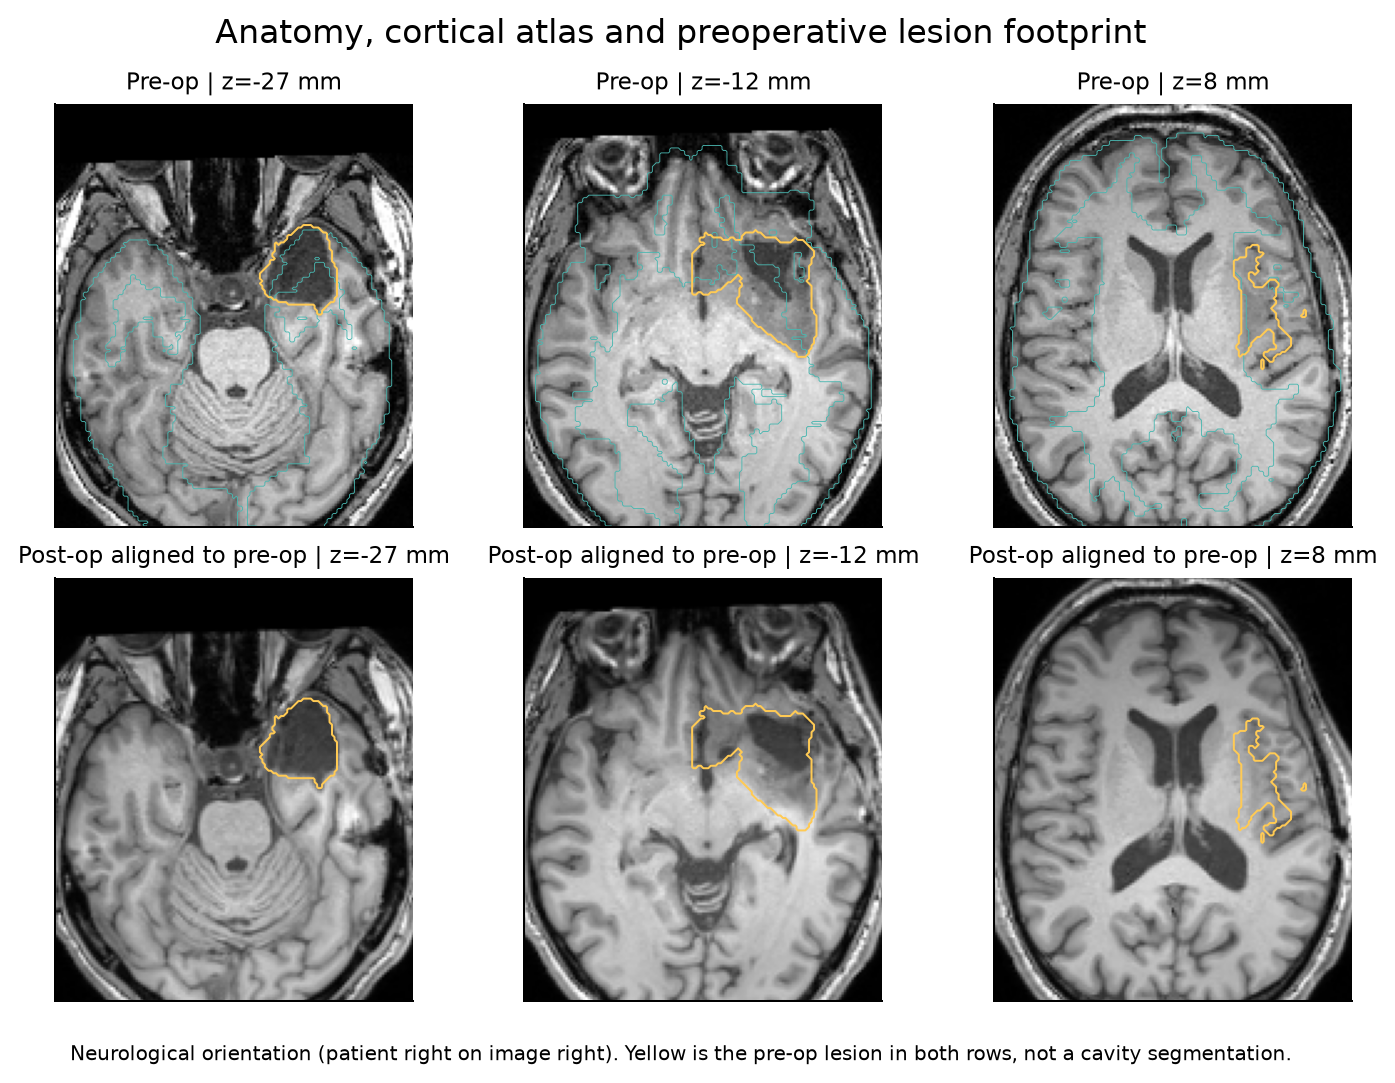
\includegraphics[width=\linewidth]{anatomy.png}
\caption{Preoperative and aligned postoperative anatomy. Yellow contours in both rows show the preoperative lesion; cyan marks projected cortical coverage in the first row. Neurological orientation is used. No cavity is segmented.}\label{fig:anatomy}\end{figure}
\begin{figure}[H]\centering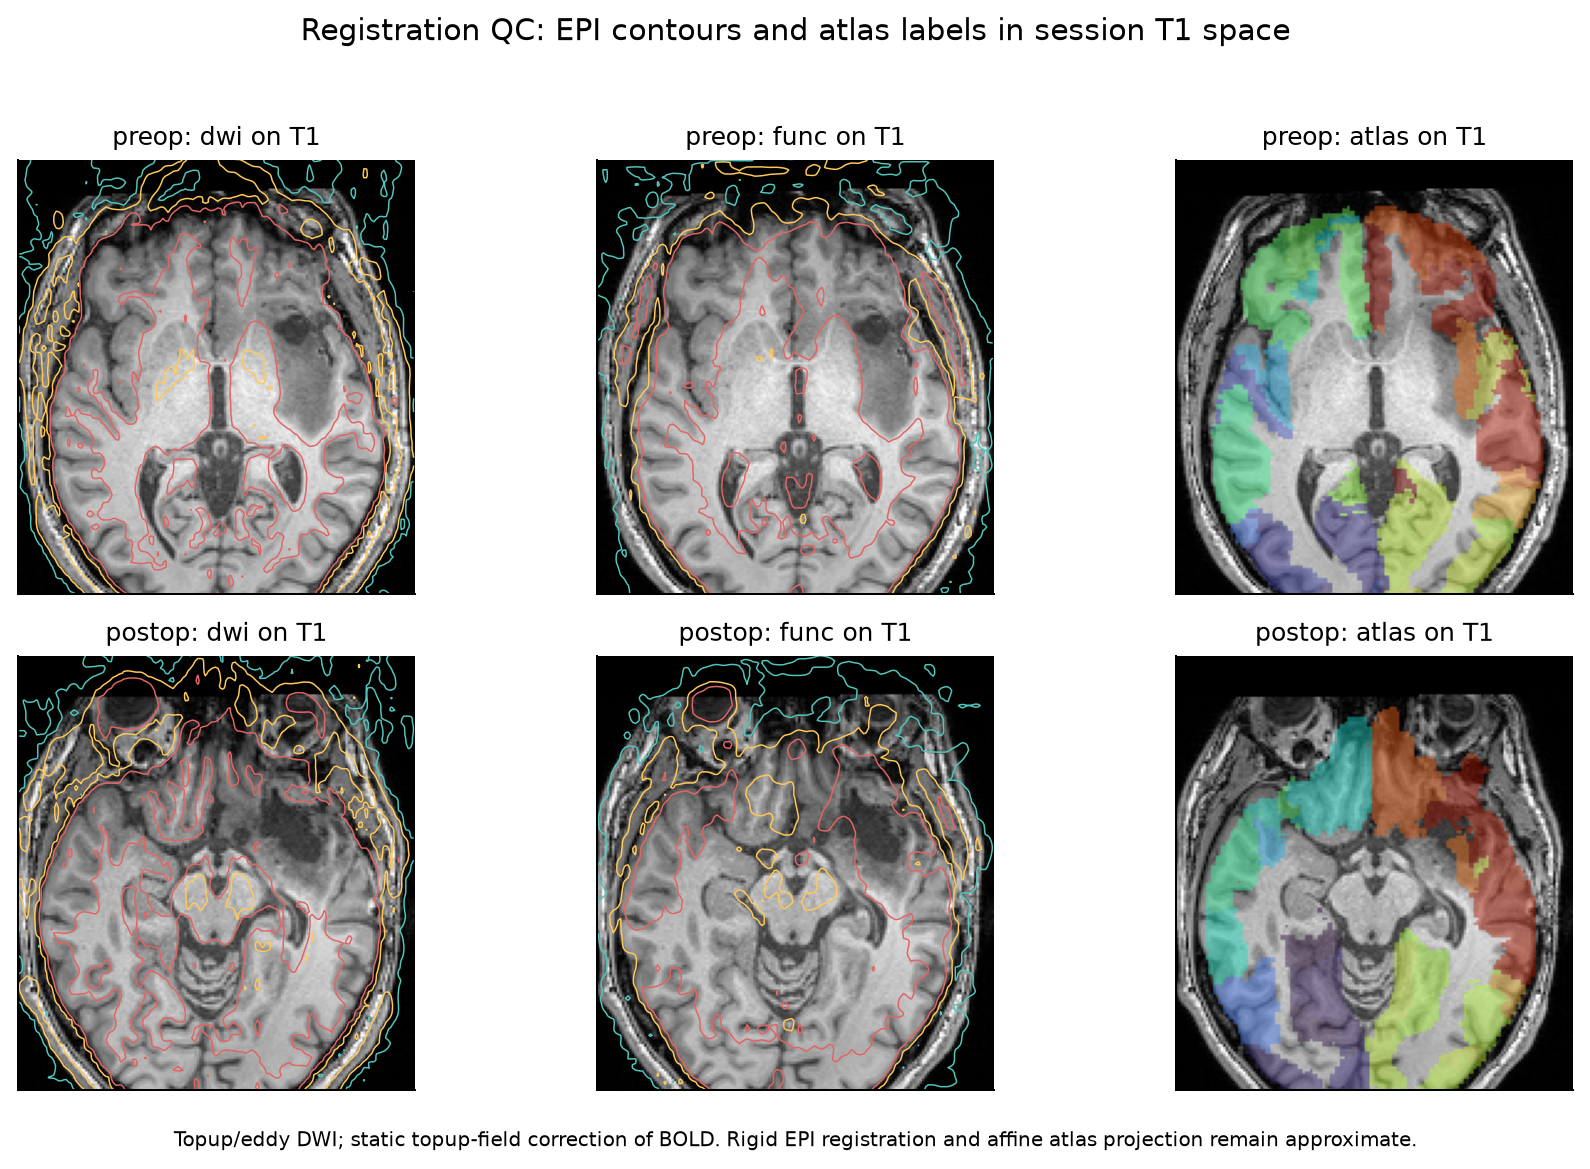
\includegraphics[width=\linewidth]{registration_qc.png}
\caption{EPI intensity contours and atlas labels in session T1 space. These QC slices document approximate alignment, not complete anatomical accuracy; inferior cortex and lesion-adjacent regions remain uncertain.}\label{fig:registration}\end{figure}

\subsection{Structural connectivity}
DIPY \citep{garyfallidis2014} fits weighted-least-squares DTI to b0 and the 700/1200 shells for FA/MD. Single-shell CSD \citep{tournier2007} uses only b0 and $b=2800$ (56 volumes), with spherical-harmonic order 6. The single-tissue response uses median tensor eigenvalues fitted to that same high shell and median b0 signal, in brain voxels selected using low-shell FA$>0.7$ and $0<\mathrm{MD}<0.002$ mm$^2$/s. The original deterministic maximum-direction tracking uses 30,000 random seed locations per session (seed 160); the primary repeat-based policy below uses 20 new runs at the same per-run budget, FA$>0.25$ seeding, FA=0.1 stopping, 0.75-mm steps, a 35-degree turn limit, one initial direction and at most 400 steps per half-streamline. Retained lengths are 20--250 mm.

Each endpoint is assigned to the nearest labelled cortical voxel within 6 mm. Both endpoints must pass and belong to different parcels. The original symmetric count $C_{ij}$ gives historical sensitivity weights
\begin{equation}W_{ij}=C_{ij}/\sum_{i<j} C_{ij}.\end{equation}
Original counts per 10,000 seeds and radii 2, 4 and 8 mm are also saved. Primary support and weights now use the repeat-based policy in Section~\ref{sec:primaryscmethods}. A zero means no assigned streamline under this pipeline, not proven absence of a pathway. No ACT or SIFT2 is performed. Fractions are compositional, not axon counts, and tractography has fundamental inverse-problem ambiguities \citep{maierhein2017}.

\subsection{Functional connectivity and QC guards}
ROI means use cortical voxels inside the valid correction mask, with tSNR$>5$ and adequate signal, excluding the transported preoperative lesion footprint in both sessions. At least eight usable voxels are required per ROI. All \CommonNodes{} parcels pass in both sessions; comparisons use this common set. Passing a coverage criterion does not establish physiological validity near tumour.

Four initial frames are discarded. Approximate FD sums absolute translation increments and absolute Euler-angle increments times a 50-mm radius. Frames with FD$>0.5$ mm and the following frame are censored. This Euler-based approximation is not identical to every published FD implementation. Motion can systematically bias FC \citep{power2012}.

Primary joint nuisance regression includes six motion parameters, derivatives and squares of both (24 terms), five PCs from combined anatomical WM/CSF cores, intercept, linear trend and DCT terms below 0.01 Hz. Temporal projection, voxel scaling and PCA are trained only on retained original time indices; all frames are projected with fitted weights. This custom CompCor-inspired recipe is described below. Final regression uses the same retained indices without concatenating censor gaps. Primary FC is Pearson correlation of retained residuals, with high-pass only and no explicit GSR.

At least 60 frames and 15 residual regression degrees of freedom are required. High-pass-only FC was adopted after an earlier band-pass analysis failed this guard. Sensitivities use FD thresholds 0.3 and 1.0 mm, whole-brain GSR and 0.01--0.1-Hz band-pass where eligible. Each FD threshold refits anatomical PCA on its own retained samples. GSR uses the mean valid brain signal outside the lesion footprint, including in the notebook control.

\subsection{Primary denoising recommendation and justification}
We recommend retained-frame anatomical five-PC regression (\texttt{anatomical5}) for both PAT16 sessions. This is a \emph{post hoc methodological recommendation} made after the documented sensitivity investigation, not a preregistered choice or a demonstrated patient-specific optimum. The decision prioritizes anatomical nuisance compartments, exclusion of censored samples from PCA training and a fixed model budget. It is not optimized for low mean FC, high SC--FC coupling or agreement with cognition. The frozen specification is recorded in \texttt{config/PRIMARY\_DENOISING.md}.

CompCor motivates representing nuisance variation with multiple tissue-derived directions \citep{behzadi2007}; aCompCor studies support its use relative to tissue means in other populations \citep{muschelli2014}. Cohort benchmarking shows tradeoffs among motion removal, distance dependence, network structure and temporal degrees of freedom, without a universally optimal strategy \citep{ciric2017}. These studies motivate the approach, not its efficacy in PAT16. Our combined five-PC recipe is not the separate WM5+CSF5/12-motion recipe benchmarked by Ciric et al.; we retain separate-tissue regression as a sensitivity.

The anatomical masks target WM/CSF more directly than historical noncortical masks, whose FAST-derived mean GM fraction is about 0.19. Retained-frame training avoids estimating tissue PCs from discarded motion spikes. Five combined PCs preserve the preceding component budget and \PreDof{}/\PostDof{} residual df, while allowing more nuisance directions than two tissue means. Five is a pragmatic fixed count, not an empirically validated optimum; combined PCA weights more WM than CSF voxels. Ten separate-tissue PCs remain eligible and useful, but add complexity without independent evidence of better neural specificity. Selecting a variance-fraction rule would permit unequal session model sizes and is not adopted here.

FD 0.5 mm retains \PreMinutes{}/\PostMinutes{} minutes; FD 0.3 mm leaves only 29/57 residual df and is a refitted sensitivity. No explicit GSR is used in the primary estimand, but substantial global/shared neural variance can still be removed by anatomical regression. Band-pass filtering is retained only where the df guard passes. Modest PVE-threshold dependence and the smaller BOLD processing gap support practical usability, not physiological validation. PC-count dependence, unvalidated tissue labels and absent physiological recordings remain material limitations; one case cannot supply a cohort QC--FC benchmark.

\subsection{Nuisance-PC investigation and anatomical denoising}
Historical primary FC, tables and report are archived under \path{results/before_primary_anatomical5}. The anatomical primary model replaces it in all main residuals, FC, graphs, network resampling and coupling; SC and spatial preprocessing are unchanged. Diagnostic regressions hold corrected cortical ROI signals, saved motion, censoring, SC and 100 common nodes fixed while varying only the nuisance regressors. We reconstruct historical noncortical PCA and compare subspaces, rather than arbitrary PC signs. Sweeps retain 0--20 PCs. Partial cortical-mean $R^2$ is the in-sample fraction of variance removed from the unweighted mean of the cortical ROI residuals beyond identical base motion/trend/DCT regression; it is not noise-specific explained variance or an out-of-sample fit.

A factorial diagnostic crosses three PCA images (historical linear motion resampling, matched cubic motion resampling with zero field, and cubic static-field correction) with four masks (historical, refitted, historical restricted to corrected field support, and their intersection). The cubic zero-field control uses identical raw data, saved motion, sampler and reference grid, with zero PE displacement and unit Jacobian. A linear-coordinate audit against saved SimpleITK resampling uses five distributed frames per session and interior nuisance voxels. Corrected ROI signals stay fixed even when the diagnostic PCA image changes. Mixed image/mask pairs isolate computational dependencies on this numeric grid; they do not preserve physical tissue correspondence after unwarping or define preferred complete pipelines.

For the anatomical primary and sensitivity models, FSL FAST performs bias-corrected, T1-only three-class partial-volume segmentation \citep{zhang2001,fastdocs}. Its input uses the existing session brain mask, positive T1 intensities and exclusion of the lesion footprint plus 5 mm; the postoperative footprint is not a cavity segmentation. FAST's CSF/GM/WM fractions are tissue-model estimates, not manually validated probabilities of correct classification. WM and CSF native masks require fraction $\geq0.95$, $>2$ mm brain interior and 1-mm erosion before BOLD resampling. Nearest-neighbour core membership and linearly interpolated tissue fraction $\geq0.95$ must both pass, together with BOLD support and lesion exclusion. CSF includes ventricular and sulcal regions. No independent tissue labels are available.

Six complete denoising models use each BOLD package's fixed cortical signals and identical motion/DCT/censoring: base regression only; historical noncortical five PCs; anatomical five PCs with the historical all-180-frame PCA recipe; anatomical five PCs trained on retained frames; separate WM5+CSF5 (ten PCs total); and two WM/CSF means. For retained-frame PCA, constant/linear/low-frequency DCT terms are projected out, voxel scaling and PCA are fitted on retained original time indices, and all frames are projected with the fitted spatial weights. Final joint regression retains the original temporal basis. This custom anatomical component regression is inspired by CompCor \citep{behzadi2007}, without claiming equivalence to another software pipeline. No explicit GSR is added. Sensitivities vary fraction threshold (0.90/0.95/0.99), component count (2/5/10), and FD threshold (0.3 mm, with PCA refitted on its retained samples). Anatomical retained-frame five-PC regression is primary; the other five models and parameter variants remain sensitivity analyses. None is selected to match cognition.

\subsection{Censoring decomposition and matched frame selection}\label{sec:censoringmethod}
A post hoc investigation separates three changes confounded by stricter censoring: the correlation samples, final regression coefficients and the tissue-PC training set. Starting with primary residuals and primary frames, we restrict the same residuals to strict frames, refit final regression on those frames with primary PCs fixed, then refit tissue temporal projection/scaling/PCA and final regression. These ordered increments diagnose computational dependencies, not causal variance fractions. Primary images, masks, motion, SC and FC derivatives remain unchanged.

For both primary and strict eligible pools, 200 draws retain 68 frames per session (2.72 minutes of exposure): (i) independent uniform duration-only sampling without replacement, (ii) duration plus FD matching and (iii) duration plus FD and acquisition-half matching. Both motion protocols use an absolute 0.015-mm paired-FD caliper. Random-cost maximum-cardinality bipartite assignment uses independent uniform costs on eligible pairs and penalty 10,000 otherwise; 68 valid pairs are sampled without replacement. The third protocol additionally requires paired frames to occupy the same original 90-frame run half. Selection uses motion, original indices and seeds, never FC, SC or cognition. This targets common motion support rather than uniform samples of the original pools; paired frames do not represent corresponding neural states.

Feasibility determines this explicit tolerance: strict pools permit 68 FD-only pairs at 0.010 mm, but only 65 with half matching and 56 with third matching. At 0.015 mm the halves permit 68 and thirds only 60. We use the same 0.015-mm tolerance in both motion protocols. Half matching controls coarse time occupancy, not exact times, finer temporal distribution or vigilance. The strict preoperative pool contains exactly 68 frames and remains fixed across its draws. Seeds are 3160 plus protocol index; every selected mask is saved.

Each draw is evaluated with primary PCs/regression coefficients frozen and with complete retained-frame tissue preprocessing/PCA and regression refitting. The original 180-frame temporal basis and gaps remain intact. Complete refits have rank 39 and 29 algebraic residual df; frozen fits are sampling diagnostics trained on more observations, without an inferred subset effective df. Retained exposure is neither contiguous scan duration nor independent sample count. Acquisition span and sample count both influence FC reliability \citep{birn2013}. We save retained FD, standardized mean difference (SMD), KS and Wasserstein distances, paired gaps, time occupancy, span and fragmentation. Matching FD does not match all motion artifacts or physiology.

Median, empirical 2.5/97.5 percentiles and positive-draw fraction describe conditional sampling-design spread, not confidence intervals, surgical-effect probabilities, p values or test--retest reliability. Single-frame sampling does not model serial dependence. Secondary coupling controls restrict SC support to the intersection of nonzero edges, first retaining session weights and then fixing preoperative weights; these explicitly change the estimand. Full design details and source/code hashes are in \path{config/CENSORING_MATCHING.md} and \path{results/censoring_investigation}.

\subsection{Edge-support and network accounting of coupling sensitivity}\label{sec:edgemethod}
We localize the sensitivity of the longitudinal statistic, defining $\Delta_a=\rho_{post,a}-\rho_{pre,a}$ and $R=\Delta_{strict}-\Delta_{primary}$. For each session/fit, let $x_e,y_e$ be centered average ranks of positive SC counts and the corresponding FC values over that session's complete nonzero-SC support. Average ranks handle ties \citep{scipyranks}; counts and $\log(1+\mathrm{SC\ fraction})$ have identical ordering. Define
\begin{align}
 c_e&=\frac{x_e y_e}{\sqrt{\sum_k x_k^2\sum_k y_k^2}},\qquad \rho=\sum_e c_e,\\
 r_e&=(c_{post,strict,e}-c_{pre,strict,e})-(c_{post,primary,e}-c_{pre,primary,e}).
\end{align}
On the union of nonzero SC supports, an absent edge has zero \emph{accounting contribution}; its measured FC is not zero-imputed or included in that session's ranks. Summing $r_e$ by shared/pre-op-only/post-op-only support or by unordered atlas network pair exactly recovers $R$. Global ranks and denominators remain those of the original full supports. These terms are not subgroup-only Spearman coefficients or independent edge effects. Within-/between-group covariance terms, using the same global ranks and denominator, are exported to distinguish covariance within a group from its mean rank location.

We separately recompute all ranks and normalizers after deleting each support group, each of 28 network pairs, all edges incident on each of seven networks, and each individual union edge. Cumulative deletion of 1/5/10/25/50/100 highest positive, negative or absolute $r_e$ edges is a post hoc stress test. Network-incident sets overlap; deletion effects are not additive. All 6$\times$200 previous matched masks are replayed under frozen/refitted nuisance fits. Edge contributions must reproduce every previous matched contrast. A same-frame refitting contrast subtracts frozen from refitted $\Delta$; it is distinct from the original full-sample $R$. Group means sum for disjoint partitions, but marginal medians/quantiles generally do not.

Source node IDs/atlas labels, SC counts, measured FC, FC ranks and edge terms are retained. Centroid distances and endpoint proximity to the preoperative footprint do not establish tract traversal or cavity damage. Session-specific SC presence denotes reconstruction, not demonstrated tract loss/gain. No edgewise p values, independent-edge confidence intervals, treatment effects or cognitive localization are inferred. The full specification is in \path{config/COUPLING_EDGE_DRIVERS.md}.

\subsection{Conditional SC reliability: repeated tracking and count cutoffs}\label{sec:screliabilitymethods}
For each session we generate 20 new tractograms at the original 30,000-seed budget, using RNG initializations 17000--17019 pre-op and 18000--18019 post-op. The DIPY random-seed-location generator \citep{dipytracking} varies seed positions/order while the CSD model, FA/brain masks, geometry, deterministic direction getter, stopping/length rules and 6-mm endpoint assignment remain fixed (Section~3.4). These are new trajectories, not resampled existing streamlines. The original direction getter used float64 CSD coefficients, whereas its saved cache was float32. We refit the identical high-shell CSD model/response once to recover float64 coefficients and require a separate seed-160 replay to reproduce each original SC count matrix exactly. Original inputs/outputs are fingerprinted and retained. Seed coordinates, endpoint pairs/distances/lengths, counts and QC are saved per run.

For all 4,950 cortical pairs, detection at inclusive cutoff $k\in\{1,2,3,5,10,20\}$ means at least $k$ assigned streamlines in one 30,000-seed run. Occurrence is detections/20; count SD/CV include zero-count runs; all-zero means have undefined CV and are excluded from median CV. Original shared/pre-only/post-only/absent labels stay fixed so opposite-session rediscovery can be measured. Pairwise within-session support Jaccard and count-rank agreement over all 4,950 edges are exported. A fixed first/last-ten split selects 80\% consensus in one half and measures occurrence in the other, with roles reversed. This tests consistency under seeding, not independent anatomy.

SC--FC coupling is recomputed at every cutoff for the original matrices and all $20\times20$ pre/post repeat combinations, using unchanged primary/strict FC. Own support applies cutoffs separately; common support uses the intersection with each session's own count weights. All ranks/normalizers are recalculated; SC-absent FC values are excluded. The 400 combinations reuse runs and are dependent. Empirical percentiles and reversal fractions describe conditional seeding variability, not confidence intervals, treatment probabilities or 400 independent replications.

Consensus controls require detection fractions $p\in\{.5,.8,.95,1\}$ at each $k$, weighted by mean counts per 30,000 seeds. Cutoffs apply within each run, not to the 600,000-seed pooled count. Own/common consensus supports are separately evaluated. An 80\% pre-only consensus label permits sub-80\% post-op detection; a separate flag marks 80\% occurrence in one session and zero hits in the other. Neither establishes biological absence. Original reversal terms are cross-tabulated by repeat consensus class; re-ranked terms are also exported by original support, repeat class and network pair for every fixed reference.

All six preceding 200-draw matching protocols are replayed with full nuisance refitting while holding five SC references fixed: original own SC at $k=1,3,5$, and 80\% consensus at $k=1$ with own/common support. The $k=1$ controls must reproduce all preceding matched results. These historical controls vary FC sampling at fixed SC, complementing repeated SC at fixed FC. Joint FC--seed variability under the recommended policy is now quantified separately in Section~\ref{sec:jointresults}. Thresholds/occurrence fractions are reported as sensitivity settings and are never selected by coupling sign. Systematic false pathways can be reproducible \citep{maierhein2017}; fixed-image seeding does not test acquisition noise, model/registration error, endpoint validity or scan--rescan reliability. Details are in \path{config/SC_RELIABILITY.md}.

\subsection{Recommended primary SC support and weighting}\label{sec:primaryscmethods}
We make a post hoc methodological recommendation based on conditional seed stability and comparable edge populations, without optimizing a coupling sign or agreement with CANTAB. Prior FC results were available: this decision was not blinded or preregistered. For session $s$, repeat $r$ and edge $e$, define
\begin{equation}
\begin{aligned}
 H_{s,e}&=\sum_{r=1}^{20}\mathbf{1}(C_{s,r,e}\geq1),&
 S_s&=\{e:H_{s,e}\geq16\},\\
 \bar C_{s,e}&=\frac{1}{20}\sum_{r=1}^{20}C_{s,r,e},&
 W_{s,e}&=\mathbf{1}(e\in S_s)\frac{10{,}000}{30{,}000}\bar C_{s,e}.
\end{aligned}
\end{equation}
Zeros enter the mean; we neither average only successful detections nor multiply by occurrence again. Eighty percent permits four misses while rejecting intermittent edges. It is a pragmatic boundary, not a calibrated anatomical threshold or a demonstrated optimum. Singleton median occurrence (55\%/50\%), high-count median occurrence (100\%/100\%) and the split-half diagnostics motivate repeated support rather than one arbitrary run or an aggressive count cutoff that also removes stable weak reconstructions. The same runs select support and estimate weights; split halves diagnose consistency, not independent validation of final weights.

SC matrices, graphs, network means and preoperative simulations use each session's own consensus $S_s$. Primary longitudinal coupling instead uses $S_{pre}\cap S_{post}$, further restricted to finite FC nodes in both sessions, with each session's own $\bar C$ weights. This compares ranks of SC and FC on the same reconstructed connections. Own-support coupling remains a prominent complementary sensitivity: it includes changing topology but also changes the ranked edge population. Common support excludes 337/340 session-specific consensus connections and conditions on both scans; it cannot measure disconnection or serve as a prospective preoperative predictor. Applying that intersection to all structural graphs would also discard those topology differences, so we keep these two estimands explicit.

The fixed attempted-seed denominator avoids the additional compositional constraint of dividing by each session's total assigned streamlines. Mean counts smooth single-run discretization; positive scalar rescaling preserves Spearman ranks, but session-specific fraction normalization can alter longitudinal weighted graph comparisons. Rates remain sampling yields: seed-mask size, geometry, endpoint assignment and tracking yield can differ. They are not axon counts, fibre density or calibrated biological connectivity; no ACT/SIFT2 is implemented \citep{maierhein2017,mrtrixconnectome}. Stable false paths can recur. Original fractions, unfiltered repeat means, count cutoffs, own/common supports, 50/95/100\% consensus, all repeat pairs and denoising/matching alternatives are retained. The frozen rule is in \path{config/PRIMARY_SC.md}; the preceding main delivery is archived under \path{results/before_primary_sc}.

\subsection{Joint tractography and FC sampling design}\label{sec:jointmethods}
The preceding controls perturb one source at a time. We now cross SC and FC perturbations under the recommended primary strategy, retaining the observed point estimates and all historical sensitivities. Each of 500 SC bootstrap draws samples 20 whole tractography runs with replacement independently within each session, recomputes the all-run mean including zeros, and retains the attempted-seed denominator. This resamples the 20-run estimator, not one noisy tractogram. Edges within each run remain dependent. Pre/post random streams are separate (seeds 4160/4161); the original seed-160 run is excluded and run numbers are not paired across sessions.

The primary conditional-support experiment locks the observed 823-edge intersection and varies its mean weights. A selection sensitivity recomputes the inclusive 16/20 consensus in each session and uses the draw's intersection, reranking both SC and FC on that population. Selection sensitivity changes the population of connections; its distribution is not the identical fixed-support estimand. Bootstrap consensus remains conditional on just 20 empirical runs and on the same diffusion images, model and geometry.

FC has two complementary resampling branches, each with 200 paired pre/post draws. First, full-run primary and strict analyses draw circular blocks of 10 original frames (24 s), discard censored members within each block, and continue until the original retained count is reached, then truncate. All 100 ROI residuals use the same sampled indices. Blocks are drawn on the original 180-frame axis, never a concatenated uncensored series. Five- and twenty-frame blocks (12/48 s) are fixed sensitivities. Circular blocks address temporal dependence \citep{bellec2008}; we do not transfer that paper's hypothesis-test calibration to this censored rank statistic. This branch freezes each session's censor-specific fitted residuals: it measures temporal sampling conditional on nuisance training. Repeated indices reduce distinct-frame counts, saved in QC; the original residual df is not assigned to bootstrap draws. Circular stationarity, including across run endpoints, is approximate.

Second, we exactly reuse all six saved 200-mask duration/FD/run-half protocols, retaining 68 distinct frames per session. Tissue temporal projection, scaling, five-PC extraction and nuisance regression are fully refitted on every mask, retaining the original temporal basis. These draws are subsamples without replacement, not a temporal bootstrap. Strict pre-op has exactly 68 eligible frames: every strict matched draw has identical pre-op FC, so its FC variability comes from post-op selection alone. Duration and measured FD matching do not equate physiological noise, neural states, serial dependence or independent information.

Every SC draw is crossed with every paired FC draw, yielding 100,000 dependent cells per protocol and support mode. Let $D_{bf}=\rho_{post,bf}-\rho_{pre,bf}$. Average tied ranks and normalizers are recomputed for each selected support. We report joint medians, 2.5/97.5 percentiles, SD and empirical positive fractions. SC-only anchors retain observed full-run FC; FC-only anchors retain the observed SC weights/support. Their percentiles cannot be added. In a matched design the SC-only anchor is not the SC main effect averaged over FC subsets. For the crossed grid,
\begin{equation}
\begin{aligned}
 a_b&=\overline D_{b\cdot}-\overline D,&
 c_f&=\overline D_{\cdot f}-\overline D,\\
 u_{bf}&=D_{bf}-\overline D-a_b-c_f,&
 \operatorname{Var}_{bf}(D)&=\operatorname{Var}_b(a)+\operatorname{Var}_f(c)+\operatorname{Var}_{bf}(u).
\end{aligned}
\end{equation}
Population variances (ddof=0) give this exact finite-grid identity under independent product resampling weights. Shares describe this computational experiment, not identified biological error sources. Reused rows/columns invalidate independent-cell standard errors or binomial uncertainty based on 100,000 cells. Half-ensemble checks assess finite Monte Carlo sensitivity without proving convergence.

These conditional ranges are not calibrated confidence intervals for neural change or probabilities of a surgical effect. Neither branch resamples acquisition/image noise, registration, masks, diffusion-model/endpoint choices, haemodynamics or clinical assessments. This original frozen full-run branch omits nuisance-training uncertainty; the matched branch conditions on short eligible pools and its selection design. \path{config/JOINT_SAMPLING.md} fixes all choices; \path{results/joint_sampling} stores every sampled run index, SC weight/support, FC vector, block index, matched mask, crossed grid and source/output fingerprint. The preceding delivery is preserved in \path{results/before_joint_sampling}.

\subsection{Full-run nuisance refitting and descriptive clinical integration}\label{sec:refitmethods}
The frozen full-run branch above conditions on estimated nuisance training. We extend it using exactly the same 200 saved paired block draws per pool/length and the same 500 whole-run SC bootstrap draws. Three conditions are paired: (i) frozen residuals; (ii) fixed censor-pool PC scores with all regression coefficients and design scaling refitted; (iii) full refitting of tissue temporal projection, voxel centering/scaling, five-PC extraction, nuisance-design scaling and regression. All spatial masks, ROI signals, motion, censor eligibility and primary policies remain fixed. This repeated-row full-run bootstrap is retained as a sensitivity alongside the frozen branch and matched designs; the recommended nonreplacement stability design is specified below.

If $w_t$ is the multiplicity of original frame $t$, both temporal tissue projection and nuisance regression minimize $\sum_t w_t\lVert y_t-X_t\beta\rVert^2$. With $W=\operatorname{diag}(w_t)$, weighted centering/scaling and the eigendecomposition of $W^{1/2}ZZ^TW^{1/2}$ reproduce explicitly repeated-row PCA; FC is weighted correlation of refitted ROI residuals. Derivatives are computed once on the original motion trajectory and the DCT basis retains original 180-frame coordinates. Artificial block joins do not define new temporal derivatives. Numerical tests verify repeated-row equivalence, exact replay of the frozen FC and recovery of observed full-run FC to below $10^{-11}$ absolute difference.

Repeated frames carry bootstrap frequency but add no new measured rows. We explicitly extend the existing feasibility guards conservatively to require at least 60 \emph{distinct} frames and at least 15 distinct rows minus design rank, with agreement between numerical design and least-squares solver ranks. This is a new safeguard for this high-parameter, short-run analysis, not a universal bootstrap requirement. Neither sampled count minus rank nor distinct count minus rank estimates independent BOLD information. Every fit is attempted; failures retain QC and unavailable FC rather than being redrawn. All three models are compared on identical eligible paired draws, with a descriptive minimum of 100/200 pairs for publishing a range, fixed before computing contrasts. If rejection occurs, the resulting conditional population can differ; counts must accompany ranges. Complete specifications and hashes are in \path{config/JOINT_REFIT.md} and \path{results/joint_refit}.

For clinical integration, we compute within-network mean Fisher-$z$ FC on all anatomical parcel pairs in each Yeo network using the same primary ten-frame draws. SC network means use own-consensus all-run seed rates, reselecting own 16/20 support on each of the 500 whole-run bootstraps and retaining zeros over the fixed within-network pair population. These are different summaries from coupling on 823 shared SC edges. Their separate units and uncertainty sources are retained; no joint cognitive scalar is constructed. A 47-field ledger preserves all raw CANTAB/context values, units, missingness and caveats. Candidate task/network links are the pre-existing didactic hypotheses, not individual localization. Context fields are unlocalized. No two-observation correlation, clinical bootstrap, composite, reliable-change threshold or causal adjustment is estimated.

\subsection{Diagnosing PC-training shifts with block subsampling}\label{sec:pcsamplingmethods}
We investigate empirical recentering of conditional distributions, without identifying population bias or revising observed outcomes. The fixed primary denoising/SC rules and all preceding outputs are retained. Before computing contrasts, \path{config/PC_SAMPLING.md} specified four designs at 5/10/20-frame blocks, each with 200 paired draws and frozen, coefficient-only and full nuisance refits. First, we replay the original frequency-weighted bootstrap. Second, a unit-coverage control assigns weight one to exactly that draw's distinct original frames. This isolates multiplicities at identical coverage; it is not independently sampled block subsampling. Third, true block subsampling without replacement uses a uniformly random circular origin on the original 180 positions, partitions into nonoverlapping tiles, permutes tiles once, omits censored members and trims the final tile to match the exact bootstrap distinct-frame count for each session/draw. Fourth, the same sampler retains $\lfloor0.8n_{eligible}\rfloor=116/120$ pre/post frames. Blocks need not remain contiguous after censoring, and the last tile can be partial. Matching distinct counts does not match motion, physiology or independent information.

Every design retains original-time derivatives/DCT and common ROI draws. The existing distinct-frame/rank safeguards and 100-pair reporting minimum apply; no failed draw is redrawn. All FC draws are crossed with the same 500 whole-run SC bootstraps on the fixed 823 edges. Full refits of the three new ten-frame designs additionally reselect consensus support. We retain session-specific draw QC, temporal coverage, frequency Kish count $(\sum w)^2/\sum w^2$, numerical rank/condition and Monte Carlo half-ensembles. Kish count measures weight concentration, not independent BOLD information. Subsample ranges depend on retained fraction and are not calibrated intervals for the original full-run statistic. At 100\% without replacement the FC fit must equal the observed full-run fit, so FC spread vanishes, while SC seed-sampling variability can remain.

On the original ten-frame bootstrap draws, a $2\times2$ intervention varies tissue preprocessing (temporal projection/voxel scaling) and spatial PCA loadings (baseline versus refitted), with regression coefficients refitted in all conditions. A fifth temporal-only control freezes voxel scales and loadings. If tissue signals change from $Z$ to $Z-TA$ for the already included temporal basis $T$, fixed-loading PC scores change by $-TAV$, inside the same GLM background span. Their residual FC should therefore be invariant. Weighted PC-span comparisons first project out the identical motion/trend/DCT background; their minimum/mean squared cosines differ from earlier raw-score comparisons. We save variance captured by five tissue PCs, relative eigenvalue gap $(\lambda_5-\lambda_6)/\lambda_5$, and cortical/network-mean variance removed by PCs relative to the same draw's background-only GLM. The removed/shared signal is not classified as neural or noise. Paired computational increments depend on intervention order and are not causal percentages. All 47 clinical/context fields retain their values and caveats; the new network ranges supplement their descriptive evidence browser.

\subsection{Recommended primary FC resampling}\label{sec:primaryfcmethods}
We recommend nonreplacement block subsampling of the original 180-frame axis, with complete nuisance refitting, as a descriptive stability analysis. In each session a random circular origin partitions the original time axis into nonoverlapping ten-frame (24-s) tiles. One random tile permutation is traversed, censored members omitted and the last tile trimmed to exactly $m=\lfloor (2/3)\min(146,150)\rfloor=97$ distinct eligible frames per session (3.88 minutes retained exposure). Tiles preserve local adjacency but not all long-range dependence; circular wrapping and a trimmed final tile are explicit approximations. Regression retains original motion derivatives and DCT coordinates rather than constructing an artificial contiguous scan. Fixed images, masks, ROI signals, motion and eligibility are conditional inputs. Tissue temporal projection, voxel scaling, five-PC extraction, design scaling and regression are all retrained within each subset.

The rationale is methodological: avoiding repeated rows removes multiplicity-induced concentration of the learned tissue covariance, while refitting accounts for estimator training on the selected data. Freezing full-pool training conditions on information outside the subset. Equal distinct counts remove unequal retained duration from the primary comparison. Two-thirds approximates the earlier bootstrap's 94/96 median distinct coverage while deliberately omitting a substantial fraction and leaving 58 algebraic residual directions after rank-39 regression. This is a post hoc engineering compromise, not a data-driven optimum, independent sample size or validated inferential calibration. The policy and 50\%/two-thirds/80\% common-pool fractions, crossed with 5/10/20-frame blocks, were saved in \path{config/PRIMARY_FC_RESAMPLING.md} before these new contrasts were calculated; clinical signs did not select them. Future studies need an independently specified design and longer repeated scans.

All 200 pre/post subsets are independently sampled per session; the draw index does not pair physiological time points. They are crossed with the same 500 whole-run SC bootstrap draws on the fixed 823-edge support and session-specific seed-rate weights. Network FC uses all within-network anatomical pairs. We report observed full-run point estimates separately from subset medians and raw 2.5/97.5 percentiles. These percentiles describe conditional stability of the 97-frame estimator, not confidence limits for full-run FC, a bias correction or a probability of a biological effect. No subsampling-theory scaling or full-run coverage claim is made. Dependence among overlapping subsets and the crossed grid also precludes treating 100,000 cells as independent experiments. Fraction, block, frozen/coefficient fits, reselected SC support, previous bootstraps, original session-specific 80\% subsets, strict censoring and 68-frame duration/FD/run-half matching remain explicit sensitivities.

\subsection{Graphs, networks and clinical integration}
Positive graphs retain strongest edges at requested densities 0.10--0.30 in 0.05 increments; achieved density is exported and absent edges are not invented. Signed FC remains available. Weighted shortest-path cost is $1/w_{ij}$, with efficiency
\begin{equation}E=\frac{1}{n(n-1)}\sum_{i\ne j}1/d_{ij},\end{equation}
where disconnected pairs contribute zero \citep{rubinov2010}. SC uses one maximum-weight scale shared across sessions for efficiency and weighted triangle clustering; FC uses scale 1. Binary efficiency, strength, components and largest component are also exported. SC and FC efficiency have different units/scales.

Within-network summaries are mean own-consensus SC weight per 10,000 seeds (including zeros for excluded edges) and mean Fisher-transformed FC, excluding self-connections. The original figure uses 200 ten-frame block resamples with frozen fits. The primary updated network uncertainty additionally refits coefficients and WM/CSF PCs within the same draws (Section~\ref{sec:integration}). All ranges describe conditional within-run sampling instability, not surgery-effect uncertainty. Primary SC--FC coupling is descriptive Spearman correlation on the common-consensus upper-triangle edge population with session-specific mean-count weights; no edge-independence p-value is reported.

All assessments are tabulated as postoperative minus preoperative. Selected plots reverse signs for latency, error and moves to indicate nominally favorable direction; SD measures have no assigned favorable direction. Percent changes are not normative effect sizes. No global cognitive/QoL composite is created. We do not correlate two cognitive observations with two network estimates: a nonconstant two-point correlation is mechanically $\pm1$.

Broad candidate links motivate questions: MOT with sensory/motor and attention systems; RTI with attention, decision and motor execution; RVP with attention/control; SOC with executive control; SSP with visuospatial attention and short-term memory. Group atlas labels are hypotheses about this patient, not individually validated network localization.

\section{Results}
\subsection{Reconstruction yield and quality}
The historical seed-160 reconstruction retained \PreStreamlines{} and \PostStreamlines{} length-filtered streamlines, with \PreAssigned{} and \PostAssigned{} interparcel assignments. Primary FC retained \PreMinutes{} and \PostMinutes{} minutes, with \PreDof{} and \PostDof{} residual degrees of freedom (Table~\ref{tab:qc}). Figure~\ref{fig:matrices} shows newly derived matrices, without any simulated postoperative replacement.
\begin{table}[H]\centering\small\begin{tabular}{lrr}
\toprule
Quantity & Pre-op & Post-op \\
\midrule
Seed-160 length-filtered streamlines & 26488 & 26421 \\
Seed-160 assigned interparcel streamlines & 16258 & 15889 \\
Primary retained BOLD frames & 146 & 150 \\
Primary retained minutes & 5.84 & 6 \\
Residual regression degrees of freedom & 107 & 111 \\
Mean approximate FD (mm) & 0.328 & 0.287 \\
Own-consensus SC edges & 1160 & 1163 \\
Common-consensus coupling edges & 823 & 823 \\
SC--FC Spearman, common consensus & 0.188 & 0.146 \\
\bottomrule
\end{tabular}

\caption{Historical seed-160 reconstruction yield, primary consensus support and FC QC. FD is the saved Euler-based approximation; SC--FC correlations are descriptive.}\label{tab:qc}\end{table}

Diffusion susceptibility, eddy currents and volume motion are corrected. BOLD uses static field transfer; slice timing remains uncorrected. Table~\ref{tab:dwiqc} and Figures~\ref{fig:dwiqc}--\ref{fig:dwimotion} document correction QC. AP/PA b0 agreement is an internal fit check rather than independent anatomical validation. Approximate atlas projection, rigid longitudinal alignment and nonvalidated nuisance-tissue selection remain material limitations. These are provisional research connectomes.
\begin{table}[H]\centering\small\begin{tabular}{lrr}
\toprule
Quantity & Pre-op & Post-op \\
\midrule
AP/PA b0 correlation before & 0.736 & 0.78 \\
AP/PA b0 correlation after & 0.988 & 0.988 \\
Mean absolute movement RMS (mm) & 1.075 & 0.609 \\
Maximum absolute movement RMS (mm) & 1.653 & 0.862 \\
Flagged/replaced slice entries & 6 & 0 \\
AP nonpositive-Jacobian brain voxels & 2 & 3 \\
PA nonpositive-Jacobian brain voxels & 0 & 0 \\
\bottomrule
\end{tabular}

\caption{Diffusion correction QC. Correlations compare AP/PA mean b0 intensities within the corrected brain mask. Motion RMS is eddy's absolute displacement relative to its reference, not BOLD FD. Flagged slice entries are replaced using eddy's model.}\label{tab:dwiqc}\end{table}
\begin{figure}[H]\centering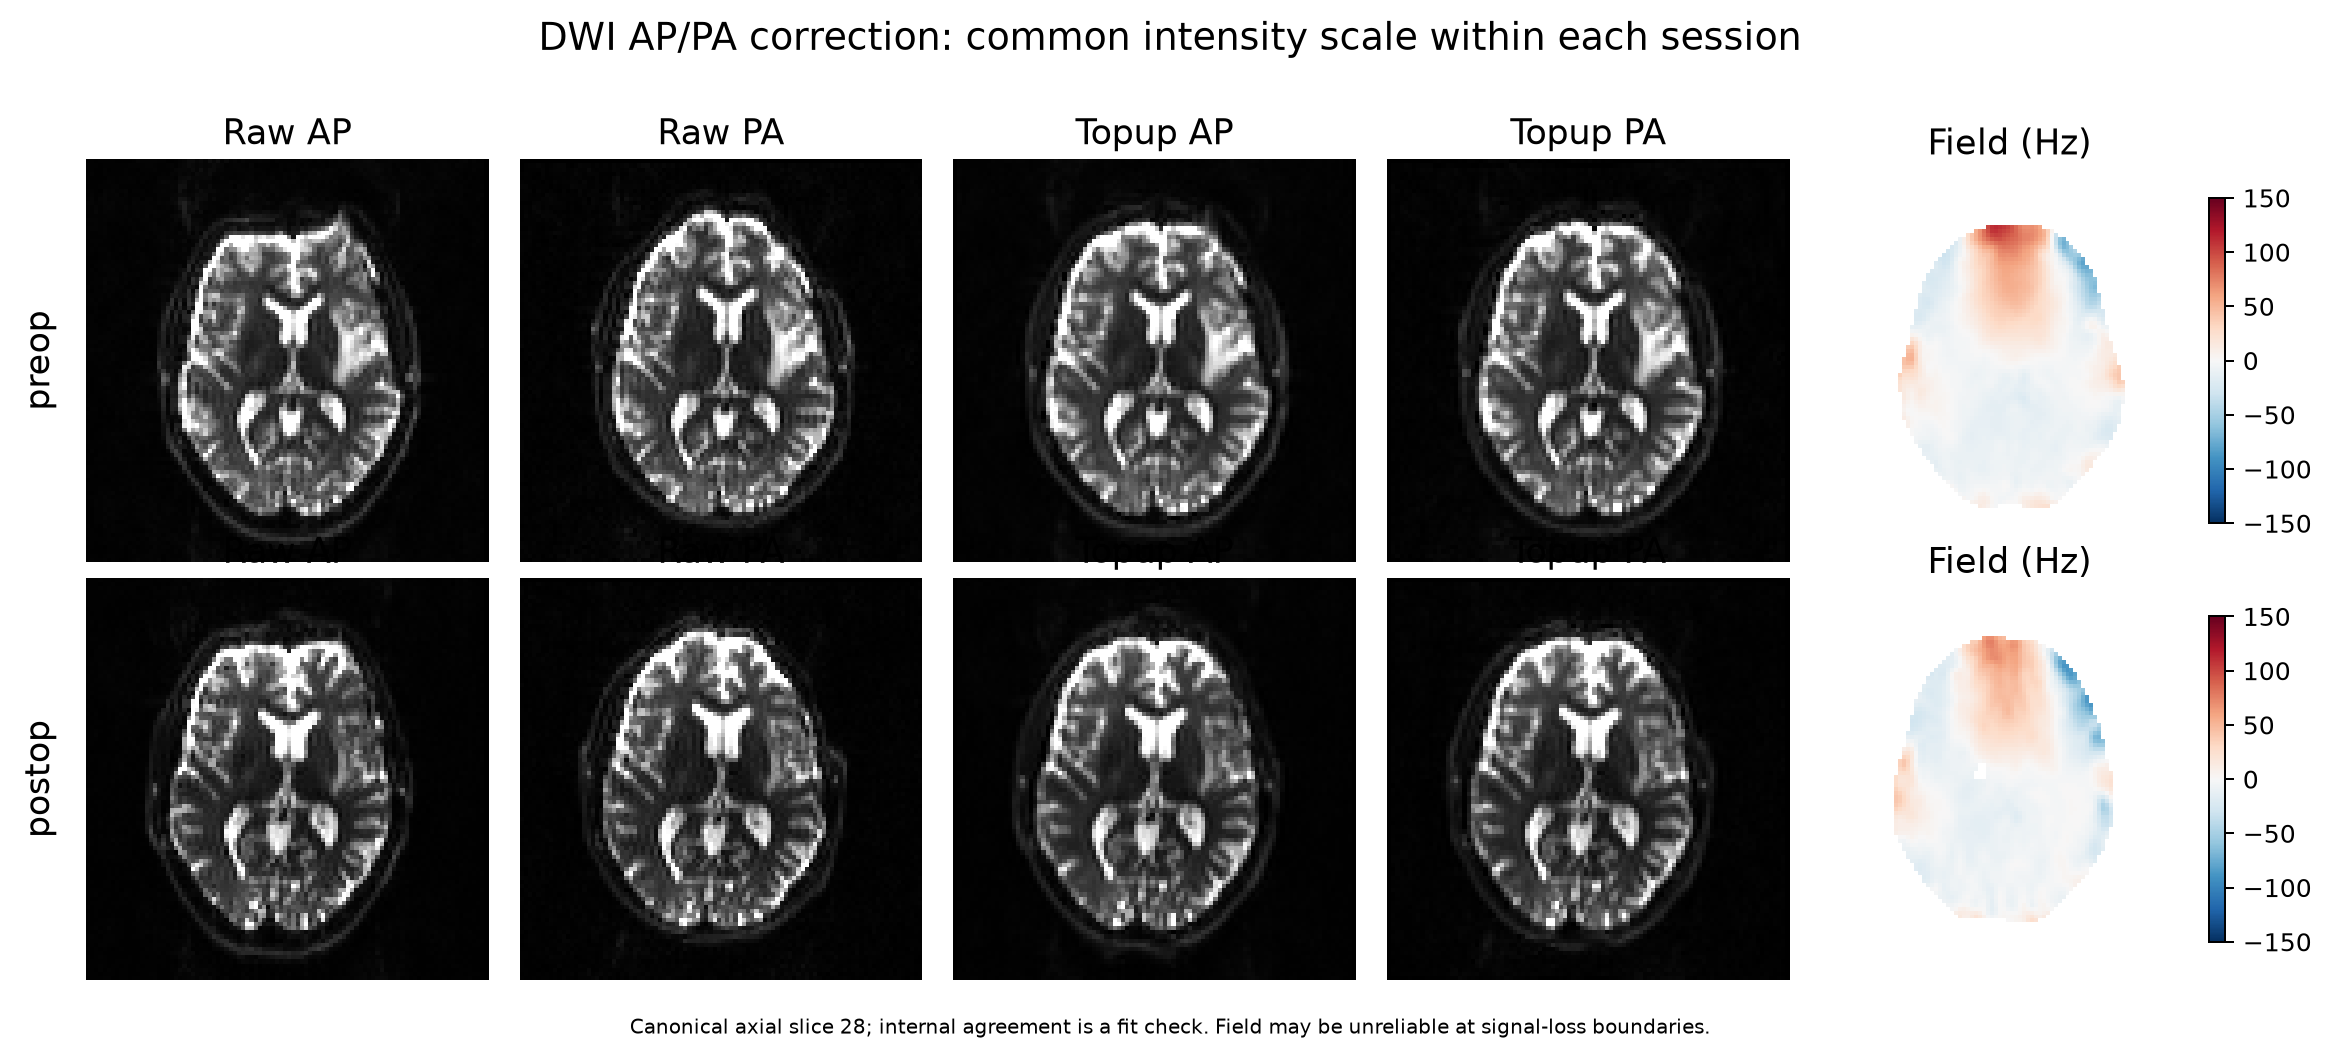
\includegraphics[width=\linewidth]{dwi_distortion_qc.png}
\caption{Raw and topup-corrected AP/PA mean b0s and fitted field. Each session uses a shared intensity scale. Hz scaling is conditional on the supplied readout metadata. Canonical axial slice 28 illustrates agreement; full-volume inspection is available in notebook 01.}\label{fig:dwiqc}\end{figure}
\begin{figure}[H]\centering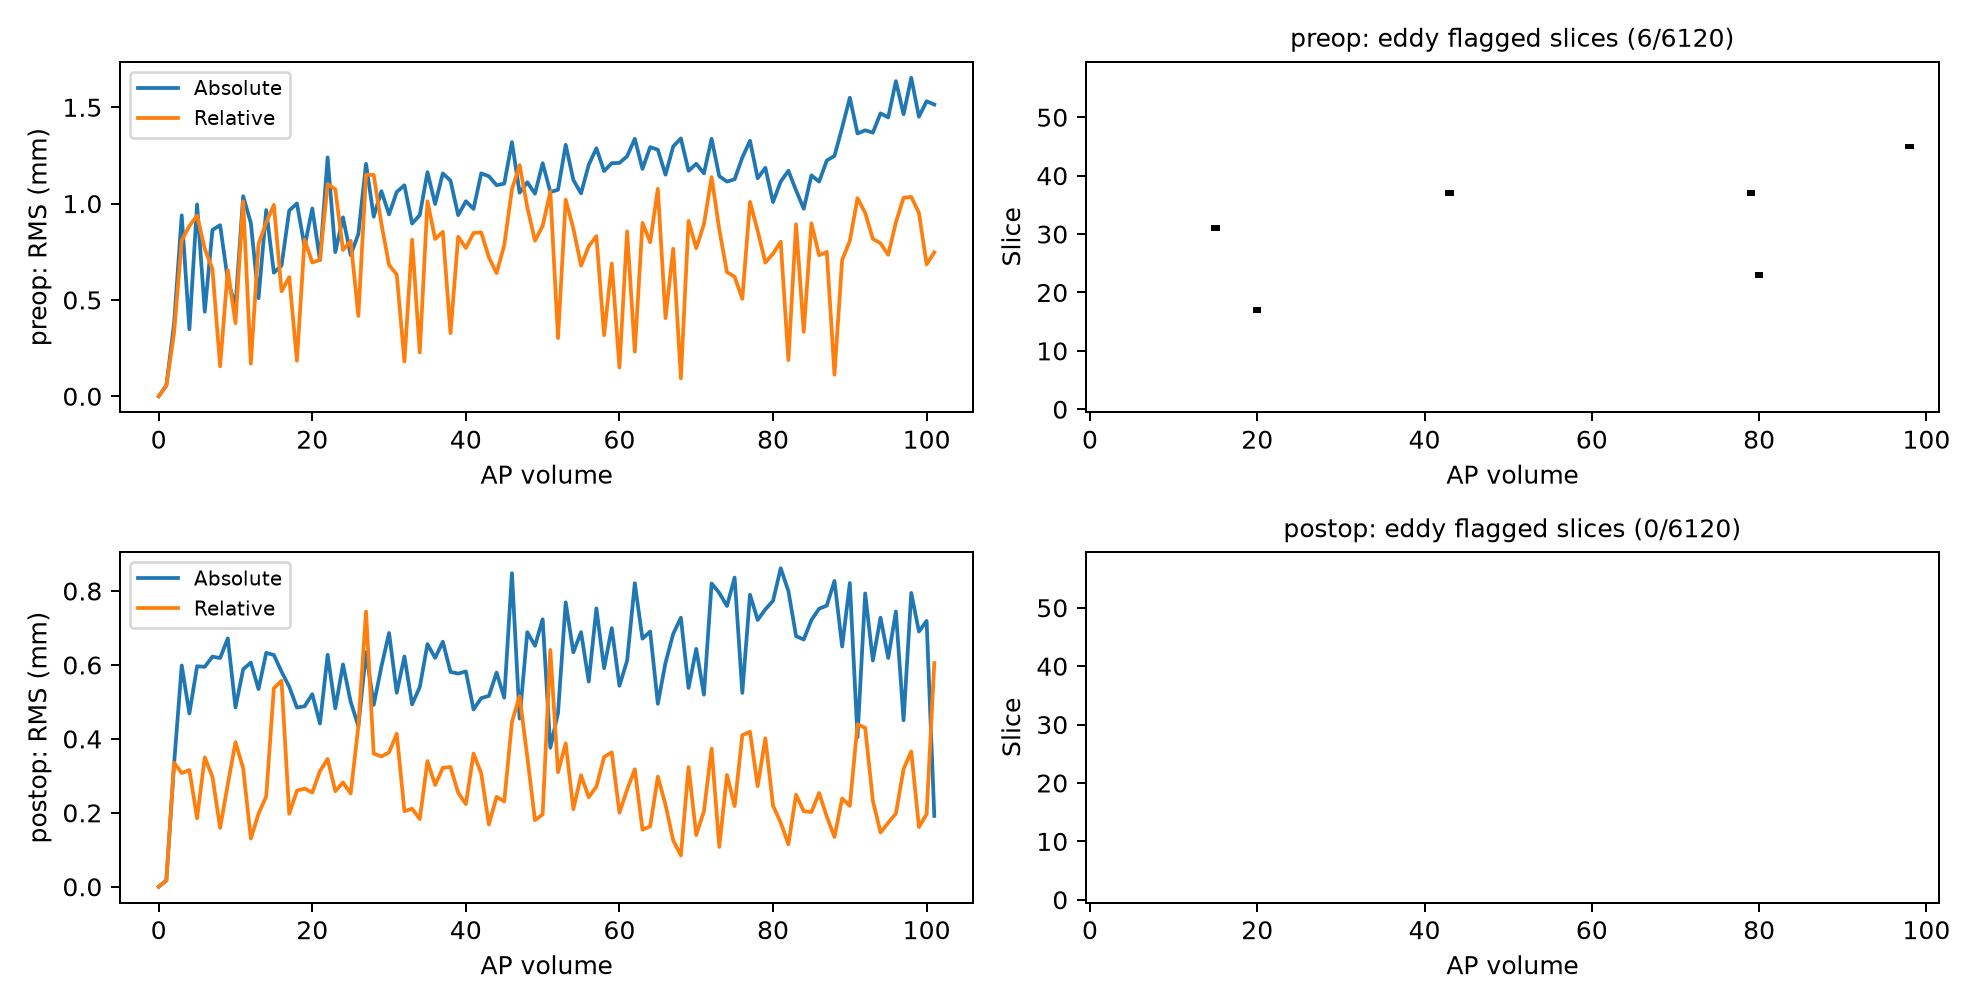
\includegraphics[width=\linewidth]{dwi_motion_outliers.png}
\caption{Eddy absolute/relative movement RMS and flagged slice entries. These complement anatomical and field-map inspection.}\label{fig:dwimotion}\end{figure}
\begin{figure}[H]\centering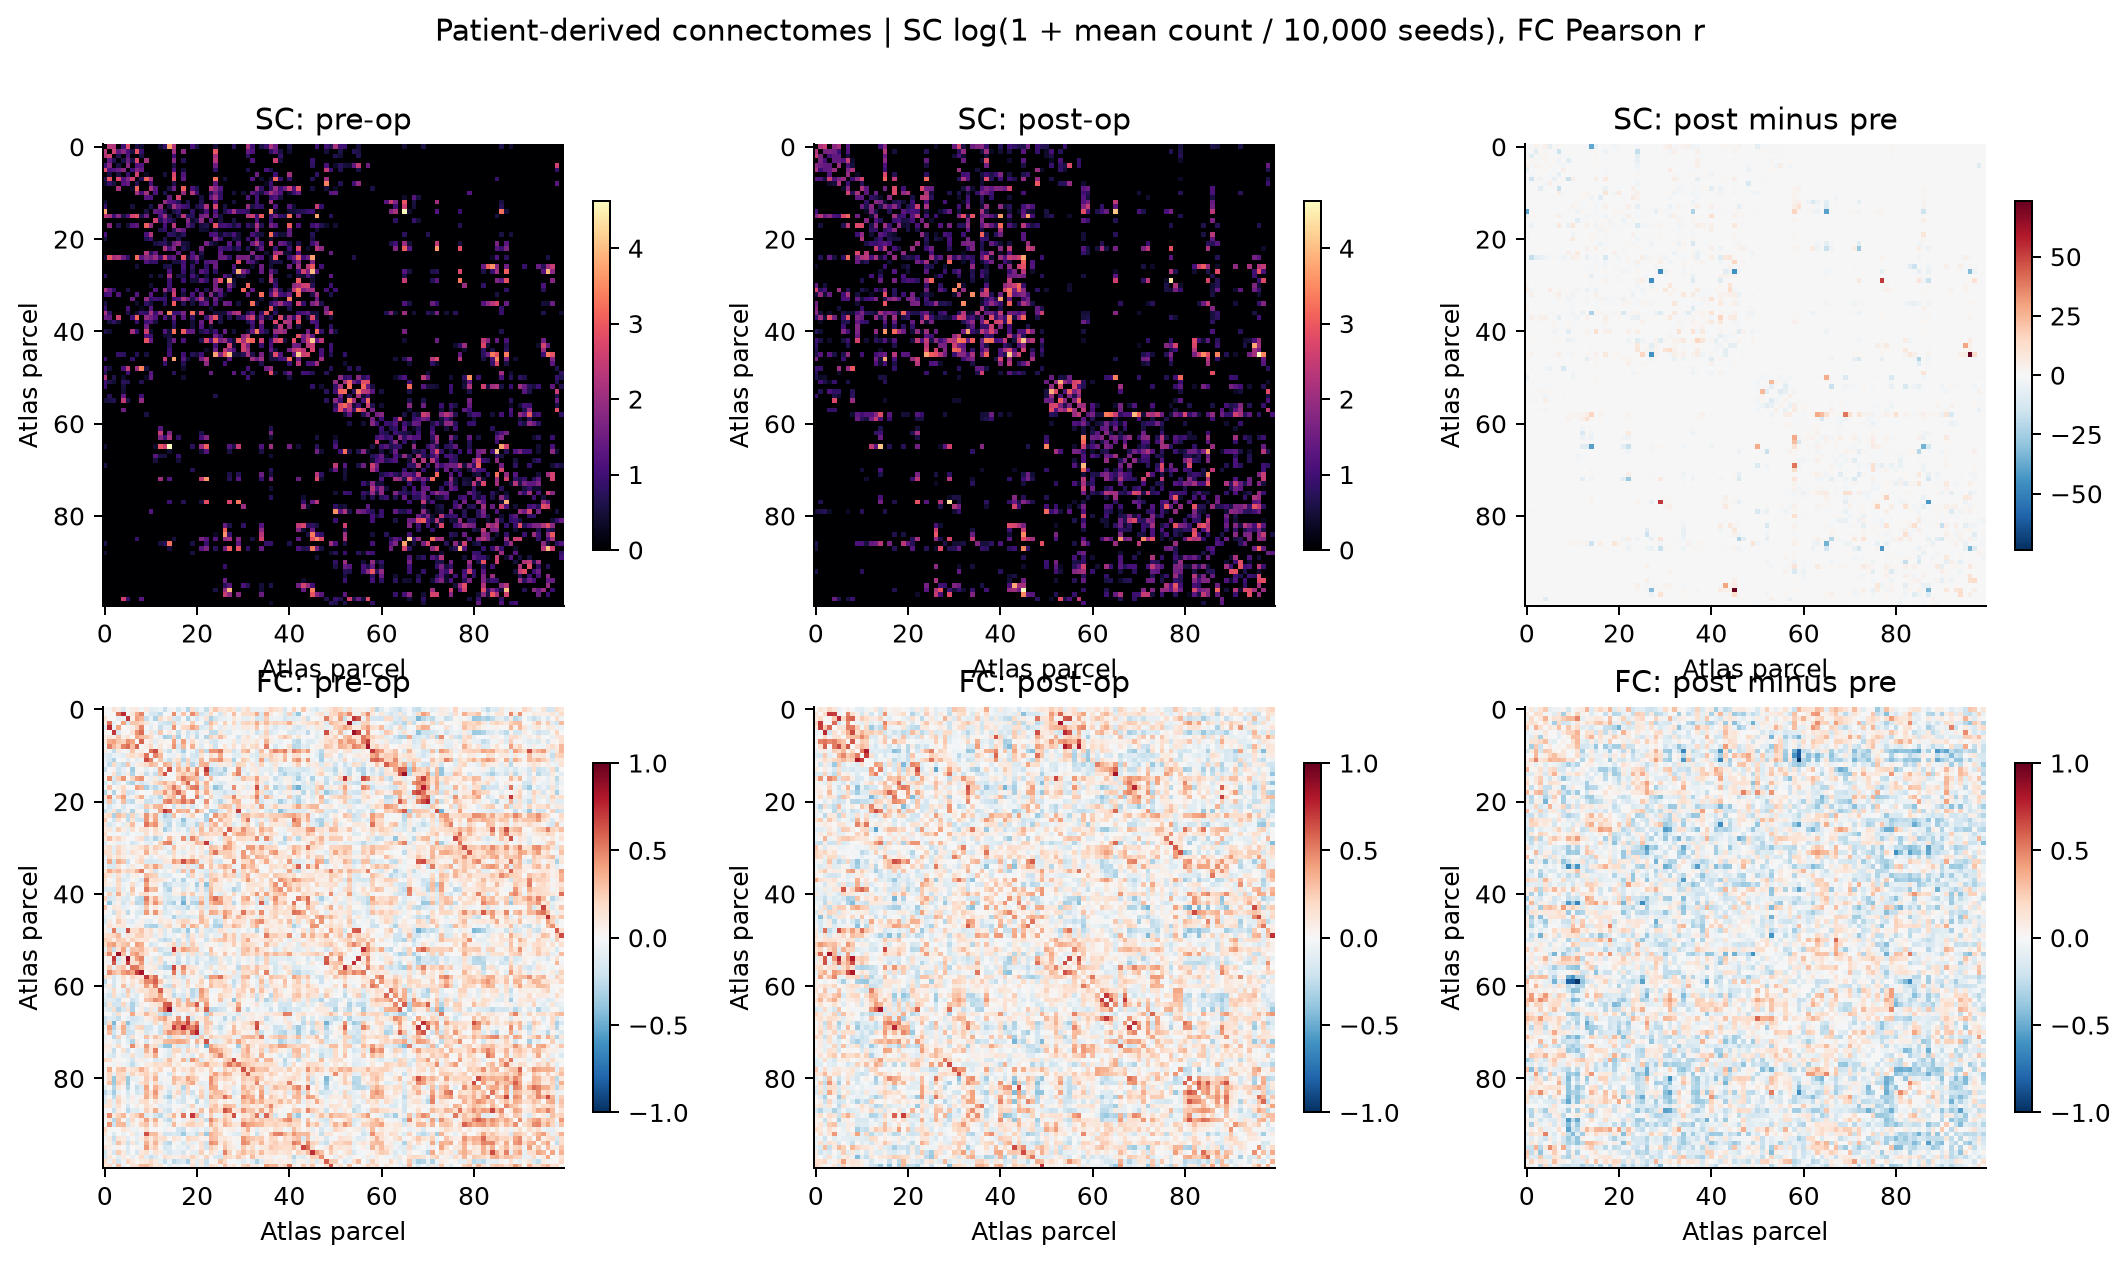
\includegraphics[width=\linewidth]{connectomes.png}
\caption{Fixed-order connectomes. SC pre/post displays use $\log(1+W)$ with own-consensus weights per 10,000 seeds; SC difference uses those same rate units. FC is signed Pearson correlation after the anatomical primary fit. Shared node identity does not remove registration and tracking bias.}\label{fig:matrices}\end{figure}

\subsection{BOLD correction and nuisance sensitivity}
Table~\ref{tab:boldqc} reports valid field coverage and signed shifts. All 100 parcels pass coverage checks in every processing variant; censoring remains exactly unchanged. No nonpositive Jacobians occur inside the reference brain mask. Anatomical overlays and slice views document approximate alignment (Fig.~\ref{fig:boldqc}); contrast differences, residual distortion and lesion-related misregistration remain possible.
\begin{table}[H]\centering\small\begin{tabular}{lrr}
\toprule
Quantity & Pre-op & Post-op \\
\midrule
BOLD readout time (s) & 0.01464 & 0.01464 \\
Alternative displacement scale & 0.761 & 0.761 \\
Reference brain with valid support (\%) & 96.206 & 95.16 \\
Signed shift: 1st percentile (vox) & -1.673 & -1.492 \\
Signed shift: 99th percentile (vox) & 1.15 & 1.15 \\
Nonpositive Jacobians in reference brain & 0 & 0 \\
\bottomrule
\end{tabular}

\caption{Static BOLD correction QC. Valid support requires field coverage, positive Jacobians and in-bounds coordinates across all frames. Shift percentiles use reference brain within source field support; values are signed raw PE-axis voxels.}\label{tab:boldqc}\end{table}
\begin{figure}[H]\centering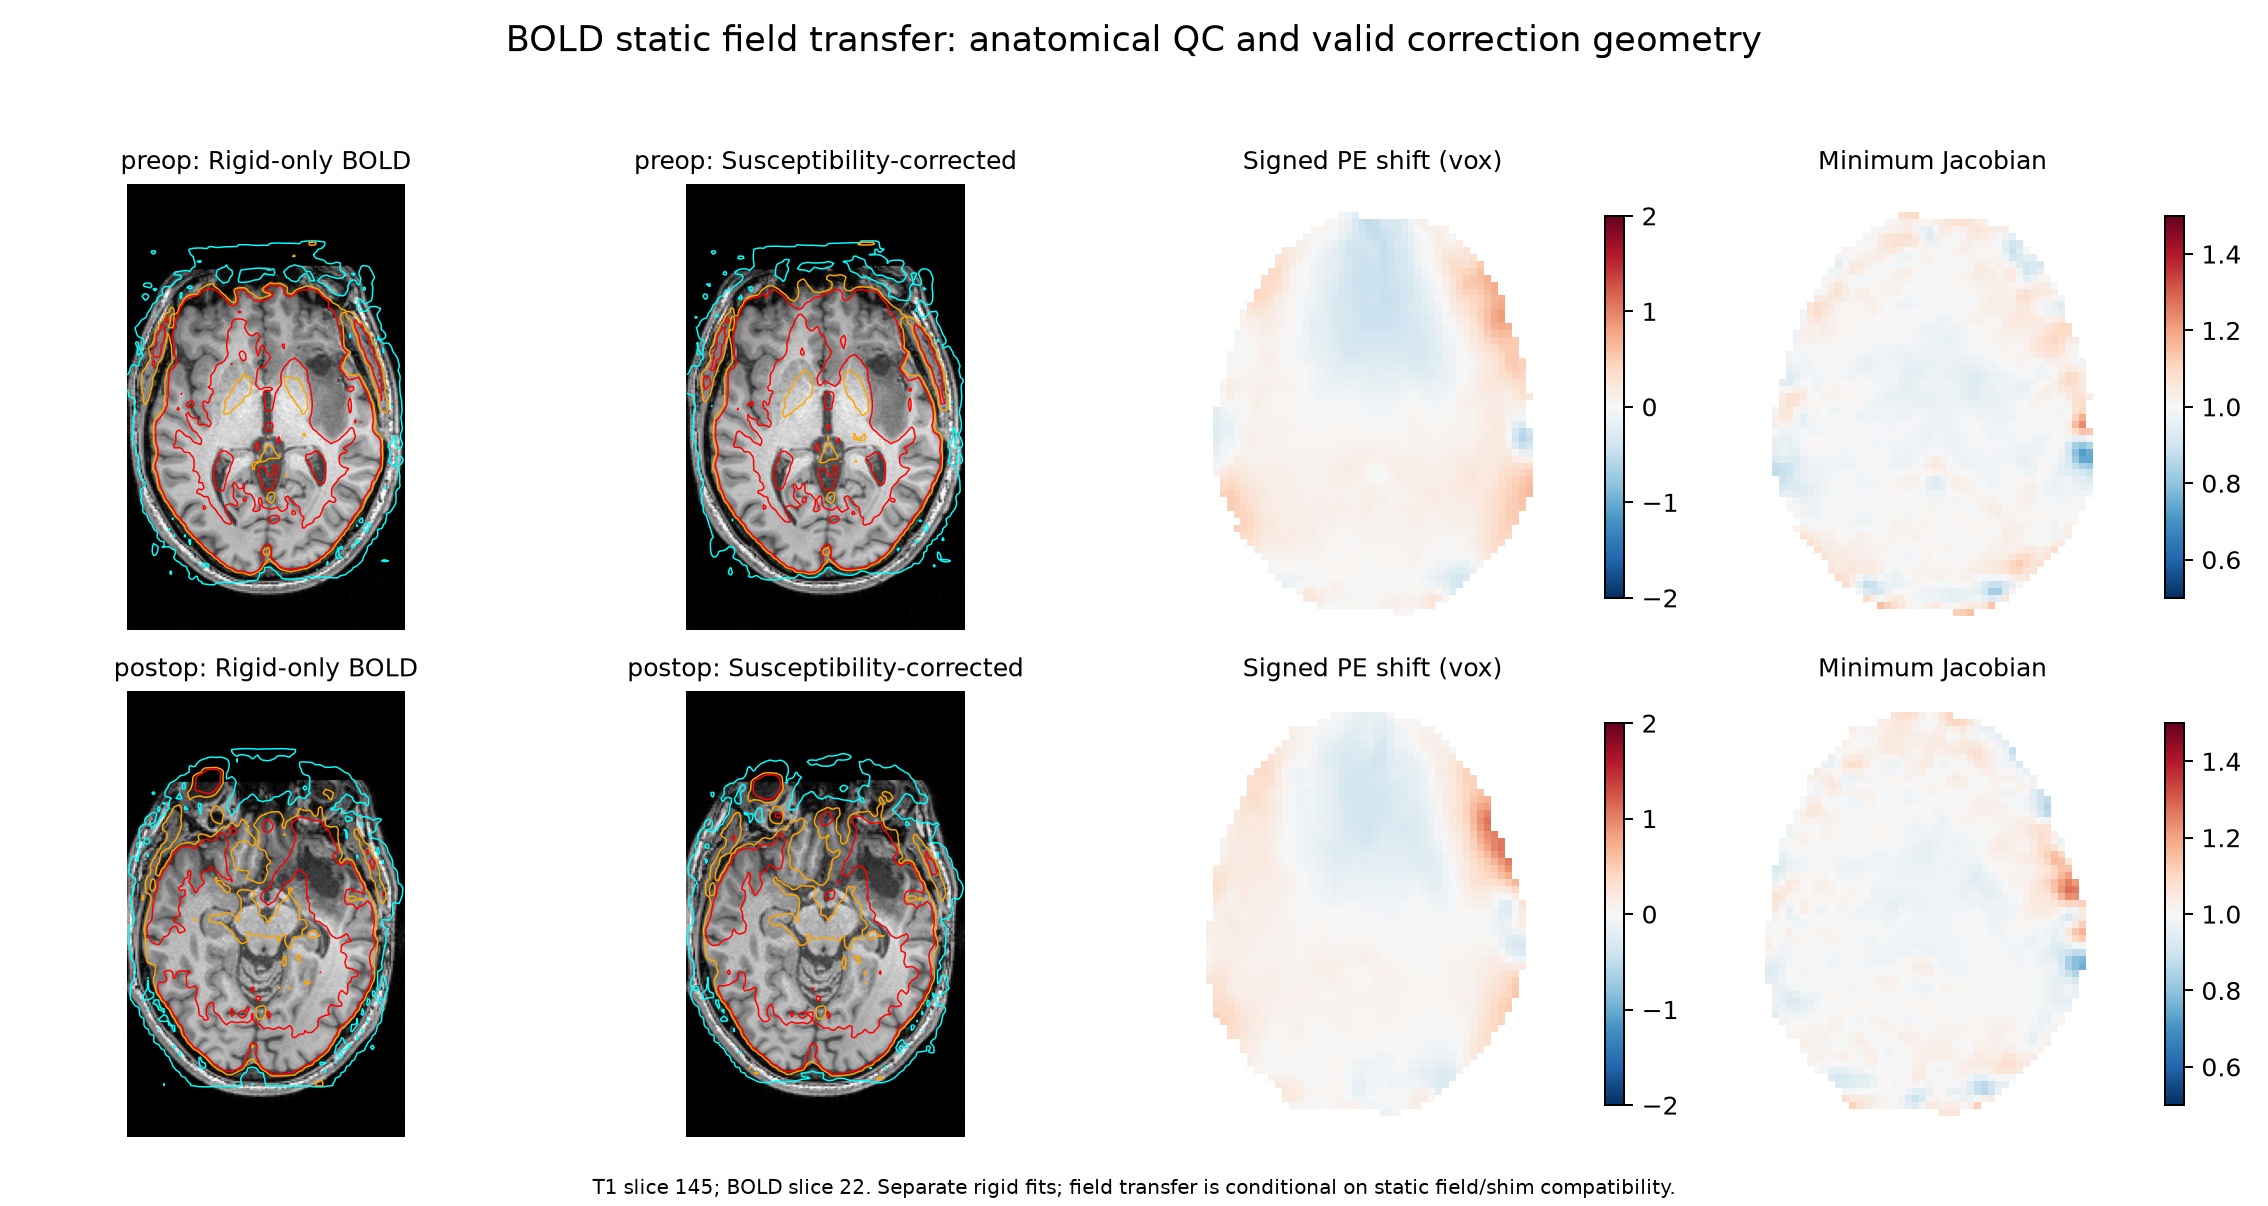
\includegraphics[width=\linewidth]{bold_distortion_qc.png}
\caption{BOLD reference contours over the same T1 slice before/after correction, each using its own rigid fit. Native BOLD shift and minimum-over-frames Jacobian are masked to valid support. Native reference/b0 slice sliders are available in notebook 02. These are QC views, not independent anatomical validation.}\label{fig:boldqc}\end{figure}

With the SAME anatomical five-PC recipe fitted to each BOLD package, rigid-only mean FC was \PreMeanFCOld{} and \PostMeanFCOld{}; the corrected pipeline gives \PreMeanFCPrimary{} and \PostMeanFCPrimary{}. With fixed common-consensus corrected SC, coupling changes from \PreCouplingOld{}/\PostCouplingOld{} to \PreCoupling{}/\PostCoupling{} (pre/post). The alternative timing scale gives mean FC \PreMeanFCAlt{}/\PostMeanFCAlt{} and coupling \PreCouplingAlt{}/\PostCouplingAlt{}. These two amplitude choices yield similar FC under refitted nuisance models; this does not establish robustness to field-transfer or physiological uncertainty (Table~\ref{tab:boldcomparison}, Fig.~\ref{fig:boldcomparison}).
\begin{table}[H]\centering\small\begin{tabular}{llrrr}
\toprule
Session & BOLD processing & Mean FC $r$ & SC--FC $\rho$ & FC weighted $E$ \\
\midrule
preop & Rigid only, matched denoising & 0.100 & 0.184 & 0.2215 \\
preop & Static field transfer & 0.087 & 0.188 & 0.2136 \\
preop & Alternative timing & 0.089 & 0.186 & 0.2149 \\
postop & Rigid only, matched denoising & 0.048 & 0.146 & 0.1961 \\
postop & Static field transfer & 0.046 & 0.146 & 0.1936 \\
postop & Alternative timing & 0.044 & 0.145 & 0.1929 \\
\bottomrule
\end{tabular}

\caption{BOLD processing sensitivity with identical 823-edge common-consensus SC support, 100 common nodes, motion estimates and censoring. FC weighted efficiency uses positive edges at density 0.20 and scale 1. All rows use retained-frame anatomical five-PC regression. Spatial sampling, masks and nuisance estimates are refitted.}\label{tab:boldcomparison}\end{table}
\begin{figure}[H]\centering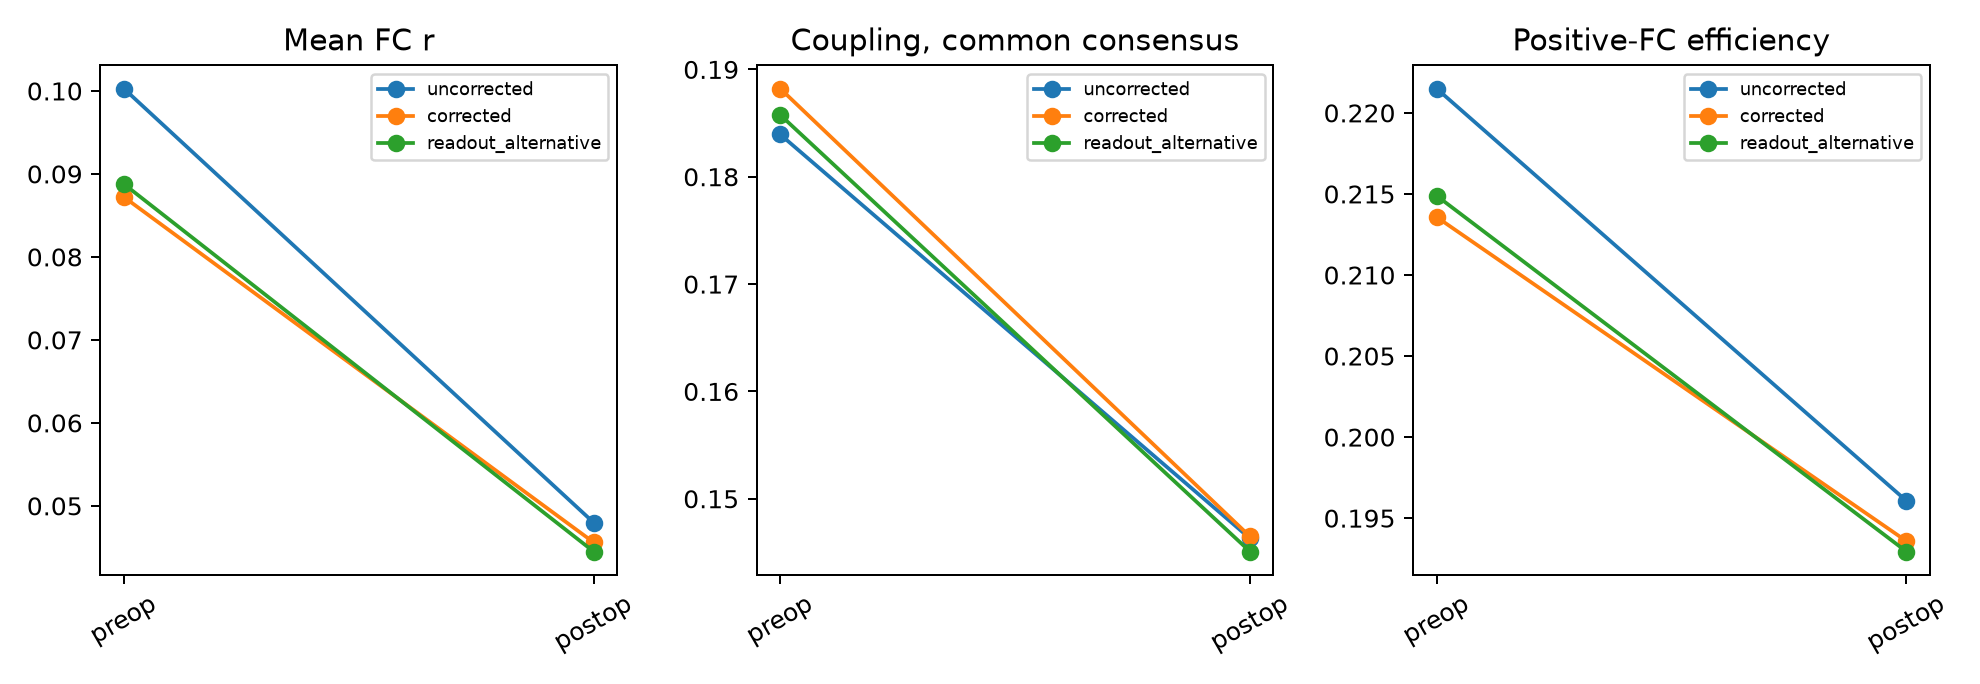
\includegraphics[width=\linewidth]{primary_sc_bold.png}
\caption{Rigid-only BOLD, static field transfer and alternative timing, all with the anatomical primary recipe. Lines connect descriptive case estimates. Historical noncortical-PC sensitivity is shown separately.}\label{fig:boldcomparison}\end{figure}

The separate historical noncortical component-swap diagnostic explains the earlier sensitivity (Table~\ref{tab:boldnuisance}). Holding postoperative ROI signals fixed at the previous version but refitting PCs reproduces most of the mean-FC shift. Conversely, corrected ROI signals with previous PCs give a mean close to the previous pipeline. Thus the postoperative shift cannot be described as the isolated effect of geometrical unwarping, improved neural measurement or surgery. The noncortical masks are not validated WM/CSF segmentations; the swaps diagnose model dependence and do not select a preferred biological estimate.
\begin{table}[H]\centering\small\begin{tabular}{llrr}
\toprule
ROI signals & Nuisance PCs & Mean FC pre $r$ & Mean FC post $r$ \\
\midrule
Previous & Previous & 0.365 & 0.272 \\
Previous & Refitted & 0.358 & 0.135 \\
Corrected & Previous & 0.363 & 0.268 \\
Corrected & Refitted & 0.360 & 0.133 \\
\bottomrule
\end{tabular}

\caption{Historical noncortical-PC diagnostic (not the current primary model): cross ROI signals and five nuisance PCs while holding motion, temporal design and censoring fixed. Only the all-previous and all-corrected rows are complete pipelines. The mixed rows are diagnostic counterfactual processing choices.}\label{tab:boldnuisance}\end{table}

\subsection{Mechanism of the postoperative PC sensitivity}
The historical PCA reconstruction reproduces each saved five-PC subspace to numerical precision. Thus neither a sign flip nor failure to reconstruct the earlier method explains the sensitivity. Postoperative noncortical membership changes from 11,054 to 9,335 EPI voxels (Dice 0.877); 2,109 old voxels are lost, 390 added, and 684 old voxels fail corrected field support. Preoperative Dice is 0.945. The minimum squared canonical correlation between the old/new five-PC subspaces, after base regression, is 0.350 postoperatively: they span materially different temporal directions.

The five-PC truncation is consequential (Table~\ref{tab:pccutoff}, Fig.~\ref{fig:pcmechanism}). On the same postoperative cortical signals, the old five PCs give mean FC 0.268 and remove 22.5\% of cortical-mean residual variance; the refitted five give 0.133 and remove 71.3\%. Old PC6 and new PC5 each associate strongly with the cortical mean after base regression (squared partial correlations 0.350 and 0.495). Their mutual partial correlation is only 0.331 in magnitude, so this is not a simple one-to-one PC swap. Including old PC6 drops mean FC to 0.156; ten old/refitted PCs give 0.102/0.101. These observations identify cutoff and subspace dependence, not an optimal number of components. Component variance fractions near ranks 5/6 are approximately 1.2--1.4\%; the findings do not demonstrate a numerical eigensolver failure.
\begin{table}[H]\centering\small\begin{tabular}{rrrrr}
\toprule
PCs & Old mean FC & Refit mean FC & Old partial $R^2$ & Refit partial $R^2$ \\
\midrule
4 & 0.277 & 0.272 & 0.151 & 0.178 \\
5 & 0.268 & 0.133 & 0.225 & 0.713 \\
6 & 0.156 & 0.102 & 0.657 & 0.790 \\
10 & 0.102 & 0.101 & 0.790 & 0.805 \\
\bottomrule
\end{tabular}

\caption{Postoperative PC-count diagnostic on identical corrected cortical signals. Partial $R^2$ refers to the cortical ROI mean after the base motion/DCT fit.}\label{tab:pccutoff}\end{table}
\begin{figure}[H]\centering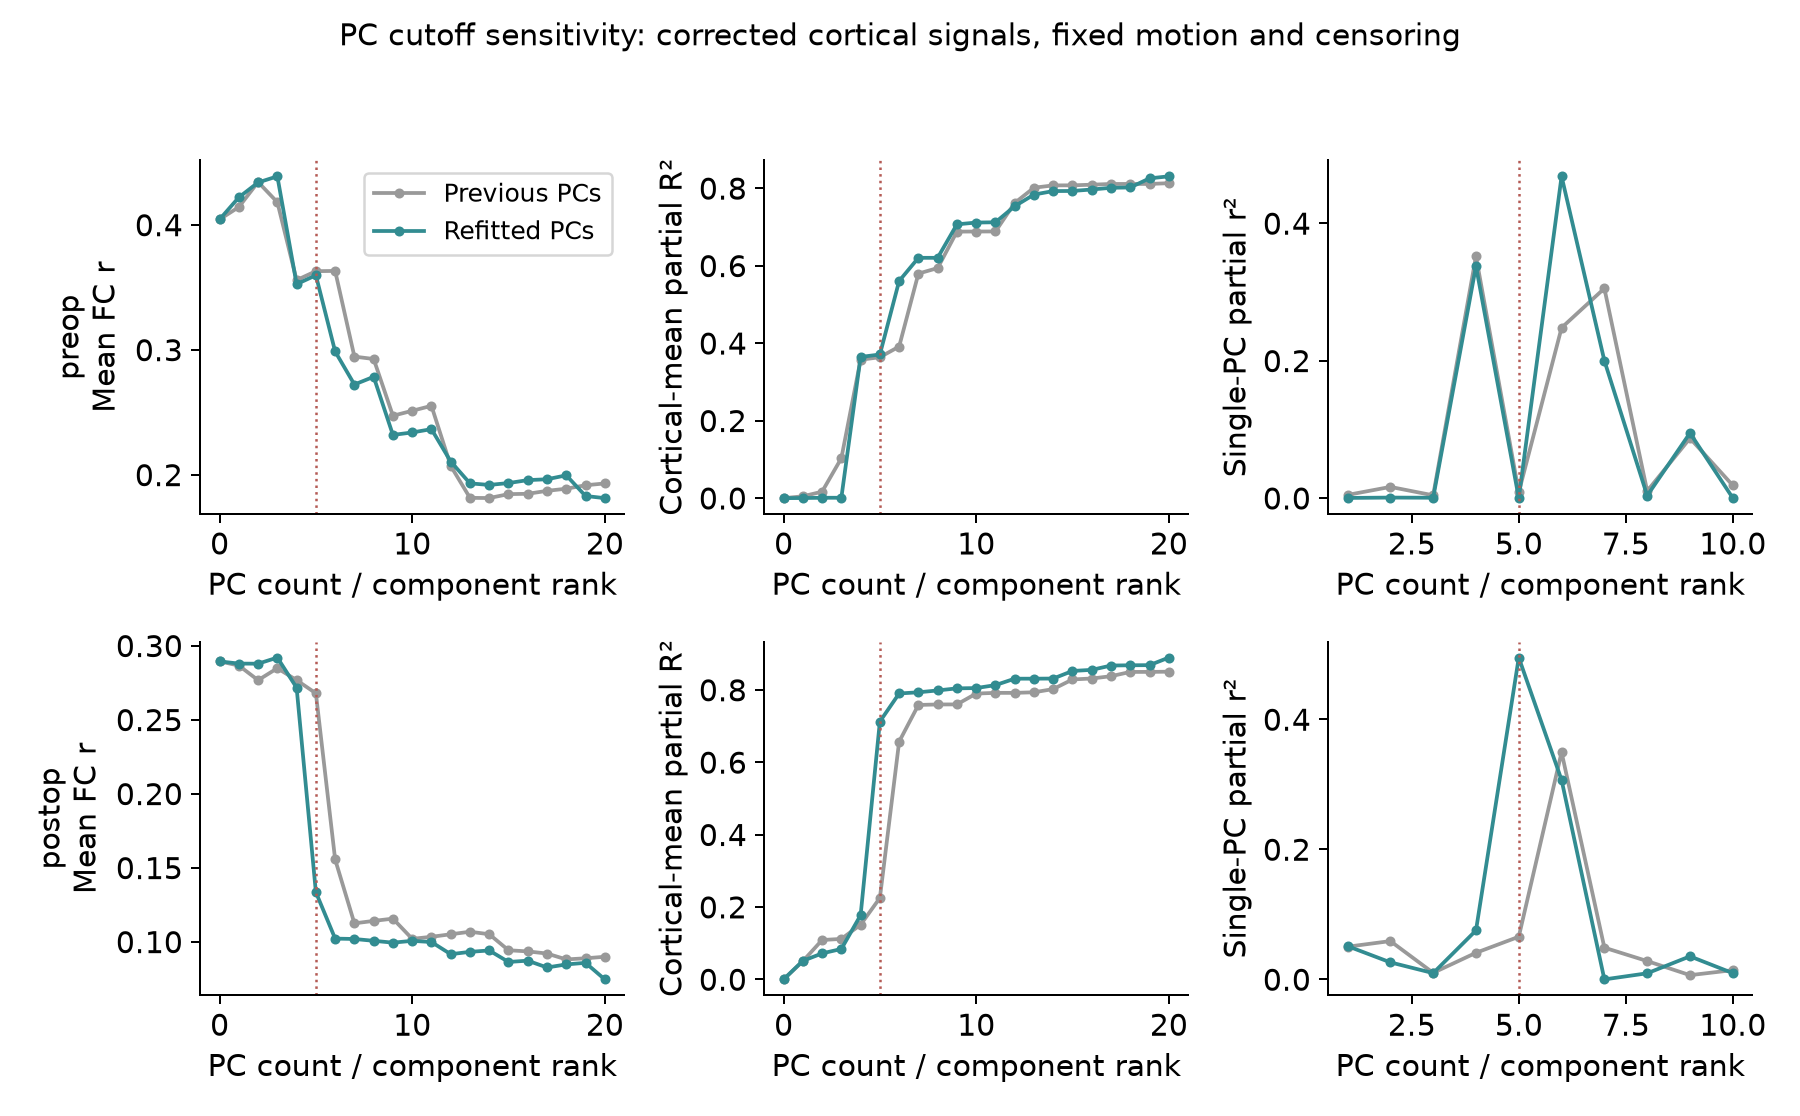
\includegraphics[width=\linewidth]{nuisance_pc_mechanism.png}
\caption{Cutoff sweeps and individual component associations after base motion/DCT regression. The dashed vertical line marks the historical five-PC choice. Squared correlations suppress arbitrary component signs and do not identify neural versus artifact variance.}\label{fig:pcmechanism}\end{figure}

The matched resampling control changes the interpretation of the earlier comparison (Table~\ref{tab:pcfactorial}). With the new postoperative mask, historical linear data give mean FC 0.254, cubic zero-field data 0.143 and cubic static-field data 0.133. With the mask intersection the corresponding values are 0.248, 0.150 and 0.144. Thus much of this diagnostic sensitivity appears even with zero susceptibility displacement. The same coordinate map with linear sampling reproduces historical interior-mask intensities with relative RMS error below $10^{-6}$ on five tested frames/session. Interpolation, masks and PC truncation interact; the remaining cubic zero-field/static-field difference includes field displacement and Jacobian modulation. We do not assign causal percentages to these interacting stages or identify the entire FC shift with susceptibility correction.
\begin{table}[H]\centering\small\begin{tabular}{llrrrr}
\toprule
Session & PCA image & Old mask & New mask & Old valid & Intersection \\
\midrule
preop & Linear, zero shift & 0.363 & 0.354 & 0.363 & 0.364 \\
preop & Cubic, zero shift & 0.359 & 0.353 & 0.359 & 0.364 \\
preop & Cubic, static field & 0.361 & 0.360 & 0.361 & 0.370 \\
postop & Linear, zero shift & 0.268 & 0.254 & 0.253 & 0.248 \\
postop & Cubic, zero shift & 0.226 & 0.143 & 0.179 & 0.150 \\
postop & Cubic, static field & 0.225 & 0.133 & 0.175 & 0.144 \\
\bottomrule
\end{tabular}

\caption{Mean FC with fixed corrected cortical signals and five PCs fitted to crossed images/masks. ``Old valid'' restricts the old mask to corrected field support; ``Intersection'' fixes overlapping mask membership on the common grid. These are diagnostic regressions, not twelve validated pipelines.}\label{tab:pcfactorial}\end{table}

\subsection{Anatomical WM/CSF denoising comparison}
The anatomical corrected masks contain 10,016/9,586 WM and 1,460/1,738 CSF voxels (pre/post). Their own mean target-class fractions exceed 0.996 and mean GM fractions are below 0.004; the historical corrected noncortical masks have mean GM fraction about 0.19 (Table~\ref{tab:nuisancemasks}). These are internal FAST-derived composition estimates, not independent accuracy measurements. Representative native and BOLD-projected masks are shown in Fig.~\ref{fig:nuisancemasks}; notebook 06 permits slice inspection.
\begin{table}[H]\centering\small\begin{tabular}{llrrrr}
\toprule
Session & Mask & EPI voxels & WM fraction & CSF fraction & GM fraction \\
\midrule
preop & Noncortical & 10508 & 0.721 & 0.056 & 0.194 \\
preop & WM & 10016 & 0.999 & 0.000 & 0.001 \\
preop & CSF & 1460 & 0.000 & 0.996 & 0.003 \\
postop & Noncortical & 9335 & 0.698 & 0.083 & 0.193 \\
postop & WM & 9586 & 0.998 & 0.000 & 0.002 \\
postop & CSF & 1738 & 0.000 & 0.997 & 0.003 \\
\bottomrule
\end{tabular}

\caption{Corrected BOLD masks and mean linearly sampled FAST partial-volume fractions. Native erosion precedes EPI resampling. Fractions need not sum to one where segmentation support is absent.}\label{tab:nuisancemasks}\end{table}
\begin{figure}[H]\centering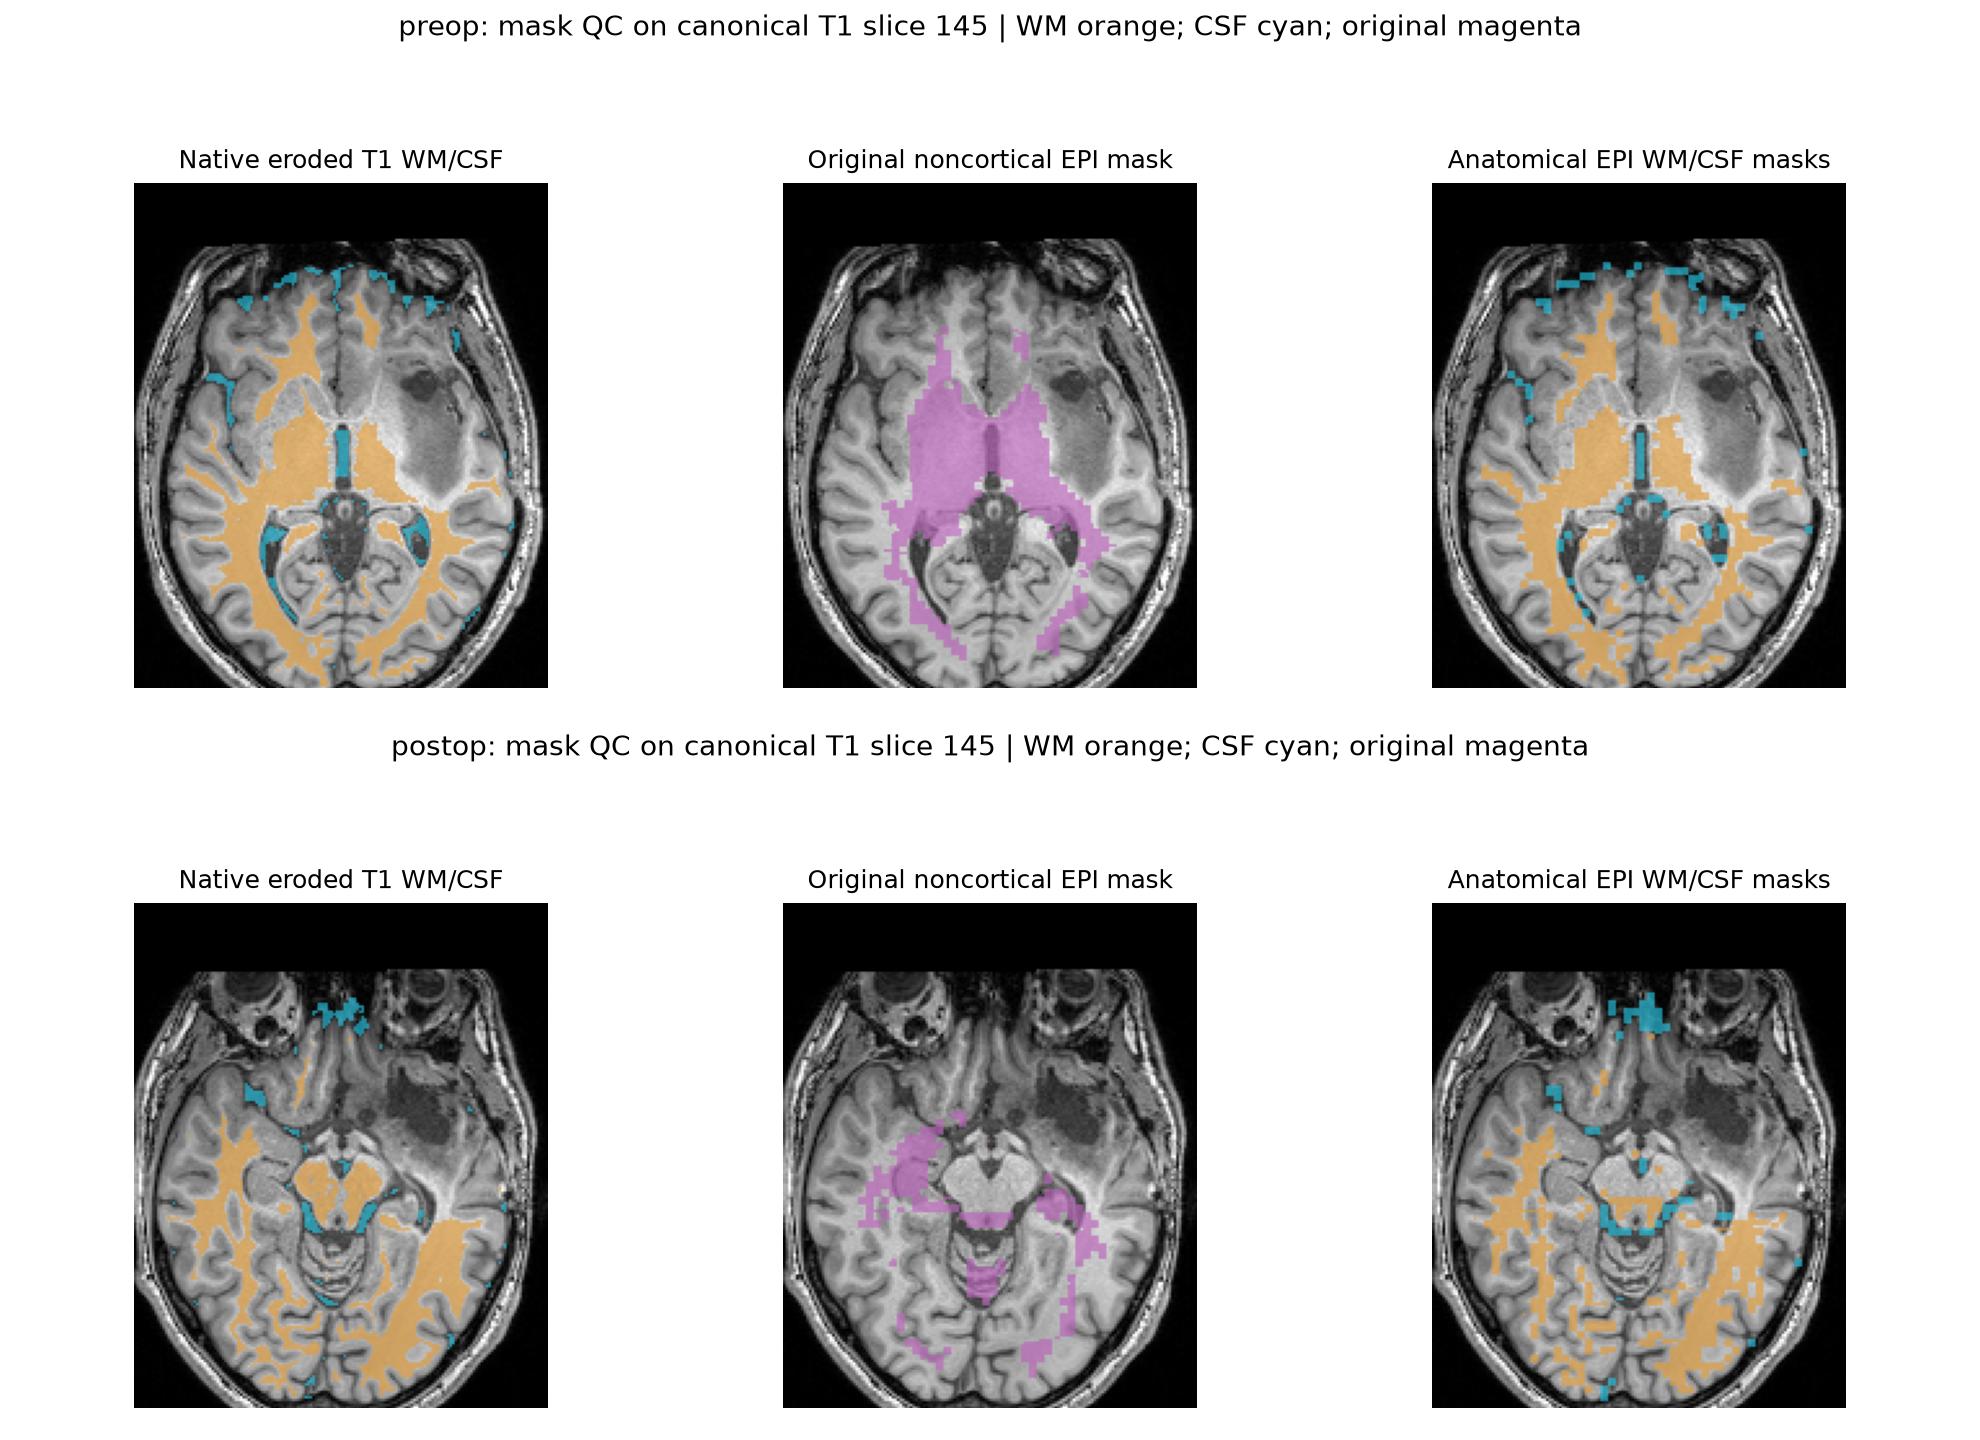
\includegraphics[width=\linewidth]{nuisance_mask_qc.png}
\caption{Session-native T1 mask QC at canonical axial slice 145. Native WM/CSF cores (left), historical noncortical EPI mask (centre) and anatomical EPI masks (right) are shown on the same T1 within each session. WM is orange, CSF cyan, historical mask magenta. Automatic segmentation and registration require expert review, especially near lesion/cavity and inferior cortex.}\label{fig:nuisancemasks}\end{figure}

Table~\ref{tab:nuisancemodels} compares six models on identical corrected signals, node sets and censored frames. Retained-frame anatomical five-PC regression gives mean FC \PreAnatFC{}/\PostAnatFC{} and SC--FC coupling \PreAnatCoupling{}/\PostAnatCoupling{}, compared with historical noncortical \PreLegacyFC{}/\PostLegacyFC{} and \PreLegacyCoupling{}/\PostLegacyCoupling{}. Applying the historical PCA recipe to the anatomical mask already gives 0.112/0.049: tissue selection makes a large difference before retained-frame temporal preprocessing. Separate WM5+CSF5 and tissue means yield further distinct estimates (Fig.~\ref{fig:nuisancemodels}).
\begin{table}[H]\centering\footnotesize\begin{tabular}{lrrrrrr}
\toprule
Model & FC pre & FC post & $\rho$ pre & $\rho$ post & df pre & df post \\
\midrule
Motion/DCT only & 0.404 & 0.289 & 0.101 & 0.110 & 112 & 116 \\
Original noncortical 5 PCs & 0.360 & 0.133 & 0.147 & 0.142 & 107 & 111 \\
Anatomical 5 PCs, raw fit & 0.112 & 0.049 & 0.189 & 0.133 & 107 & 111 \\
\textbf{Primary: anatomical 5 PCs} & 0.087 & 0.046 & 0.188 & 0.146 & 107 & 111 \\
WM5 + CSF5, retained fit & 0.049 & 0.033 & 0.221 & 0.124 & 102 & 106 \\
WM and CSF means & 0.078 & 0.060 & 0.140 & 0.101 & 110 & 114 \\
\bottomrule
\end{tabular}

\caption{Complete denoising alternatives on corrected BOLD. FC is upper-triangle mean Pearson $r$; $\rho$ is SC--FC Spearman correlation on the 823-edge common consensus; df is residual regression degrees of freedom. The bold row is the recommended primary; all other rows are sensitivity analyses. Historical main outputs are archived.}\label{tab:nuisancemodels}\end{table}
\begin{figure}[H]\centering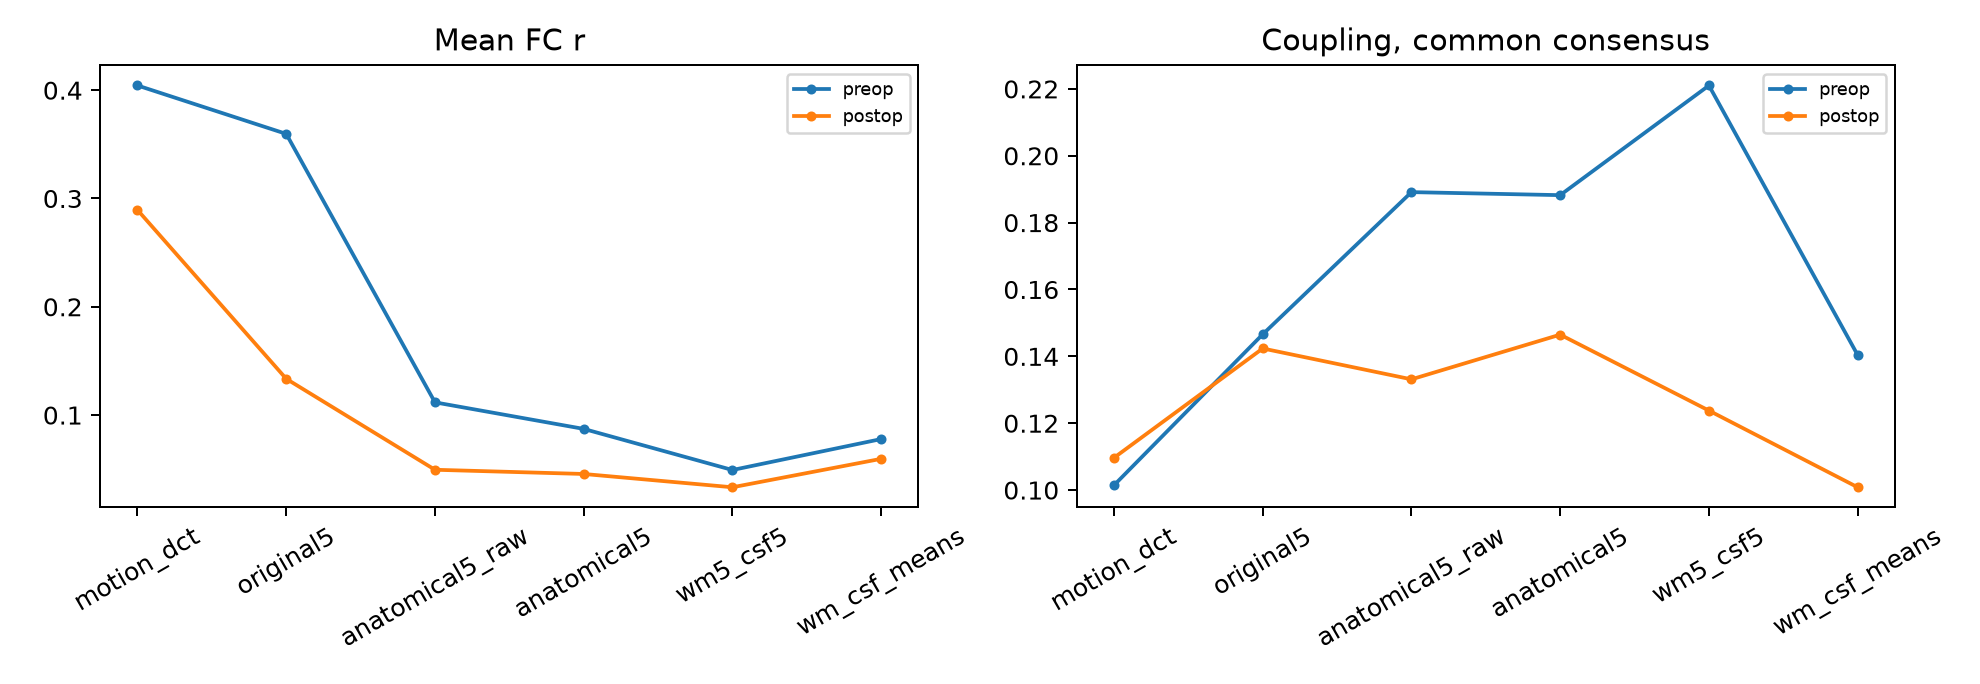
\includegraphics[width=\linewidth]{primary_sc_denoising.png}
\caption{Anatomical-mask alternatives change mean FC and coupling on the primary common-consensus SC population. Removal of shared cortical variance does not establish biological denoising quality. No model includes explicit global signal regression.}\label{fig:nuisancemodels}\end{figure}

The anatomical five-PC old/new BOLD comparison gives \PreAnatFCOld{}/\PreAnatFC{} preoperatively and \PostAnatFCOld{}/\PostAnatFC{} postoperatively. The postoperative package gap is approximately 0.0024, versus 0.1384 with historical five-PC regression. This reduction in processing dependence does not demonstrate neural validity: the anatomical model removes 90.7\%/90.3\% of cortical-mean residual variance and can remove neural as well as artifact covariance. Physiological recordings and independent segmentation/QC are unavailable. Whole-cortex mean FC is therefore strongly nuisance-model conditional even without explicit GSR.

For anatomical five-PC regression, varying the fraction threshold from 0.90 to 0.99 gives corrected mean FC 0.084--0.089 preoperatively and 0.045--0.048 postoperatively. Component count remains consequential (two PCs: 0.257/0.118; ten: 0.069/0.044 at threshold 0.95). Stricter FD censoring with PCA refitting gives 0.108/0.041, common-consensus coupling \PreStrictCoupling{}/\PostStrictCoupling{} and only 29/57 residual degrees of freedom. The across-session mean decrease occurs across these tested models, but its magnitude, graph weights and coupling depend on the nuisance model. Under primary common-consensus SC, both point contrasts are negative (\PrimarySCDelta{} and \StrictSCDelta{}). The historical seed-160 own-support contrasts instead reverse sign (0.210 to 0.189 versus 0.156 to 0.168). Support choice remains consequential; the new point estimates do not settle biological direction. The matched investigation in Section~\ref{sec:censoringresults} separates this duration/refitting sensitivity; absent physiological ground truth prevents a surgery-effect or neural-decline conclusion. FC retains the recommended anatomical fit; primary SC and coupling now follow Section~\ref{sec:primaryscmethods}. Conditional FC network intervals remain unchanged; preceding main FC is archived.

A sweep of 0--20 retained-frame anatomical PCs directly audits the recommended cutoff (Table~\ref{tab:primarycount}, Fig.~\ref{fig:primarycount}). Adjacent postoperative 4/5/6-PC means are 0.0477/0.0456/0.0449, without the large historical cutoff jump; preoperative means are 0.0864/0.0872/0.0721. Preoperative count dependence remains appreciable. This supports five as a usable fixed budget, not an optimized count or proof of neural preservation. We retain the full sweep rather than selecting a count from coupling or behavioural outcomes.
\begin{table}[H]\centering\small\begin{tabular}{rrrrr}
\toprule
PCs & FC pre & FC post & $\rho$ pre & $\rho$ post \\
\midrule
2 & 0.2570 & 0.1178 & 0.146 & 0.128 \\
4 & 0.0864 & 0.0477 & 0.189 & 0.144 \\
5 & 0.0872 & 0.0456 & 0.188 & 0.146 \\
6 & 0.0721 & 0.0449 & 0.196 & 0.144 \\
10 & 0.0688 & 0.0445 & 0.203 & 0.127 \\
\bottomrule
\end{tabular}

\caption{Anatomical PC-count sensitivity at PVE 0.95 and FD 0.5 mm, with masks, cortical signals and censoring fixed. Five PCs is the frozen primary recommendation.}\label{tab:primarycount}\end{table}
\begin{figure}[H]\centering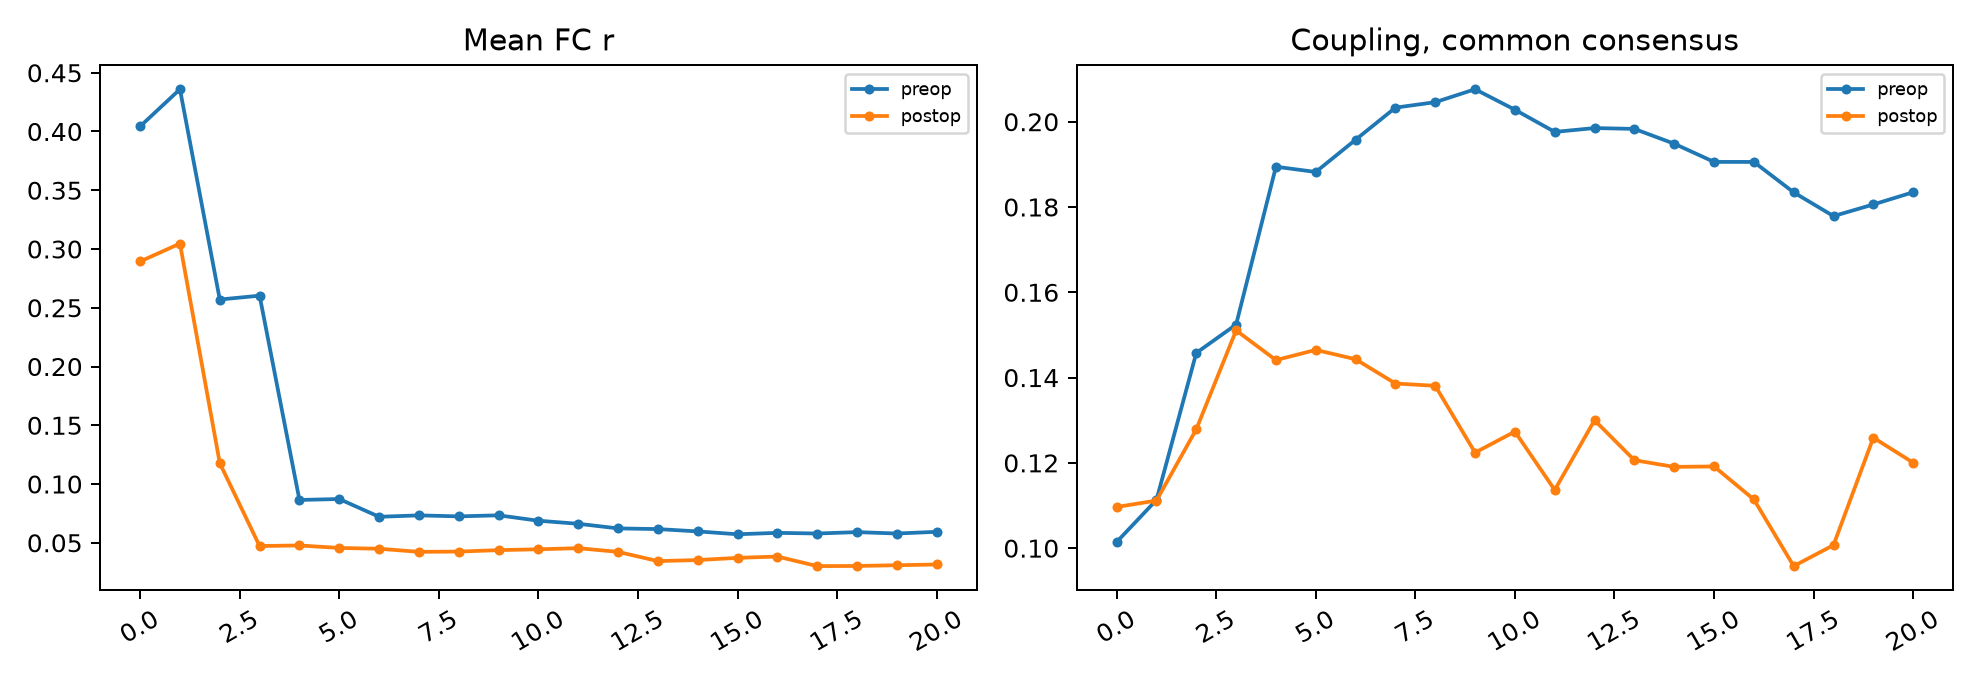
\includegraphics[width=\linewidth]{primary_sc_pc_count.png}
\caption{Wider anatomical-PC count sweep on corrected BOLD. The fixed primary budget is five PCs, not a fitted optimum; coupling uses common-consensus SC. All displayed fits pass the residual-df guard.}\label{fig:primarycount}\end{figure}

\subsection{Primary reliability-based SC results}\label{sec:primaryscresults}
Own consensus retains 1,160 pre-op and 1,163 post-op edges; their intersection contains 823 edges. The retained own-support mean assignments are 15,782.4/15,290.4 per 30,000 attempted seeds. These averages are neither integer pooled counts nor the historical seed-160 yields in Table~\ref{tab:qc}. Primary common-support coupling is \PreCoupling{}/\PostCoupling{}, giving $\Delta=\PrimarySCDelta{}$. Strict FD0.3 with full PCA/regression refitting gives \PreStrictCoupling{}/\PostStrictCoupling{}, $\Delta=\StrictSCDelta{}$ (Table~\ref{tab:primaryscchoice}). Own-consensus coupling instead gives $\Delta=-0.00257/+0.02363$ for primary/strict FC. Averaging without support filtering adds many rarely detected edges (2,581/2,688), producing yet another contrast. We select neither a threshold nor a weight rule to obtain these signs.
\begin{table}[H]\centering\scriptsize\setlength{\tabcolsep}{3pt}\begin{tabular}{lrrrrrr}
\toprule
SC population & Pre $n$ & Post $n$ & $\rho_P$ pre & $\rho_P$ post & $\Delta_P$ & $\Delta_S$ \\
\midrule
Historical single run, own & 1515 & 1559 & 0.2101 & 0.1894 & -0.0207 & +0.0111 \\
Unfiltered repeat mean, own & 2581 & 2688 & 0.2366 & 0.2386 & +0.0021 & +0.0344 \\
80\% consensus, own & 1160 & 1163 & 0.1893 & 0.1868 & -0.0026 & +0.0236 \\
\textbf{Primary coupling: common} & 823 & 823 & 0.1882 & 0.1465 & -0.0417 & -0.0342 \\
\bottomrule
\end{tabular}

\caption{Primary and complementary SC populations, with unchanged anatomical FC. $P$ denotes FD0.5 and $S$ full-refit FD0.3. Graphs use own 80\% consensus; paired coupling uses common 80\% consensus. All alternative settings remain exported.}\label{tab:primaryscchoice}\end{table}
\begin{figure}[H]\centering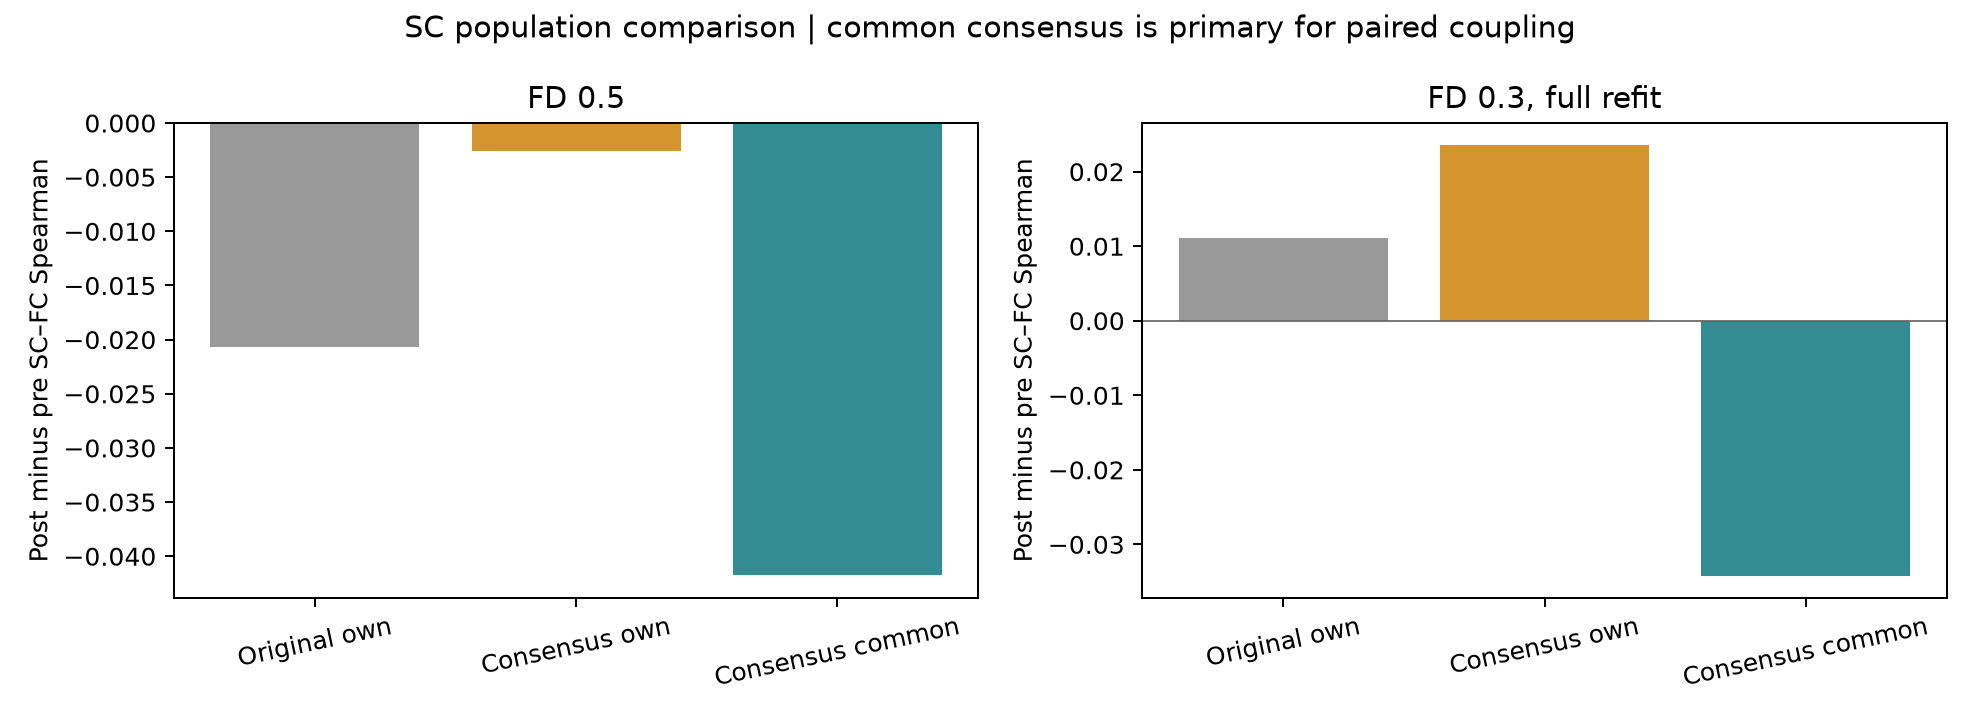
\includegraphics[width=\linewidth]{primary_sc_choice.png}
\caption{Changing the SC population changes longitudinal coupling. A common repeat-consensus population eliminates the original point-estimate sign reversal, without demonstrating biological direction or robustness to all sampling choices.}\label{fig:primaryscchoice}\end{figure}

Re-ranking the four ordered FC fits on this fixed 823-edge population gives contrasts $-0.04173$, $-0.02182$, $-0.03454$ and $-0.03424$ (Table~\ref{tab:primaryscdecomp}). There is no sign reversal in these point estimates; the strict-minus-primary shift is $+0.00749$. Current edge and network rank accounting is separately exported in \path{results/primary_sc}; its terms sum exactly to these new contrasts and do not inherit the historical $R=+0.03186$ decomposition.
\begin{table}[H]\centering\small\begin{tabular}{lrrr}
\toprule
Ordered FC fit & $\rho$ pre & $\rho$ post & $\Delta$ \\
\midrule
Primary: own frames/fit & 0.1882 & 0.1465 & -0.0417 \\
Strict frames: fixed primary fit & 0.1505 & 0.1286 & -0.0218 \\
+ refit regression, fixed PCs & 0.1602 & 0.1257 & -0.0345 \\
+ refit tissue PCA (strict pipeline) & 0.1608 & 0.1265 & -0.0342 \\
\bottomrule
\end{tabular}

\caption{Ordered diagnostic re-evaluated on primary common-consensus SC. Every row uses the same 823 edges; weights differ between sessions. Rows diagnose computational dependencies, not causal neural effects.}\label{tab:primaryscdecomp}\end{table}

All six saved 200-draw matched FC protocols have also been evaluated on the primary SC reference (Table~\ref{tab:primaryscmatched}). Every median is negative, yet five of six conditional central spreads cross zero. Strict duration+FD matching gives $-0.04797$ [$-0.08979,-0.01587$], while adding acquisition-half matching gives $-0.02217$ [$-0.05572,+0.00908$]. A negative spread in one conditional design is not a confidence interval or evidence of a surgery effect. These controls vary FC sampling at fixed consensus SC. Section~\ref{sec:jointresults} now crosses seed and FC sampling under the primary policy; scan/model uncertainty remains unestimated.
\begin{table}[H]\centering\small\begin{tabular}{llrr}
\toprule
Pool & Matching & Median $\Delta$ & Conditional 95\% spread \\
\midrule
Primary & Duration & -0.0335 & [-0.1029, +0.0442] \\
Primary & Duration + FD & -0.0346 & [-0.1280, +0.0498] \\
Primary & Duration + FD + half & -0.0389 & [-0.1092, +0.0368] \\
Strict & Duration & -0.0419 & [-0.0822, +0.0007] \\
Strict & Duration + FD & -0.0480 & [-0.0898, -0.0159] \\
Strict & Duration + FD + half & -0.0222 & [-0.0557, +0.0091] \\
\bottomrule
\end{tabular}

\caption{Primary common-consensus SC under full nuisance refitting, 68 frames per session and 200 draws per protocol. Conditional 2.5/97.5 percentiles describe the saved sampling design, not participant or treatment uncertainty.}\label{tab:primaryscmatched}\end{table}

\subsection{Primary fixed-duration FC stability results}\label{sec:primaryfcresults}
The observed common-support coupling is unchanged: $0.18822\rightarrow0.14649$, $\Delta=-0.04173$. All 200 primary subsets per session pass the feasibility guard: 97 distinct eligible frames, design rank 39 and 58 algebraic residual directions. The primary crossed-grid median change is $\PrimaryFCMedian{}$, with range $[\PrimaryFCLow{},\PrimaryFCHigh{}]$ (Table~\ref{tab:primaryfc}; Fig.~\ref{fig:primaryfc}). Conditional variance shares are SC \PrimarySCShare{}\%, FC \PrimaryFCShare{}\% and interaction \PrimaryInteractionShare{}\%. These shares compare only the implemented perturbations. The 4.236\% positive-cell fraction is a descriptive grid proportion, not a posterior probability or $p$-value.
\begin{table}[H]\centering\small\begin{tabular}{lrr}
\toprule
Frames / design & Median & Conditional range \\
\midrule
97, block 10, refit (primary) & -0.04694 & [-0.10261, +0.00832] \\
97, block 10, frozen & -0.04334 & [-0.07973, -0.00297] \\
97, block 10, coef. & -0.04636 & [-0.09917, +0.00794] \\
97, block 5, refit & -0.04232 & [-0.10014, +0.00938] \\
97, block 20, refit & -0.04278 & [-0.09486, +0.01833] \\
73, block 10, refit & -0.03519 & [-0.10387, +0.06171] \\
116, block 10, refit & -0.04918 & [-0.09209, -0.00799] \\
97, block 10, SC reselected & -0.05003 & [-0.10780, +0.00280] \\
\bottomrule
\end{tabular}

\caption{Recommended primary stability design and selected sensitivities. Every new design has 500 SC draws and 200 paired eligible FC draws; values are coupling-change medians and raw conditional 2.5/97.5 percentiles. Common retained counts are 73, 97 or 116 per session. ``Refit'' includes all nuisance training; ``coef.'' fixes PC scores. These are not full-run confidence intervals.}\label{tab:primaryfc}\end{table}
\begin{figure}[H]\centering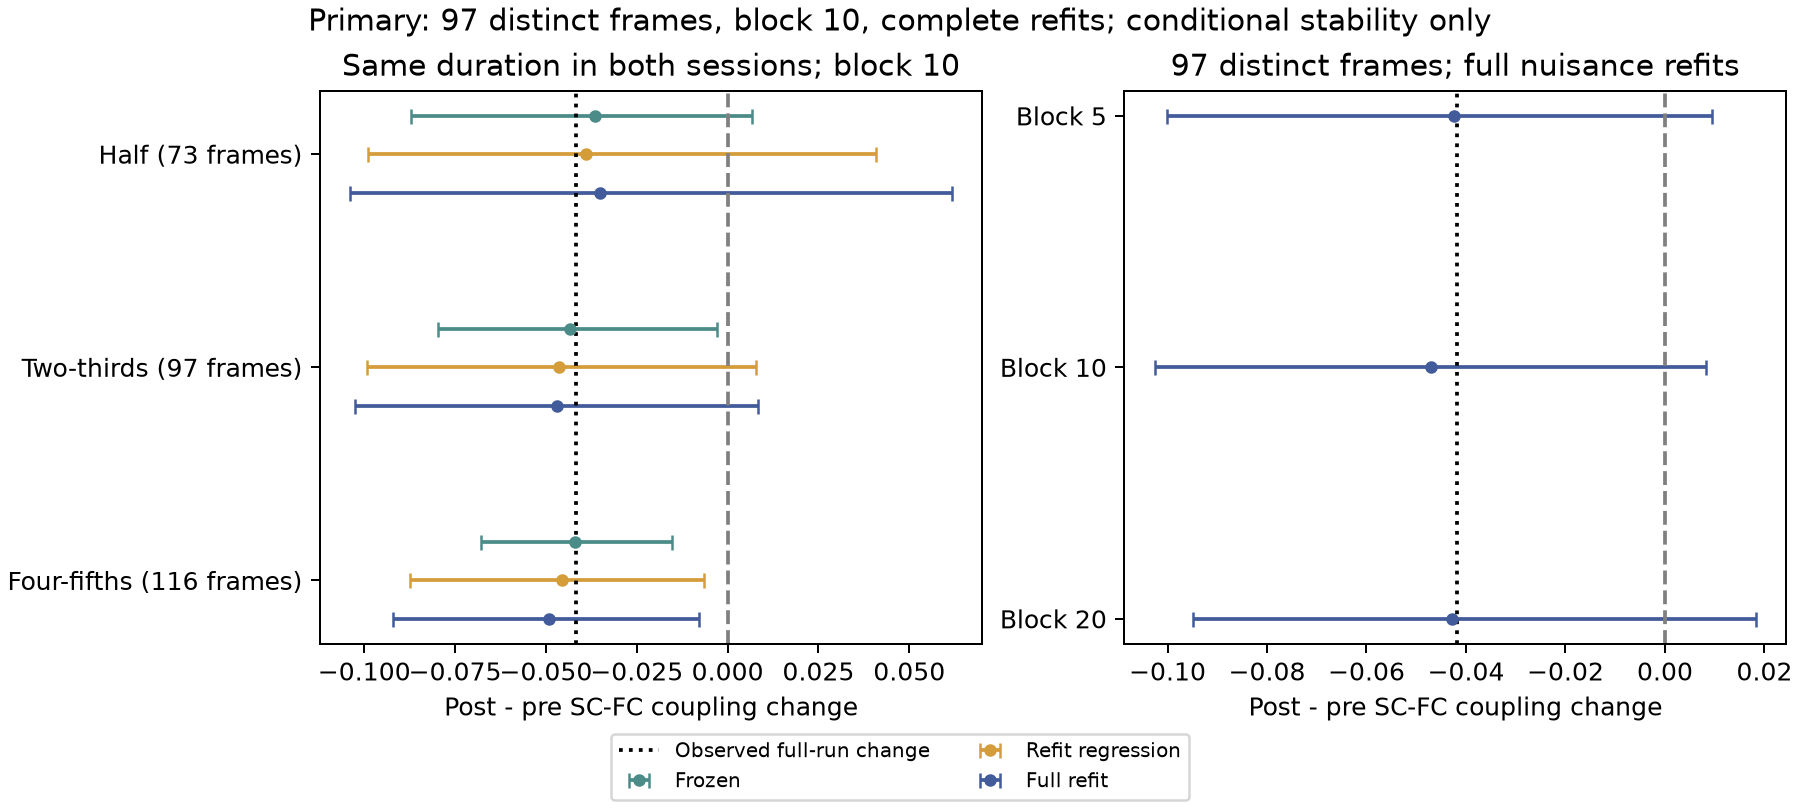
\includegraphics[width=\linewidth]{primary_fc_joint.png}
\caption{Fraction, nuisance training and block-length sensitivities on fixed common SC support. The dotted line is the unchanged observed full-run change; centers summarize subsets. Fractions are relative to the smaller 146-frame pool.}\label{fig:primaryfc}\end{figure}

At 97 frames and ten-frame blocks the frozen range $[-0.07973,-0.00297]$ is negative, whereas coefficient-only and full-refit ranges cross zero. Five- and twenty-frame complete refits also cross zero. At 73 frames the full-refit range widens to $[-0.10387,+0.06171]$; at 116 frames it narrows to $[-0.09209,-0.00799]$. Higher retained fractions approach the observed estimator and are not independent confirmation of its sign. Reselecting SC support gives $[-0.10780,+0.00280]$. Thus the recommendation is based on the estimator and sampling target, not a sign or narrow interval. Primary draws match retained duration, but do not match motion distributions; the previous 68-frame FD/run-half controls remain complementary sensitivities in Sections~\ref{sec:jointresults} and~\ref{sec:refitresults}. They use a different target and cannot calibrate the 97-frame ranges.

\subsection{Sensitivity: joint SC and FC bootstrap/matched results}\label{sec:jointresults}
The recommended primary point contrast remains $-0.04173$; the strict point contrast remains $-0.03424$. At fixed 823-edge support, the SC-only primary anchor has median $-0.04217$ and central range $[-0.04934,-0.03596]$. Crossing SC with full-primary ten-frame block FC sampling gives median $\JointPrimaryMedian{}$ and range $[\JointPrimaryLow{},\JointPrimaryHigh{}]$ (Table~\ref{tab:jointsources}). Full strict block sampling gives $\JointStrictMedian{}$ $[\JointStrictLow{},\JointStrictHigh{}]$. Both joint ranges cross zero. The full-primary finite-grid variance is \JointPrimarySCShare{}\% SC main effect, \JointPrimaryFCShare{}\% FC main effect and \JointPrimaryInteractionShare{}\% interaction. Thus seed sampling of the 20-run mean is much smaller than FC sampling in this conditional experiment; these shares do not rank unmeasured acquisition or model errors.
\begin{table}[H]\centering\small\begin{tabular}{llrrr}
\toprule
Full-run FC & Perturbation & Median $\Delta$ & Conditional 95\% range & SD \\
\midrule
Primary & SC only & -0.0422 & [-0.0493, -0.0360] & 0.0035 \\
Primary & FC only & -0.0404 & [-0.0829, +0.0146] & 0.0264 \\
Primary & joint & -0.0405 & [-0.0839, +0.0158] & 0.0265 \\
Strict & SC only & -0.0344 & [-0.0423, -0.0263] & 0.0041 \\
Strict & FC only & -0.0292 & [-0.0824, +0.0326] & 0.0297 \\
Strict & joint & -0.0298 & [-0.0844, +0.0315] & 0.0298 \\
\bottomrule
\end{tabular}

\caption{Full-run, fixed-823-edge support: source-specific anchors and joint temporal/seed resampling. Blocks have ten original frames; nuisance fits remain fixed. SC-only uses observed full-run FC. Central ranges are conditional percentiles, not clinical confidence intervals.}\label{tab:jointsources}\end{table}
\begin{table}[H]\centering\scriptsize\begin{tabular}{llrr}
\toprule
Full-run FC & Support & Pre-op $\rho$: median [range] & Post-op $\rho$: median [range] \\
\midrule
Primary & fixed & 0.1756 [0.1412, 0.2098] & 0.1343 [0.1022, 0.1724] \\
Primary & reselected & 0.1772 [0.1372, 0.2157] & 0.1334 [0.0974, 0.1741] \\
Strict & fixed & 0.1488 [0.0988, 0.1948] & 0.1174 [0.0766, 0.1563] \\
Strict & reselected & 0.1424 [0.0935, 0.1901] & 0.1165 [0.0734, 0.1607] \\
\bottomrule
\end{tabular}

\caption{Per-session joint coupling ranges for full-run ten-frame blocks. Paired contrast ranges are computed from the joint draws, not by subtracting these marginal endpoints. Support reselection changes the connection population.}\label{tab:jointsessions}\end{table}

All six fully refitted matched protocols have negative joint medians, while five of six fixed-support central ranges cross zero (Table~\ref{tab:jointfixed}; Fig.~\ref{fig:jointranges}). Strict duration+FD gives $\JointStrictMotionMedian{}$ $[\JointStrictMotionLow{},\JointStrictMotionHigh{}]$, with \JointStrictMotionPositive{}\% positive grid cells. Adding run-half matching gives $\JointStrictHalfMedian{}$ $[\JointStrictHalfLow{},\JointStrictHalfHigh{}]$, with \JointStrictHalfPositive{}\% positive cells. The former fixed-SC FD-matched positive fraction was zero; allowing uncertain SC weights makes a small fraction positive. This conditional negative central range does not establish a surgical direction, especially given the change after coarse temporal matching and the constant strict pre-op matched FC. FC main-effect shares are about 94--99\% across all fixed-support protocols, with smaller SC and interaction shares.
\begin{table}[H]\centering\scriptsize\setlength{\tabcolsep}{3pt}\begin{tabular}{lrrrrr}
\toprule
FC design & Median $\Delta$ & Conditional 95\% range & $\Delta>0$ (\%) & SC (\%) & FC (\%) \\
\midrule
Full primary, block 10 & -0.0405 & [-0.0839, +0.0158] & 9.16 & 1.5 & 98.2 \\
Full strict, block 10 & -0.0298 & [-0.0844, +0.0315] & 17.49 & 1.5 & 98.2 \\
Primary: duration & -0.0337 & [-0.1039, +0.0432] & 20.61 & 0.5 & 99.2 \\
Primary: duration + FD & -0.0354 & [-0.1286, +0.0499] & 17.82 & 0.4 & 99.3 \\
Primary: duration + FD + half & -0.0392 & [-0.1105, +0.0368] & 17.90 & 0.5 & 99.1 \\
Strict: duration & -0.0427 & [-0.0855, +0.0005] & 2.61 & 3.1 & 96.5 \\
Strict: duration + FD & -0.0487 & [-0.0907, -0.0132] & 0.20 & 4.1 & 95.4 \\
Strict: duration + FD + half & -0.0221 & [-0.0572, +0.0107] & 9.37 & 5.6 & 93.9 \\
\bottomrule
\end{tabular}

\caption{Joint resampling on the fixed 823-edge common consensus, 500 SC draws crossed with 200 paired FC draws. Full-run block rows freeze nuisance fits; matched rows use 68 distinct frames and refit all nuisance steps. SC/FC columns are finite-grid variance shares; the remaining share is interaction. Positive fractions reuse rows/columns and are not biological probabilities.}\label{tab:jointfixed}\end{table}
\begin{figure}[H]\centering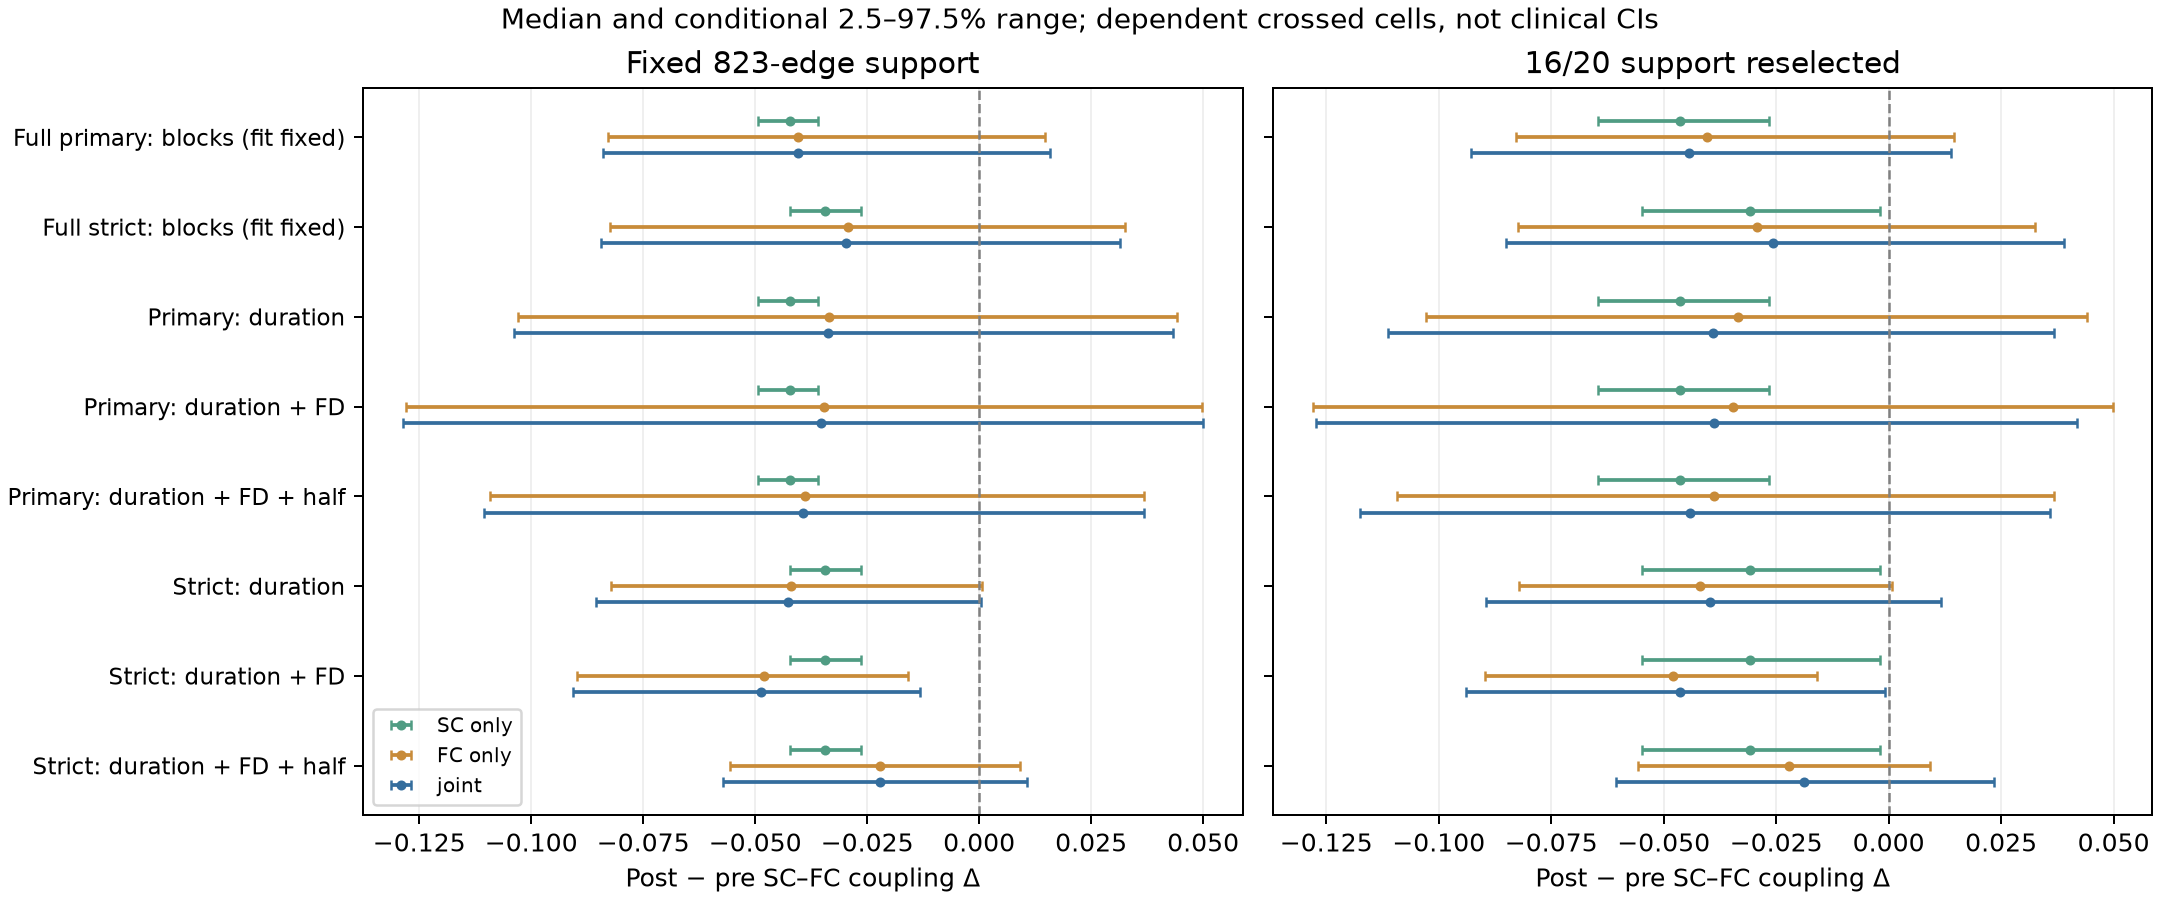
\includegraphics[width=\linewidth]{joint_sampling_ranges.png}
\caption{SC-only, FC-only and joint conditional sampling ranges, with observed support fixed (left) or reselected by the same 16/20 rule (right). FC-only retains the observed SC/support in both panels. Joint cells preserve within-tractogram and within-FC edge dependence. Support reselection changes the ranked edge population.}\label{fig:jointranges}\end{figure}

Reselecting consensus yields a median \JointSupportMedian{} common edges, with 2.5/97.5 percentiles \JointSupportLow{}/\JointSupportHigh{}; the median Jaccard overlap with the observed 823 edges is \JointJaccardMedian{}. The median numbers of added and removed edges are 36 and 33. The SC-only primary range widens to $[-0.06466,-0.02662]$, whereas full-primary joint sampling gives $\JointPrimaryReselectMedian{}$ $[\JointPrimaryReselectLow{},\JointPrimaryReselectHigh{}]$. The SC-only median shifts because a discontinuous support rule changes rank context. Reselected strict duration+FD gives $\JointStrictMotionReselectMedian{}$ $[\JointStrictMotionReselectLow{},\JointStrictMotionReselectHigh{}]$; its small negative upper endpoint and \JointStrictMotionReselectPositive{}\% positive fraction should not be described as a stable directional conclusion. Adding run-half matching gives $\JointStrictHalfReselectMedian{}$ $[\JointStrictHalfReselectLow{},\JointStrictHalfReselectHigh{}]$ (Table~\ref{tab:jointreselected}).
\begin{table}[H]\centering\scriptsize\setlength{\tabcolsep}{3pt}\begin{tabular}{lrrrrr}
\toprule
FC design & Median $\Delta$ & Conditional 95\% range & $\Delta>0$ (\%) & SC (\%) & FC (\%) \\
\midrule
Full primary, block 10 & -0.0444 & [-0.0929, +0.0138] & 6.84 & 10.8 & 84.2 \\
Full strict, block 10 & -0.0257 & [-0.0851, +0.0390] & 21.61 & 15.2 & 79.9 \\
Primary: duration & -0.0391 & [-0.1114, +0.0368] & 17.14 & 3.4 & 90.2 \\
Primary: duration + FD & -0.0388 & [-0.1273, +0.0418] & 15.51 & 3.1 & 91.1 \\
Primary: duration + FD + half & -0.0443 & [-0.1174, +0.0358] & 16.13 & 3.7 & 90.0 \\
Strict: duration & -0.0397 & [-0.0895, +0.0115] & 6.32 & 24.6 & 70.2 \\
Strict: duration + FD & -0.0464 & [-0.0939, -0.0009] & 2.29 & 31.8 & 62.6 \\
Strict: duration + FD + half & -0.0189 & [-0.0605, +0.0235] & 19.23 & 37.4 & 57.2 \\
\bottomrule
\end{tabular}

\caption{Selection sensitivity: reapply the same 16/20 rule in each bootstrapped session and rerank on its intersection. Unlike fixed-support inference, this includes a changing edge population. No outcome-based threshold tuning is performed.}\label{tab:jointreselected}\end{table}
\begin{figure}[H]\centering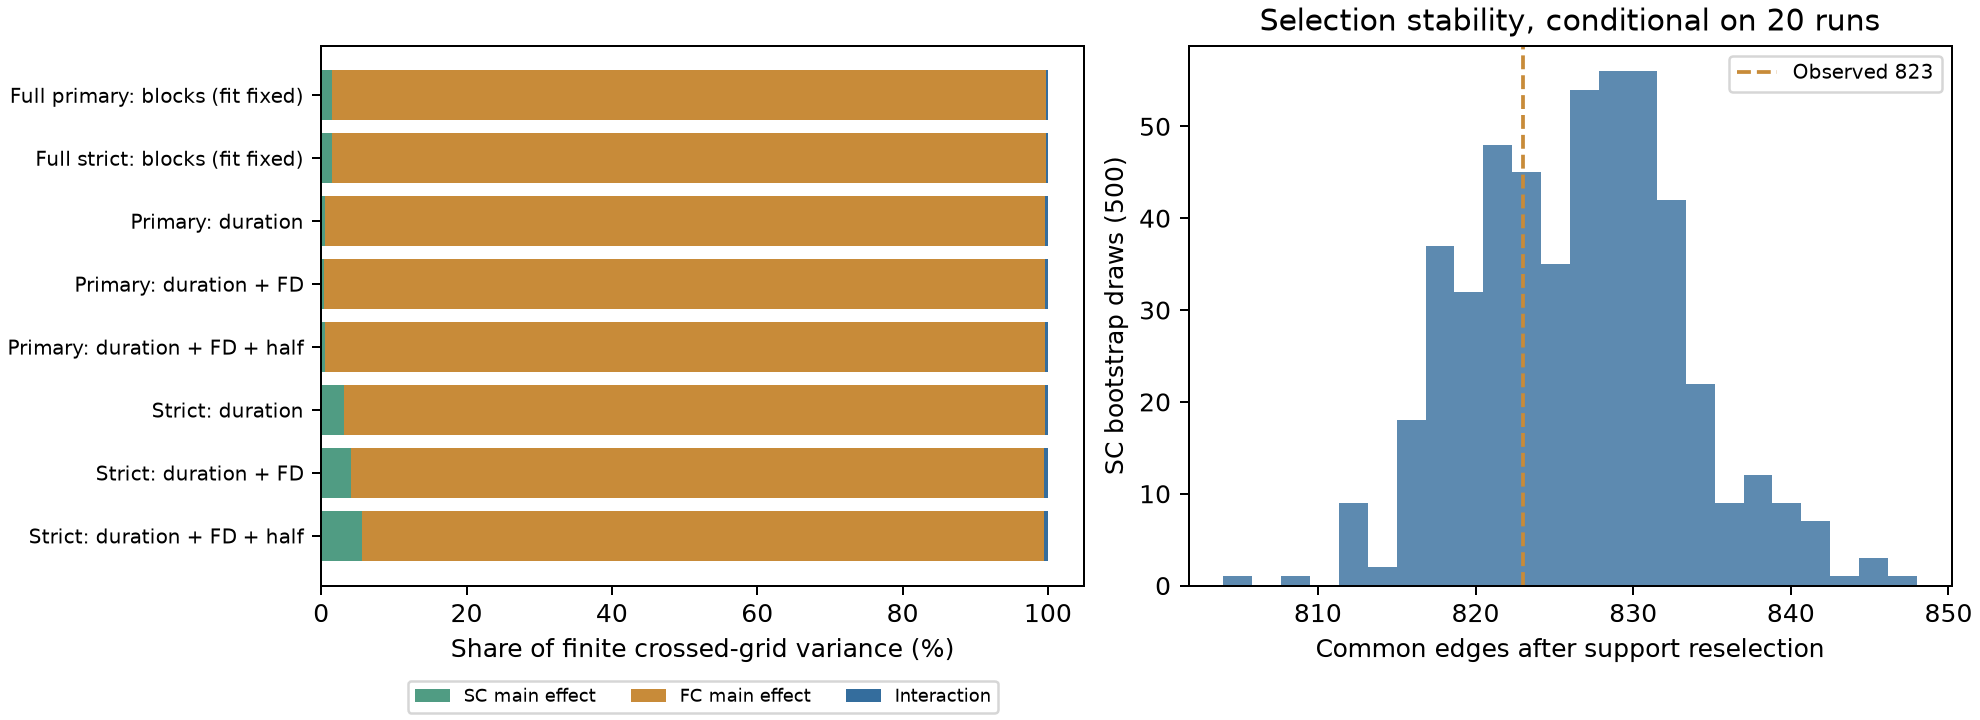
\includegraphics[width=\linewidth]{joint_sampling_components.png}
\caption{Fixed-support finite-grid variance shares (left) and selected common-support size across the 500 SC bootstrap draws (right). These are computational sensitivities under fixed imaging/model choices, not a partition of total clinical uncertainty.}\label{fig:jointcomponents}\end{figure}

Twelve- and forty-eight-second block sensitivities also yield zero-crossing full-primary/strict joint ranges in both support modes (Table~\ref{tab:jointblocks}). Matched draws retain rank 39 and residual df 29, while the original frozen block draws have no newly fitted nuisance rank/df. All 1,200 fixed-SC matched contrasts reproduce the preceding primary analysis to numerical precision. For reselected strict FD matching, splitting the FC ensemble into two halves moves the upper endpoint between $\JointTailHalfMin{}$ and $\JointTailHalfMax{}$: even its tail sign is sensitive to finite Monte Carlo sampling. Notebook 10 exports these half-ensemble checks, distinct-frame counts, every crossed cell and per-edge selection frequencies. The support/seed and temporal controls quantify specific conditional uncertainties together; they leave nuisance-model, acquisition and biological interpretations unresolved.
\begin{table}[H]\centering\small\begin{tabular}{lrlrr}
\toprule
Censor pool & Block frames & Support & Median $\Delta$ & Conditional 95\% range \\
\midrule
Primary & 5 & fixed & -0.0420 & [-0.0792, +0.0096] \\
Primary & 5 & reselected & -0.0453 & [-0.0870, +0.0074] \\
Primary & 10 & fixed & -0.0405 & [-0.0839, +0.0158] \\
Primary & 10 & reselected & -0.0444 & [-0.0929, +0.0138] \\
Primary & 20 & fixed & -0.0404 & [-0.0833, +0.0106] \\
Primary & 20 & reselected & -0.0433 & [-0.0908, +0.0079] \\
Strict & 5 & fixed & -0.0321 & [-0.0868, +0.0233] \\
Strict & 5 & reselected & -0.0266 & [-0.0891, +0.0313] \\
Strict & 10 & fixed & -0.0298 & [-0.0844, +0.0315] \\
Strict & 10 & reselected & -0.0257 & [-0.0851, +0.0390] \\
Strict & 20 & fixed & -0.0341 & [-0.0930, +0.0303] \\
Strict & 20 & reselected & -0.0288 & [-0.0951, +0.0422] \\
\bottomrule
\end{tabular}

\caption{Block-length sensitivity of joint temporal/seed sampling at full retained exposure. Nuisance fits are frozen. Block sizes are 5/10/20 original frames (12/24/48 s), selected as fixed sensitivity settings.}\label{tab:jointblocks}\end{table}

\subsection{Sensitivity: full-run bootstrap refits versus frozen training}\label{sec:refitresults}
All 200 primary paired draws pass the explicit safeguards at every block length. The ten-frame draws contain median 93.5/96 distinct pre/post frames, with minimum distinct rows minus rank 34/35. Strict sampling yields no eligible pre/post pair: pre-op eligibility is 0/200, 0/200 and 2/200 for blocks 5/10/20, while post-op eligibility is 129/200, 126/200 and 135/200 (Table~\ref{tab:refitfeasibility}). The two eligible strict pre-op block-20 draws do not coincide with eligible post-op draws. We therefore withhold strict full-run refit ranges. This is limited estimator feasibility under the explicit distinct-frame guard, not a statistical test of direction or evidence against conventional bootstrapping. Original all-draw frozen strict ranges and fully refitted 68-distinct-frame matched sensitivities remain available.
\begin{table}[H]\centering\small\begin{tabular}{llrrrr}
\toprule
Pool & Block & Pre eligible & Post eligible & Paired eligible & Median distinct pre/post \\
\midrule
Primary & 5 & 200/200 & 200/200 & 200/200 & 93/96 \\
Primary & 10 & 200/200 & 200/200 & 200/200 & 93.5/96 \\
Primary & 20 & 200/200 & 200/200 & 200/200 & 96/99 \\
Strict & 5 & 0/200 & 129/200 & 0/200 & 44/62 \\
Strict & 10 & 0/200 & 126/200 & 0/200 & 44.5/61 \\
Strict & 20 & 2/200 & 135/200 & 0/200 & 45/63 \\
\bottomrule
\end{tabular}

\caption{Requested full-run refits: eligibility requires 60 distinct frames, 15 distinct residual directions and numerical rank agreement. Paired eligibility requires both refitting conditions in both sessions. Attempted exposure remains 146/150 primary and 68/96 strict frames including repeats.}\label{tab:refitfeasibility}\end{table}

At fixed primary support with ten-frame blocks, frozen joint $\Delta$ has median $\RefitFrozenMedian{}$ and central range $[\RefitFrozenLow{},\RefitFrozenHigh{}]$. Refitting coefficients alone gives $\RefitCoefficientsMedian{}$ $[\RefitCoefficientsLow{},\RefitCoefficientsHigh{}]$. Full PC/regression refitting gives $\RefitFullMedian{}$ $[\RefitFullLow{},\RefitFullHigh{}]$ (Table~\ref{tab:refit}). The full range is wider and its center closer to zero; \RefitFullPositive{}\% of dependent grid cells are positive versus \RefitFrozenPositive{}\% frozen. These fractions are computational sensitivity summaries, not posterior probabilities of improvement. FC accounts for \RefitFullFCShare{}\% of the finite crossed-grid variance in the full-refit experiment. No negative biological direction is established.
\begin{table}[H]\centering\scriptsize\setlength{\tabcolsep}{3pt}\begin{tabular}{llrrrr}
\toprule
Support & Nuisance training & Median $\Delta$ & Conditional 95\% range & $\Delta>0$ (\%) & FC (\%) \\
\midrule
fixed & Frozen & -0.0405 & [-0.0839, +0.0158] & 9.2 & 98.2 \\
fixed & Refit coefficients & -0.0436 & [-0.0980, +0.0364] & 11.8 & 99.0 \\
fixed & Refit PCs + coefficients & -0.0207 & [-0.0919, +0.0544] & 32.1 & 99.1 \\
reselected & Frozen & -0.0444 & [-0.0929, +0.0138] & 6.8 & 84.2 \\
reselected & Refit coefficients & -0.0470 & [-0.1056, +0.0337] & 9.8 & 89.3 \\
reselected & Refit PCs + coefficients & -0.0287 & [-0.0980, +0.0513] & 25.8 & 90.7 \\
\bottomrule
\end{tabular}

\caption{Primary ten-frame blocks: same 200 paired FC draws crossed with the same 500 SC bootstraps under three nuisance conditions. The observed point contrast remains $-0.04173$. Reselection changes the ranked connection population. FC column is its finite-grid variance share.}\label{tab:refit}\end{table}
\begin{figure}[H]\centering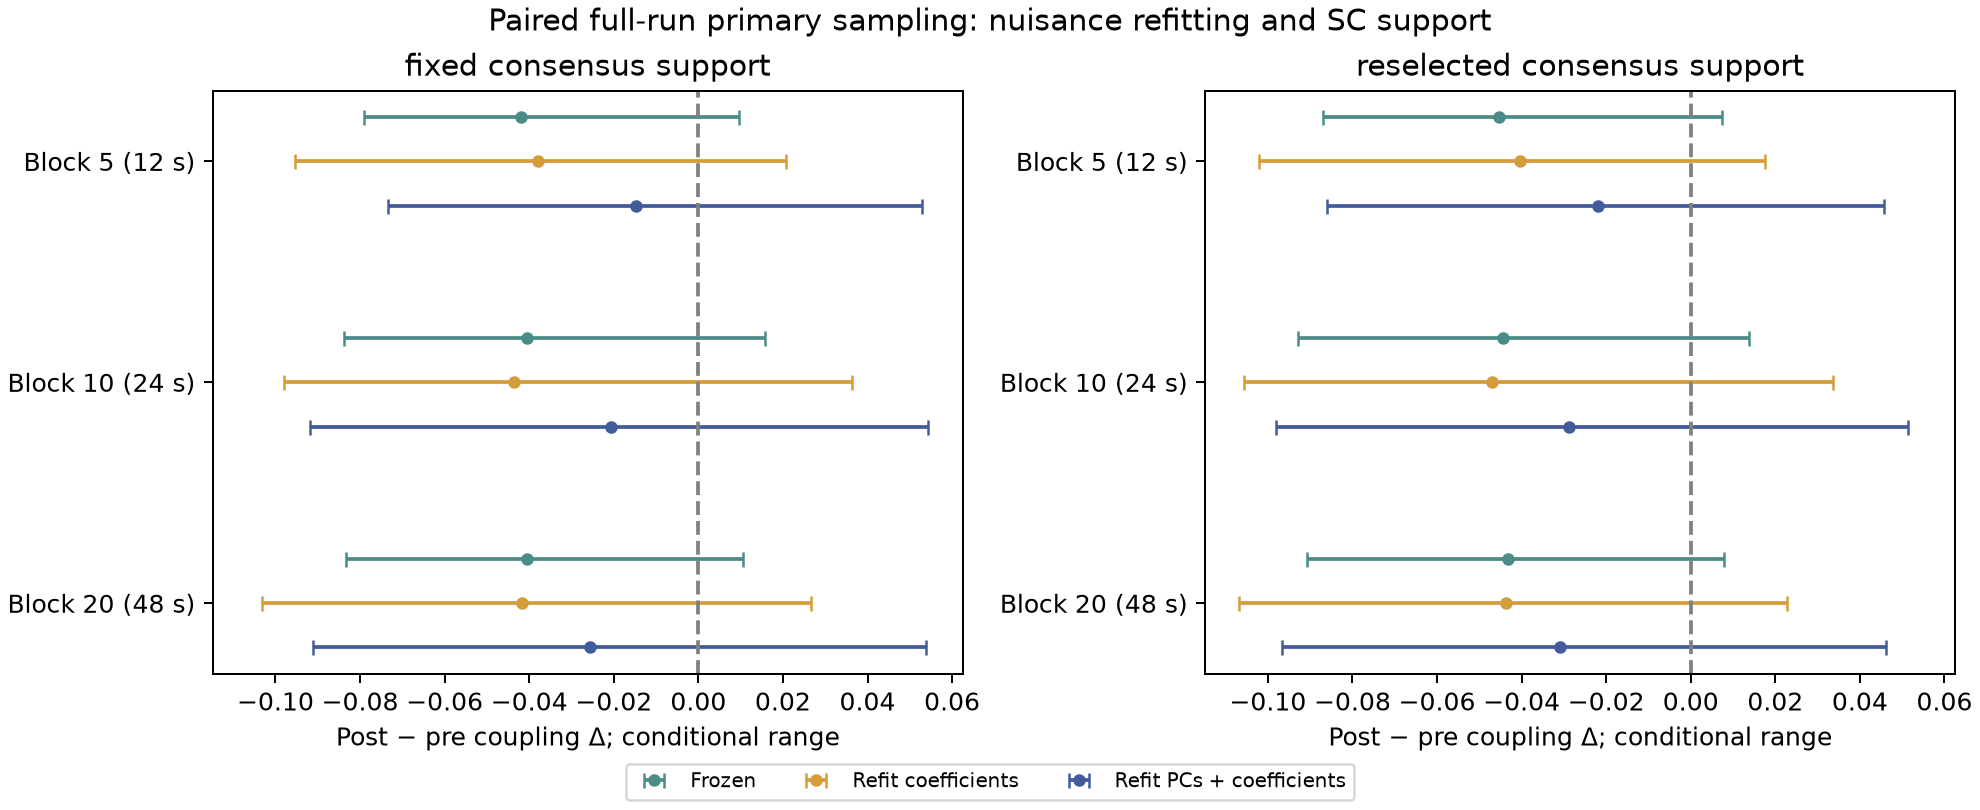
\includegraphics[width=\linewidth]{joint_refit_ranges.png}
\caption{Full-run primary sensitivity to regression/PC retraining and block length. Frozen and refitted models use exactly the same draws. These conditional ranges do not cover acquisition, spatial-mask, model-choice or clinical measurement uncertainty.}\label{fig:refit}\end{figure}

The paired shift full-minus-frozen has median $+0.01798$ and range $[-0.03827,+0.07335]$. Its ordered components are coefficient-minus-frozen and full-minus-coefficient (Table~\ref{tab:refitshifts}); they sum exactly for each cell, although their marginal medians need not sum. The further PC-training shift has median $+0.02350$, whereas the coefficient-only shift has median $-0.00265$. PC retraining is therefore consequential beyond coefficient refitting in this experiment; neither shift identifies neural signal removal or independent causal mechanisms. Median minimum squared cosines between the five-dimensional baseline/refitted PC spans are 0.0479 pre-op and 0.1147 post-op, after multiplicity weighting. Both sessions' nuisance subspaces can change substantially; this is not uniquely a postoperative phenomenon.
\begin{table}[H]\centering\small\begin{tabular}{lrr}
\toprule
Paired contrast shift & Median & Conditional 95\% range \\
\midrule
Coefficients minus frozen & -0.0026 & [-0.0424, +0.0430] \\
Full minus coefficients & +0.0235 & [-0.0310, +0.0725] \\
Full minus frozen & +0.0180 & [-0.0383, +0.0733] \\
\bottomrule
\end{tabular}

\caption{Paired shifts of the longitudinal contrast, fixed support and ten-frame blocks. Every subtraction uses the same SC bootstrap and FC draw, not differences between unpaired distributions.}\label{tab:refitshifts}\end{table}
\begin{table}[H]\centering\scriptsize\setlength{\tabcolsep}{4pt}\begin{tabular}{rllrr}
\toprule
Block & Support & Nuisance training & Median $\Delta$ & Conditional 95\% range \\
\midrule
5 & fixed & Frozen & -0.0420 & [-0.0792, +0.0096] \\
5 & fixed & Refit coefficients & -0.0379 & [-0.0953, +0.0208] \\
5 & fixed & Refit PCs + coefficients & -0.0147 & [-0.0733, +0.0528] \\
5 & reselected & Frozen & -0.0453 & [-0.0870, +0.0074] \\
5 & reselected & Refit coefficients & -0.0404 & [-0.1021, +0.0176] \\
5 & reselected & Refit PCs + coefficients & -0.0220 & [-0.0860, +0.0456] \\
10 & fixed & Frozen & -0.0405 & [-0.0839, +0.0158] \\
10 & fixed & Refit coefficients & -0.0436 & [-0.0980, +0.0364] \\
10 & fixed & Refit PCs + coefficients & -0.0207 & [-0.0919, +0.0544] \\
10 & reselected & Frozen & -0.0444 & [-0.0929, +0.0138] \\
10 & reselected & Refit coefficients & -0.0470 & [-0.1056, +0.0337] \\
10 & reselected & Refit PCs + coefficients & -0.0287 & [-0.0980, +0.0513] \\
20 & fixed & Frozen & -0.0404 & [-0.0833, +0.0106] \\
20 & fixed & Refit coefficients & -0.0418 & [-0.1032, +0.0266] \\
20 & fixed & Refit PCs + coefficients & -0.0256 & [-0.0912, +0.0538] \\
20 & reselected & Frozen & -0.0433 & [-0.0908, +0.0079] \\
20 & reselected & Refit coefficients & -0.0438 & [-0.1067, +0.0227] \\
20 & reselected & Refit PCs + coefficients & -0.0308 & [-0.0967, +0.0462] \\
\bottomrule
\end{tabular}

\caption{All primary block-length/support/model combinations. Each range uses 200 eligible paired FC draws and 500 SC draws. Centers and widths depend on both retraining and temporal scale; no setting is selected by its sign.}\label{tab:refitblocks}\end{table}

Full-refit fixed-support medians range from $-0.0147$ to $-0.0256$ across block lengths, with all central ranges crossing zero. Support-reselected ten-frame full refits give median $-0.02871$ and range $[-0.09801,+0.05130]$. As in the frozen study, support selection changes ranks and populations. Monte Carlo half-ensemble summaries are saved for all eligible conditions; they diagnose finite simulation variation rather than validate calibration. The observed point estimates are not replaced by bootstrap medians: retraining on repeated rows changes the empirical training distribution and can markedly displace empirical centers, especially for network FC averages. Section~\ref{sec:pcsamplingresults} diagnoses that displacement; population bias is not identified from these conditional experiments.

\subsection{Why PC refitting recenters the sampling distributions}\label{sec:pcsamplingresults}
All 200 paired draws pass the safeguards for each of the 12 primary designs, with rank 39 in each refit. Maximum FC difference from the preceding bootstrap replay is $1.82\times10^{-12}$. This excludes a changed baseline or replay implementation as the explanation. At ten-frame blocks, bootstrap median distinct counts are 93.5/96 pre/post, despite 146/150 rows; frequency Kish counts are 76.1/78.7. Unit coverage and matched-count blocks retain those exact distinct counts, while 80\% blocks retain 116/120 (Table~\ref{tab:pcsamplingqc}). None estimates independent effective sample size.
\begin{table}[H]\centering\small\begin{tabular}{llrrrr}
\toprule
Sampling & Session & Rows & Distinct & Kish count & Mean FD \\
\midrule
Bootstrap & preop & 146 & 93.5 & 76.1 & 0.289 \\
Bootstrap & postop & 150 & 96 & 78.7 & 0.251 \\
Same frames, unit weights & preop & 93.5 & 93.5 & 93.5 & 0.289 \\
Same frames, unit weights & postop & 96 & 96 & 96.0 & 0.252 \\
Blocks, matched count & preop & 93.5 & 93.5 & 93.5 & 0.287 \\
Blocks, matched count & postop & 96 & 96 & 96.0 & 0.251 \\
Blocks, 80\% retained & preop & 116 & 116 & 116.0 & 0.287 \\
Blocks, 80\% retained & postop & 120 & 120 & 120.0 & 0.253 \\
\bottomrule
\end{tabular}

\caption{Ten-frame designs: median per-session draw QC. FD is mm; Kish count describes frequency-weight concentration. Matched distinct count does not equate FD or temporal coverage. All 200 paired draws are eligible in every design.}\label{tab:pcsamplingqc}\end{table}

\textbf{Loading retraining dominates the paired shift.} Temporal-only refitting changes FC by at most $3.20\times10^{-13}$ and leaves coupling identical, as predicted by the shared temporal span. Preprocessing-only minus fixed-PC contrast shifts have median $+0.00005$ and range $[-0.00179,+0.00164]$. With preprocessing frozen, loading refits instead give a median shift $+0.02059$ $[-0.03147,+0.06871]$, compared with $+0.02350$ $[-0.03103,+0.07246]$ for full refits (Tables~\ref{tab:pcmechanism}--\ref{tab:pcshifts}). Subsequent preprocessing after loading refits adds median $+0.00141$, with substantial draw variation; increments and their medians are order dependent. This computational intervention implicates the learned PCA space, not PC sign flips or temporal projection alone.
\begin{table}[H]\centering\small\begin{tabular}{lrr}
\toprule
Training intervention & Median $\Delta$ & Conditional range \\
\midrule
Frozen PCs; refit regression & -0.04364 & [-0.09795, +0.03636] \\
Temporal projection only & -0.04364 & [-0.09795, +0.03636] \\
Preprocessing only & -0.04366 & [-0.09791, +0.03619] \\
PCA loadings only & -0.02275 & [-0.09957, +0.05616] \\
Preprocessing + loadings & -0.02069 & [-0.09189, +0.05442] \\
\bottomrule
\end{tabular}

\caption{Same ten-frame frequency-weighted draws and SC bootstraps, with regression refitted in every condition. ``Preprocessing'' includes tissue temporal projection and voxel scaling; ``loadings'' means the spatial five-PC basis.}\label{tab:pcmechanism}\end{table}
\begin{table}[H]\centering\small\begin{tabular}{lrr}
\toprule
Paired shift in longitudinal contrast & Median & Conditional range \\
\midrule
Temporal only minus frozen PCs & +0.00000 & [+0.00000, +0.00000] \\
Preprocessing only minus frozen PCs & +0.00005 & [-0.00179, +0.00164] \\
Full minus preprocessing only & +0.02332 & [-0.03191, +0.07305] \\
Loadings only minus frozen PCs & +0.02059 & [-0.03147, +0.06871] \\
Full minus loadings only & +0.00141 & [-0.01830, +0.02254] \\
Full minus frozen PCs & +0.02350 & [-0.03103, +0.07246] \\
\bottomrule
\end{tabular}

\caption{Exactly paired shifts of the post-minus-pre coupling contrast. Conditional ranges summarize dependent crossed cells. Marginal medians do not form an additive decomposition.}\label{tab:pcshifts}\end{table}
\begin{figure}[H]\centering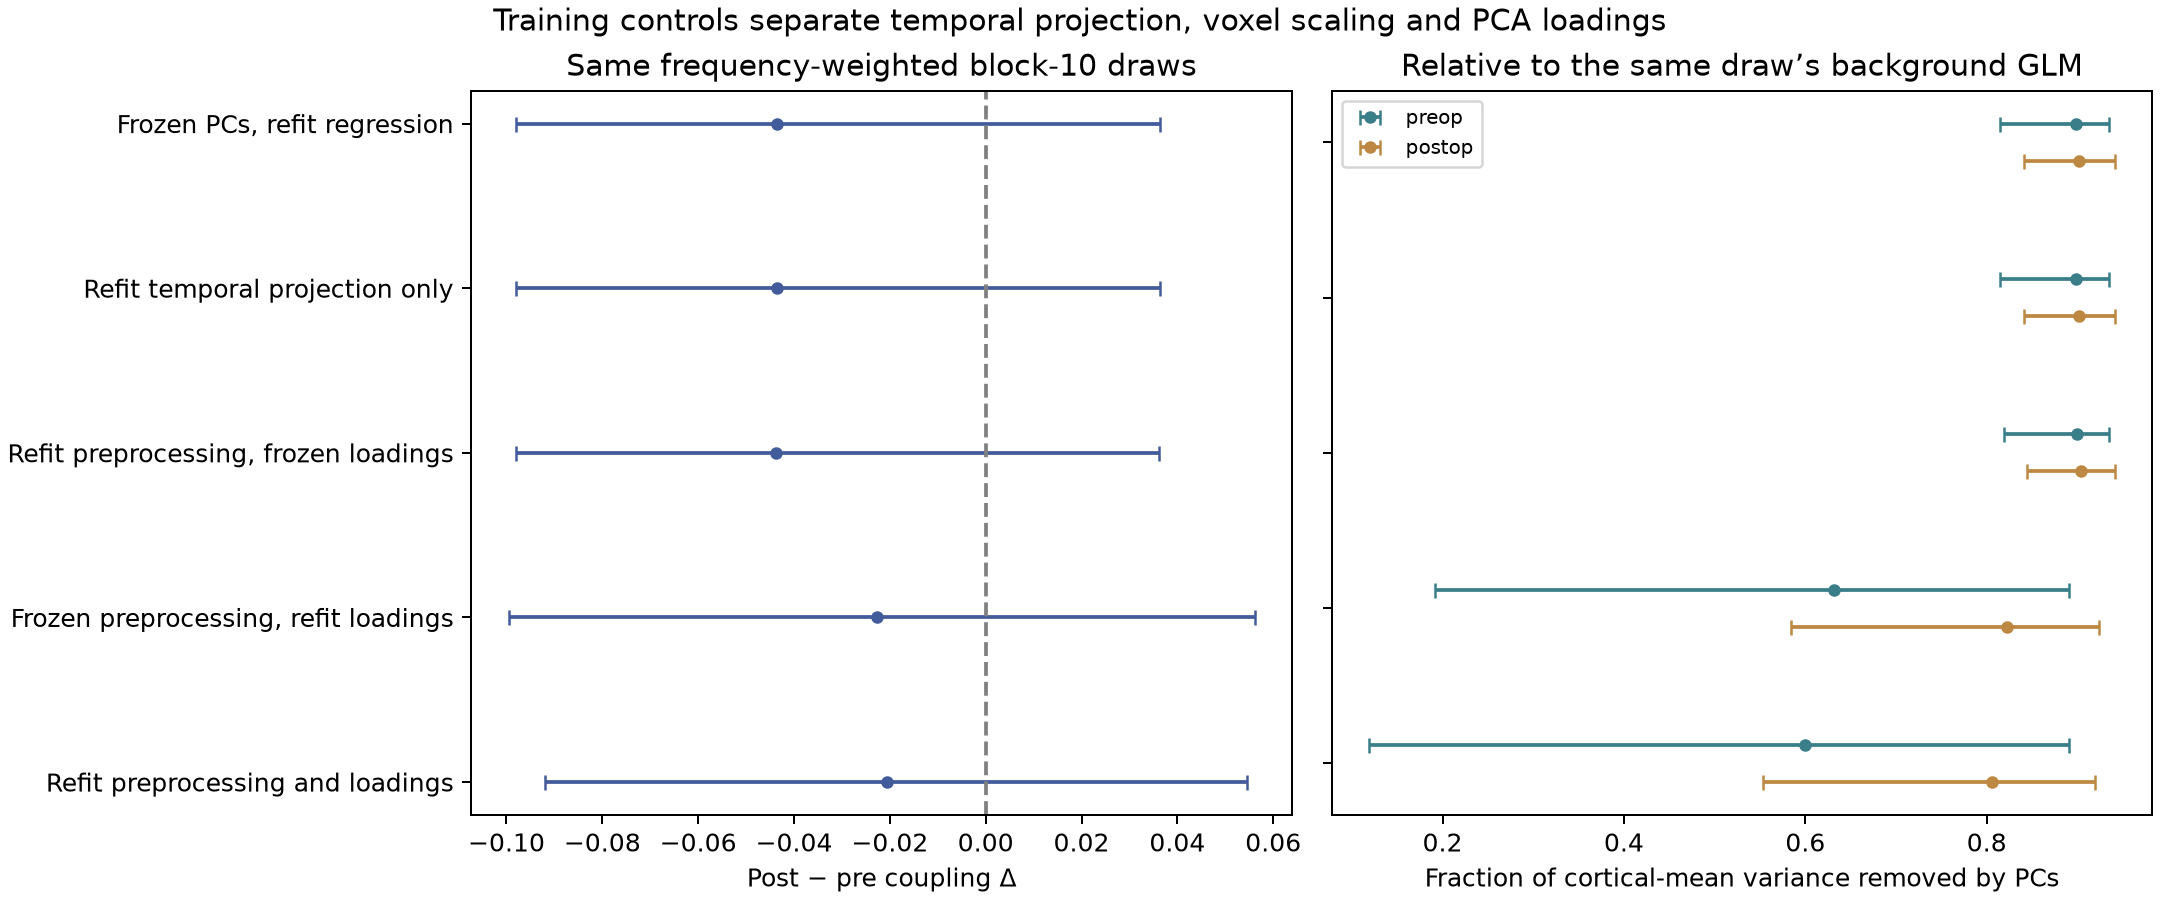
\includegraphics[width=\linewidth]{pc_sampling_mechanism.png}
\caption{Training interventions change the ranked coupling contrast and the amount of shared cortical-mean signal removed by PCs. Removal is relative to the same draw's background GLM; its neural/nuisance composition is unknown.}\label{fig:pcsamplingmechanism}\end{figure}

\textbf{Repeated-frame weighting changes which tissue directions enter the five-PC model.} After common-background projection, median minimum PC-span cosine squared is 0.033 pre-op and 0.082 post-op for full bootstrap refits, versus 0.278/0.618 at unit coverage, 0.234/0.635 for independently sampled matched-count blocks and 0.391/0.820 at 80\% retention (Table~\ref{tab:pcstability}). Thus the discrepancy persists after removing already-modelled motion/trend/DCT directions, and both sessions are affected. Baseline relative eigenvalue gaps at the fifth/sixth boundary are 0.015/0.046; these are compatible with a sensitive truncated space, without demonstrating a single PC swap. Bootstrap median gaps become 0.056/0.052 even while spans change substantially. A large within-draw gap therefore does not certify agreement with baseline.

Five PCs capture median 19.2\%/21.0\% of tissue variance after bootstrap retraining versus baseline 15.1\%/17.4\%, yet remove less cortical-mean signal. With PCs frozen and coefficients refitted, median cortical-mean variance removed is 89.9\%/90.2\%; full bootstrap refits remove 60.0\%/80.6\%. Median mean FC rises from 0.079/0.047 to 0.231/0.087, especially pre-op. PCA optimizes the weighted tissue covariance, not removal of any particular cortical signal. Unit coverage restores median removal to 84.9\%/88.7\%, and 80\% retention to 89.7\%/89.5\%. This links weighting, altered nuisance subspaces and changed residual shared-signal content computationally, without identifying that signal's origin.
\begin{table}[H]\centering\scriptsize\setlength{\tabcolsep}{3pt}\begin{tabular}{llrrrrr}
\toprule
Sampling & Session & Min $\cos^2$ & Gap$_{5/6}$ & PC var. (\%) & Mean removed (\%) & FC $r$ \\
\midrule
Bootstrap & preop & 0.033 & 0.056 & 19.2 & 60.0 & 0.231 \\
Bootstrap & postop & 0.082 & 0.052 & 21.0 & 80.6 & 0.087 \\
Same frames, unit weights & preop & 0.278 & 0.048 & 17.1 & 84.9 & 0.118 \\
Same frames, unit weights & postop & 0.618 & 0.051 & 19.3 & 88.7 & 0.054 \\
Blocks, matched count & preop & 0.234 & 0.048 & 17.2 & 85.0 & 0.111 \\
Blocks, matched count & postop & 0.635 & 0.051 & 19.4 & 88.8 & 0.054 \\
Blocks, 80\% retained & preop & 0.391 & 0.040 & 16.0 & 89.7 & 0.090 \\
Blocks, 80\% retained & postop & 0.820 & 0.051 & 18.3 & 89.5 & 0.050 \\
\bottomrule
\end{tabular}

\caption{Median diagnostics for full refits, ten-frame designs. Minimum squared cosine is conditional on the common background. Gap is relative eigenvalue separation at 5/6; PC variance is the tissue fraction captured. ``Mean removed'' is cortical-mean variance removed relative to the same draw's background GLM. FC is mean pairwise correlation.}\label{tab:pcstability}\end{table}
\begin{figure}[H]\centering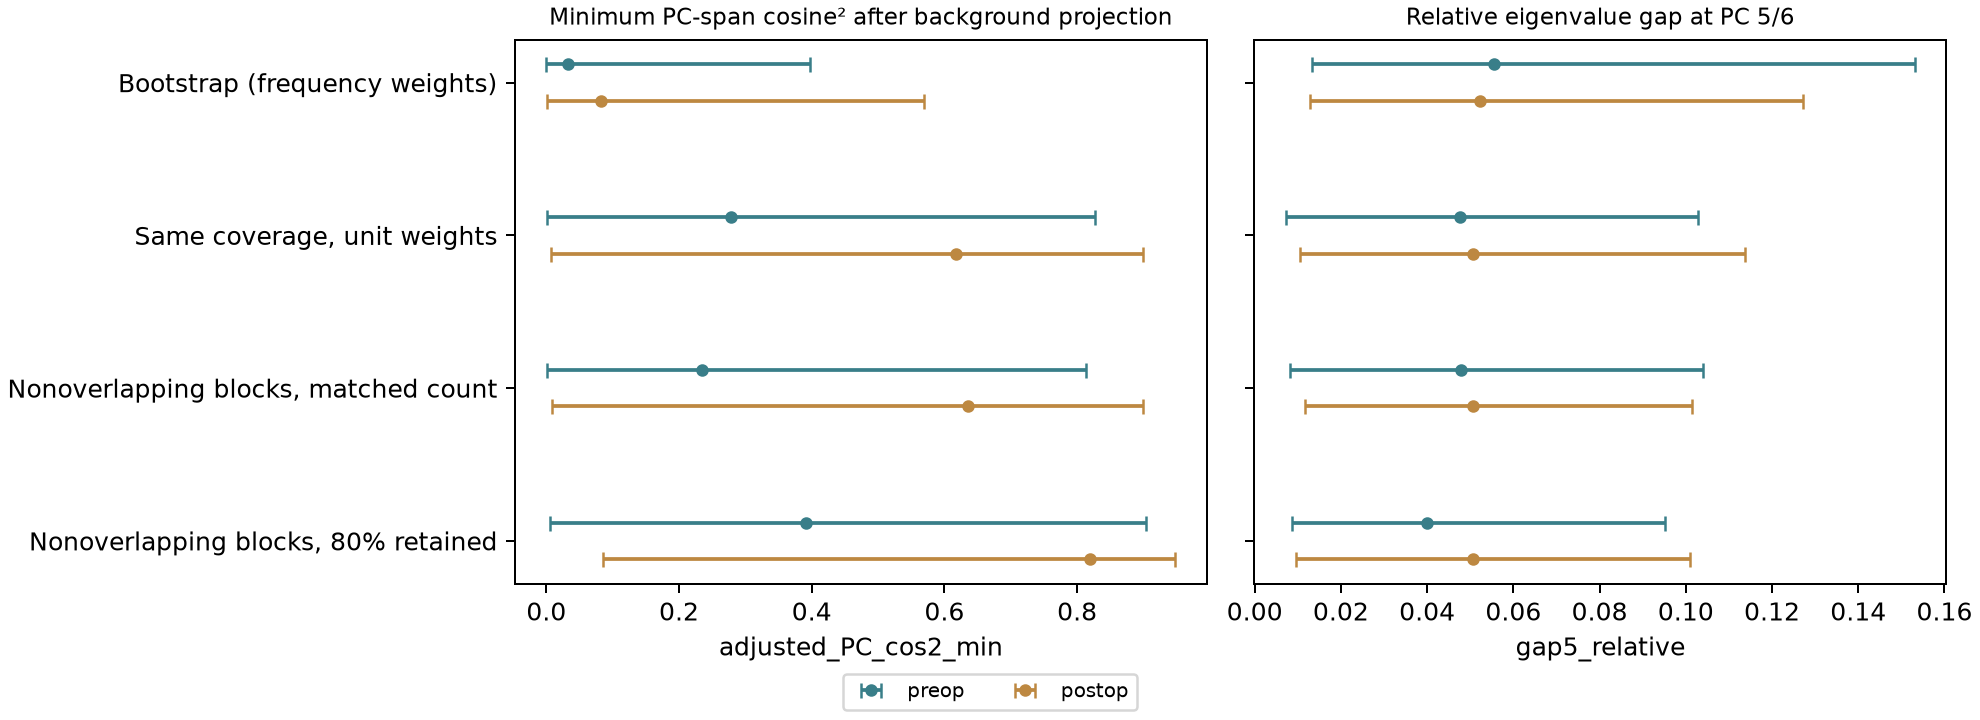
\includegraphics[width=\linewidth]{pc_sampling_stability.png}
\caption{PC overlap and boundary separation across sampling designs, median and central 2.5/97.5 percentiles. The two diagnostics answer different questions; neither validates physiological specificity.}\label{fig:pcstability}\end{figure}

\textbf{Multiplicity removal largely removes the global recentering.} With fixed SC support, ten-frame full-refit median $\Delta$ is $-0.02069$ $[-0.09189,+0.05442]$ under the bootstrap, $-0.04366$ $[-0.09162,+0.02834]$ at unit coverage, and $-0.04001$ $[-0.10186,+0.02461]$ with independent matched-count blocks (Table~\ref{tab:pcsampling}). In the latter two, coefficient-only centers are $-0.04418$ and $-0.03997$: the further loading/preprocessing recentering is small. Full-bootstrap pre-op coupling median falls from 0.1731 to 0.1447 after PC refits, while post-op falls from 0.1289 to 0.1231, moving the longitudinal contrast toward zero. At unit coverage these are 0.1759 to 0.1736 and 0.1316 to 0.1303. Session medians do not algebraically determine the median paired contrast. The paired full-minus-coefficient shift falls from median $+0.02350$ in the bootstrap to $+0.00033$ at unit coverage and $-0.00128$ with matched-count blocks. These comparisons separate repeated-frame weights from reduced distinct coverage; no single contributor is asserted to explain every network statistic.
\begin{table}[H]\centering\footnotesize\begin{tabular}{llrr}
\toprule
Sampling & Nuisance fit & Median $\Delta$ & Conditional range \\
\midrule
Bootstrap & Frozen & -0.0405 & [-0.0839, +0.0158] \\
Bootstrap & Refit coefficients & -0.0436 & [-0.0980, +0.0364] \\
Bootstrap & Refit PCs + coefficients & -0.0207 & [-0.0919, +0.0544] \\
Same frames, unit weights & Frozen & -0.0401 & [-0.0759, +0.0048] \\
Same frames, unit weights & Refit coefficients & -0.0442 & [-0.0931, +0.0296] \\
Same frames, unit weights & Refit PCs + coefficients & -0.0437 & [-0.0916, +0.0283] \\
Blocks, matched count & Frozen & -0.0386 & [-0.0771, +0.0018] \\
Blocks, matched count & Refit coefficients & -0.0400 & [-0.0955, +0.0224] \\
Blocks, matched count & Refit PCs + coefficients & -0.0400 & [-0.1019, +0.0246] \\
Blocks, 80\% retained & Frozen & -0.0415 & [-0.0674, -0.0173] \\
Blocks, 80\% retained & Refit coefficients & -0.0434 & [-0.0835, -0.0078] \\
Blocks, 80\% retained & Refit PCs + coefficients & -0.0478 & [-0.0915, -0.0114] \\
\bottomrule
\end{tabular}

\caption{Ten-frame sampling comparison, fixed primary SC support, 500 SC by 200 FC dependent cells per range. Point $\Delta=-0.04173$ is unchanged. Unit coverage is a paired multiplicity control; the other new designs sample blocks without replacement.}\label{tab:pcsampling}\end{table}
\begin{figure}[H]\centering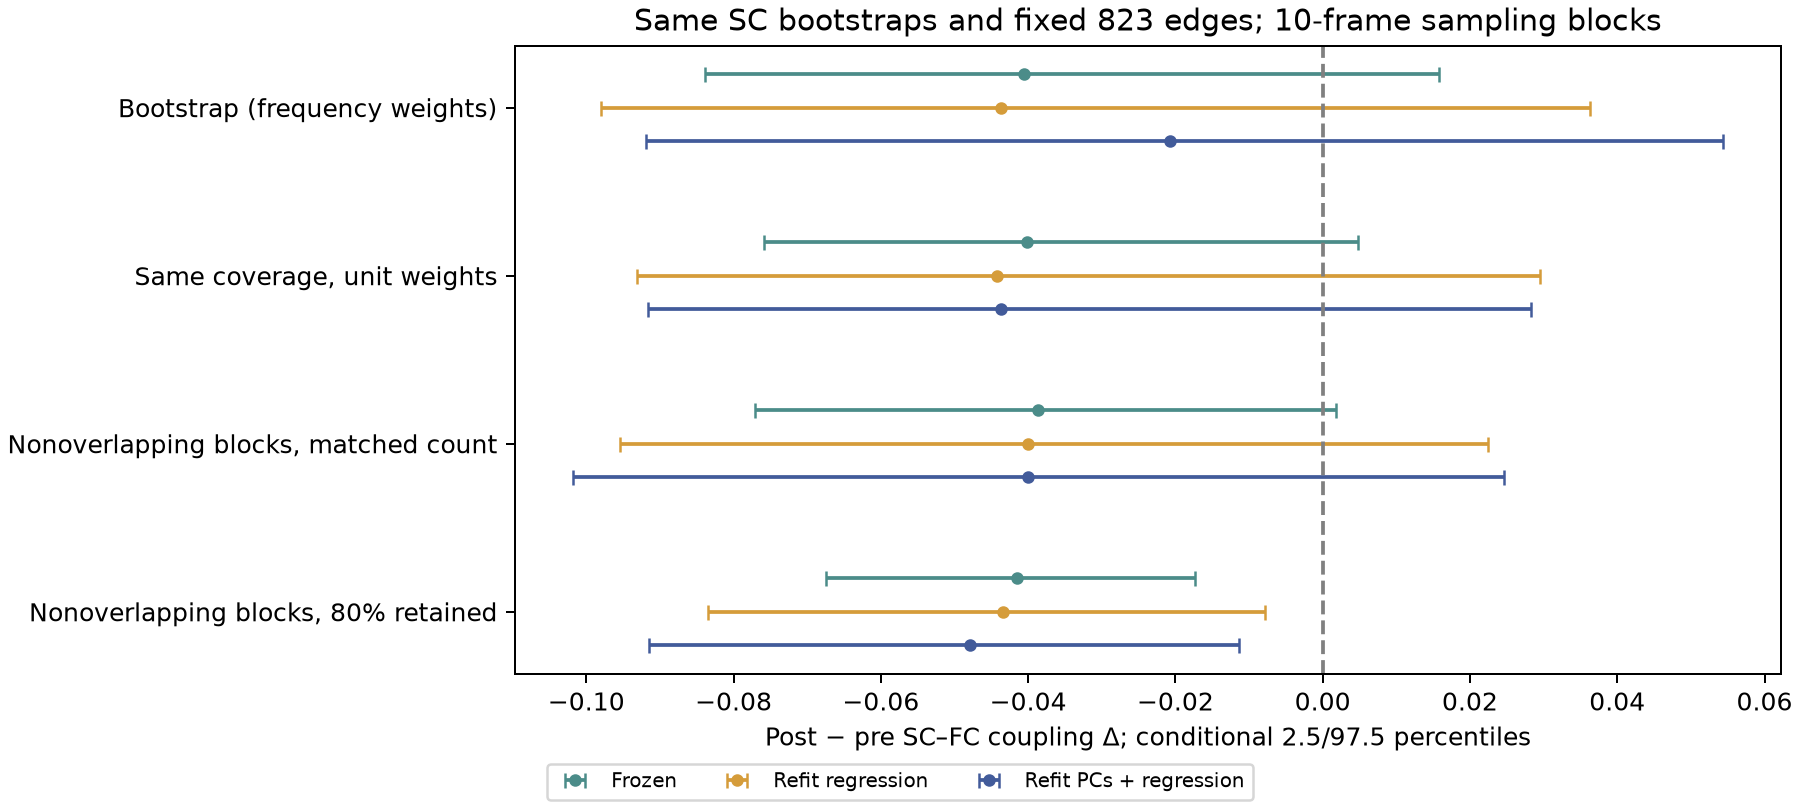
\includegraphics[width=\linewidth]{pc_sampling_ranges.png}
\caption{Full versus frozen training across four designs. The 80\% subset range pertains to a larger retained fraction than the matched-count subsets, not an interchangeable full-run confidence interval.}\label{fig:pcsampling}\end{figure}

At 80\% retention, the full-refit median is $-0.04784$ $[-0.09155,-0.01139]$. Full-refit medians for independent matched-count blocks vary only from $-0.03912$ to $-0.04017$ across block lengths; their ranges all span zero. The 80\% ranges remain negative across these lengths (Table~\ref{tab:pcblocks}), but their fraction-dependent shrinkage cannot establish a biological sign. At 100\% the tested sampler/refit identity recovers observed FC with zero FC sampling variance. Reselected-support ten-frame full-refit ranges are $[-0.10129,+0.02695]$ at unit coverage, $[-0.10946,+0.02373]$ for matched-count blocks and $[-0.09544,-0.01133]$ at 80\%. Support sensitivity does not settle calibration. We retain complete refitting for the estimator's sampling analysis and present both bootstrap and nonreplacement controls; none is selected by its sign, bias-corrected, or elevated to a calibrated population interval. Notebook 13 exposes all draws, contrasts and QC; \path{results/pc_sampling} stores their lineage and outputs.
\begin{table}[H]\centering\small\begin{tabular}{rlrr}
\toprule
Block & Sampling & Median $\Delta$ & Conditional range \\
\midrule
5 & Bootstrap & -0.0147 & [-0.0733, +0.0528] \\
5 & Same frames, unit weights & -0.0375 & [-0.0905, +0.0257] \\
5 & Blocks, matched count & -0.0402 & [-0.1002, +0.0206] \\
5 & Blocks, 80\% retained & -0.0443 & [-0.0858, -0.0060] \\
10 & Bootstrap & -0.0207 & [-0.0919, +0.0544] \\
10 & Same frames, unit weights & -0.0437 & [-0.0916, +0.0283] \\
10 & Blocks, matched count & -0.0400 & [-0.1019, +0.0246] \\
10 & Blocks, 80\% retained & -0.0478 & [-0.0915, -0.0114] \\
20 & Bootstrap & -0.0256 & [-0.0912, +0.0538] \\
20 & Same frames, unit weights & -0.0395 & [-0.1013, +0.0304] \\
20 & Blocks, matched count & -0.0391 & [-0.1071, +0.0228] \\
20 & Blocks, 80\% retained & -0.0431 & [-0.0822, -0.0026] \\
\bottomrule
\end{tabular}

\caption{Full-refit block-length sensitivity at fixed SC support. Ranges are conditional on design, retained fraction and fixed preprocessing assets. All cells reuse the same whole-run SC bootstrap ensemble.}\label{tab:pcblocks}\end{table}

\subsection{Historical sensitivity: why stricter censoring reversed coupling}\label{sec:censoringresults}
This subsection preserves the original seed-160 own-support investigation (1,515/1,559 edges). Its coupling figures/tables are historical sensitivities; the current common-consensus counterparts are in Section~\ref{sec:primaryscresults}. Strict censoring reduces retained-frame mean FD from 0.2869/0.2522 to 0.2170/0.2088 mm (pre/post), while leaving 68/96 frames. These FD summaries concern retained samples; Table~\ref{tab:qc} reports all frames after the initial four. Strict retained counts in acquisition thirds are 35/12/21 preoperatively and 39/34/23 postoperatively (Fig.~\ref{fig:censorframes}). Retained samples span 6.96/6.76 minutes but provide 2.72/3.84 minutes of exposure. Thus stricter censoring changes duration, temporal coverage and nuisance training together.

\begin{figure}[H]\centering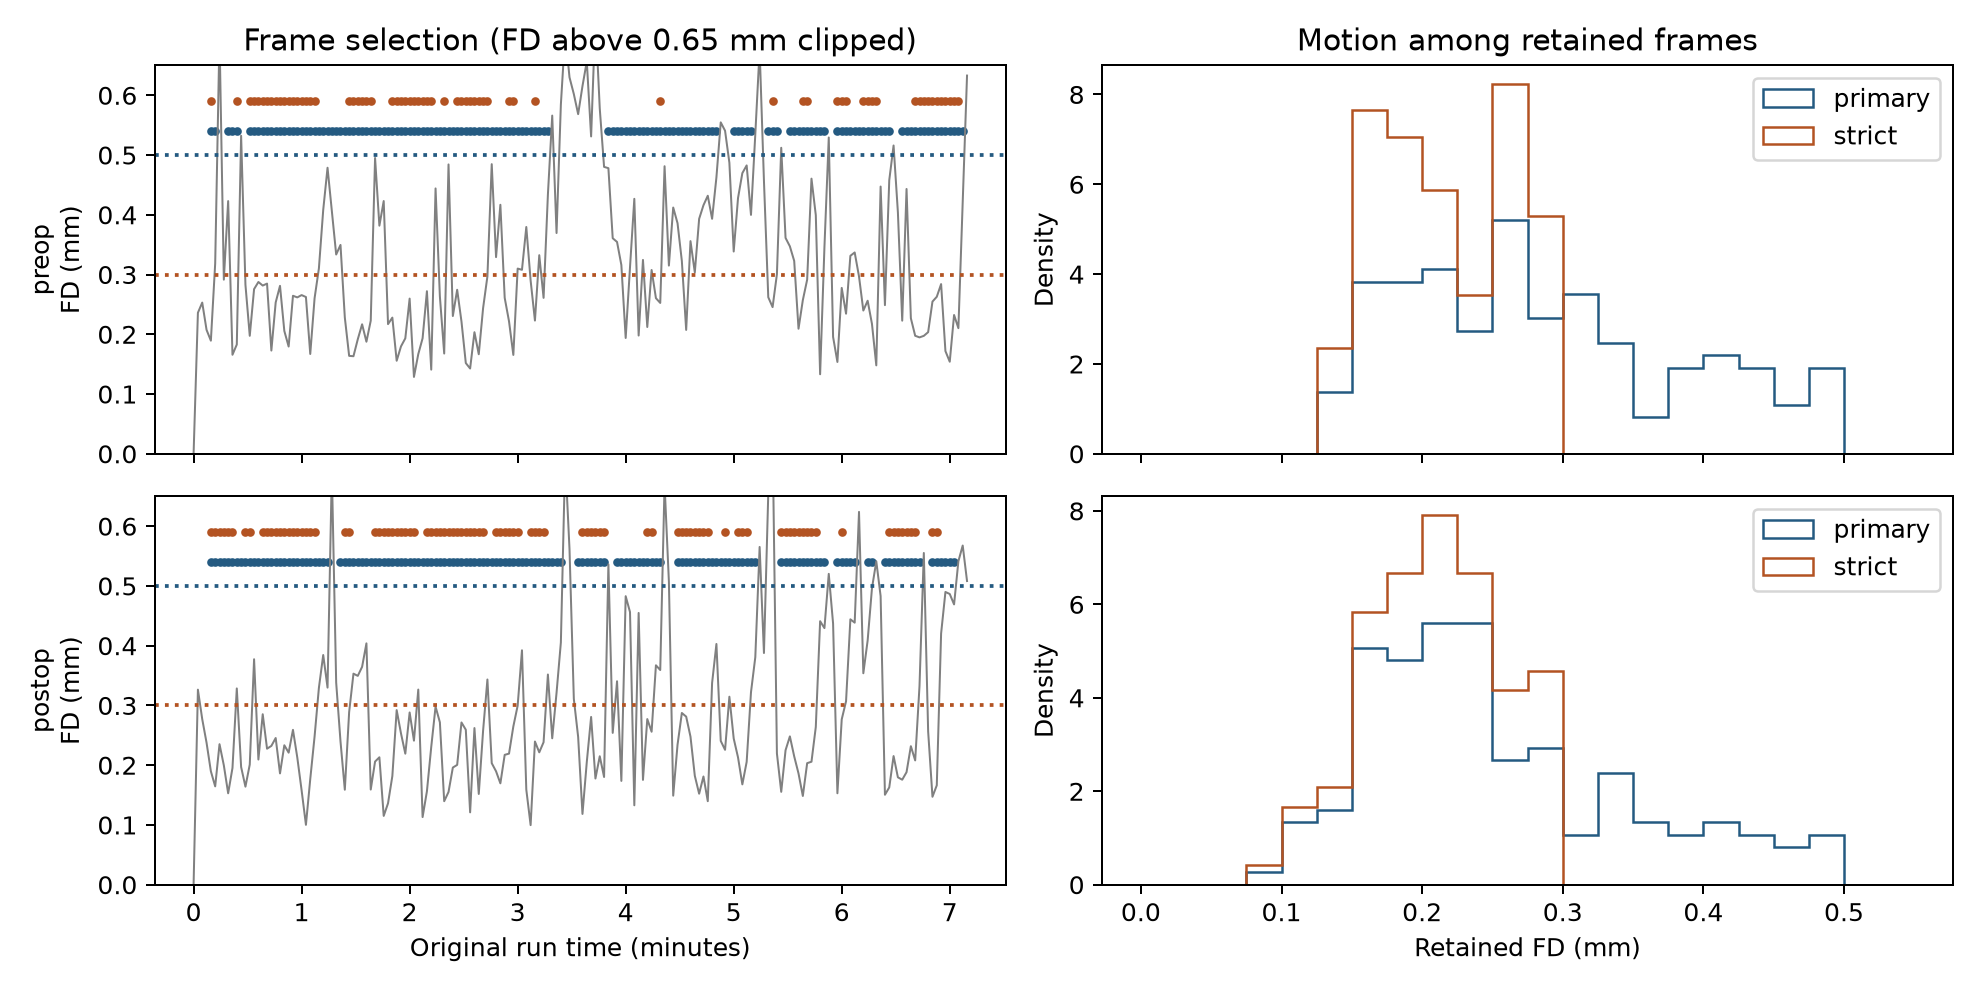
\includegraphics[width=\linewidth]{censoring_frame_qc.png}
\caption{Original-axis FD and retained samples, and retained-frame FD distributions. The FD trace is clipped above 0.65 mm for visibility; no high-FD samples enter the strict/primary pools. Orange strict samples occupy different parts of the runs, despite fairly similar retained-motion distributions.}\label{fig:censorframes}\end{figure}

The ordered decomposition moves the post-minus-pre coupling contrast from $-0.0207$ to $-0.0116$ after frame restriction alone, $-0.0027$ after coefficient refitting, and $+0.0111$ after tissue PCA refitting (Table~\ref{tab:censordecomp}, Fig.~\ref{fig:censordecomp}). Selection alone does not reverse the direction. Preoperative coupling falls more during refitting: 0.1835 to 0.1674 to 0.1564, compared with 0.1719 to 0.1647 to 0.1675 postoperatively. The primary/strict five-PC subspaces have mean squared canonical correlations 0.635/0.740 after centering scores on strict frames. This is a change in fitted projection, not PC signs or orthogonal basis rotation. Small selected samples and refitting interact; the sequence does not identify which removed variance was neural.

\begin{table}[H]\centering\small\begin{tabular}{lrrr}
\toprule
Ordered diagnostic & $\rho$ pre & $\rho$ post & $\Delta\rho$ \\
\midrule
Primary: own frames/fit & 0.2101 & 0.1894 & -0.0207 \\
Strict frames: fixed primary fit & 0.1835 & 0.1719 & -0.0116 \\
+ refit regression, fixed PCs & 0.1674 & 0.1647 & -0.0027 \\
+ refit tissue PCA (strict pipeline) & 0.1564 & 0.1675 & +0.0111 \\
\bottomrule
\end{tabular}

\caption{Ordered diagnostic with each session's fixed SC and own nonzero support. Only the final row is the complete strict pipeline; the intermediate rows isolate computational dependencies.}\label{tab:censordecomp}\end{table}
\begin{figure}[H]\centering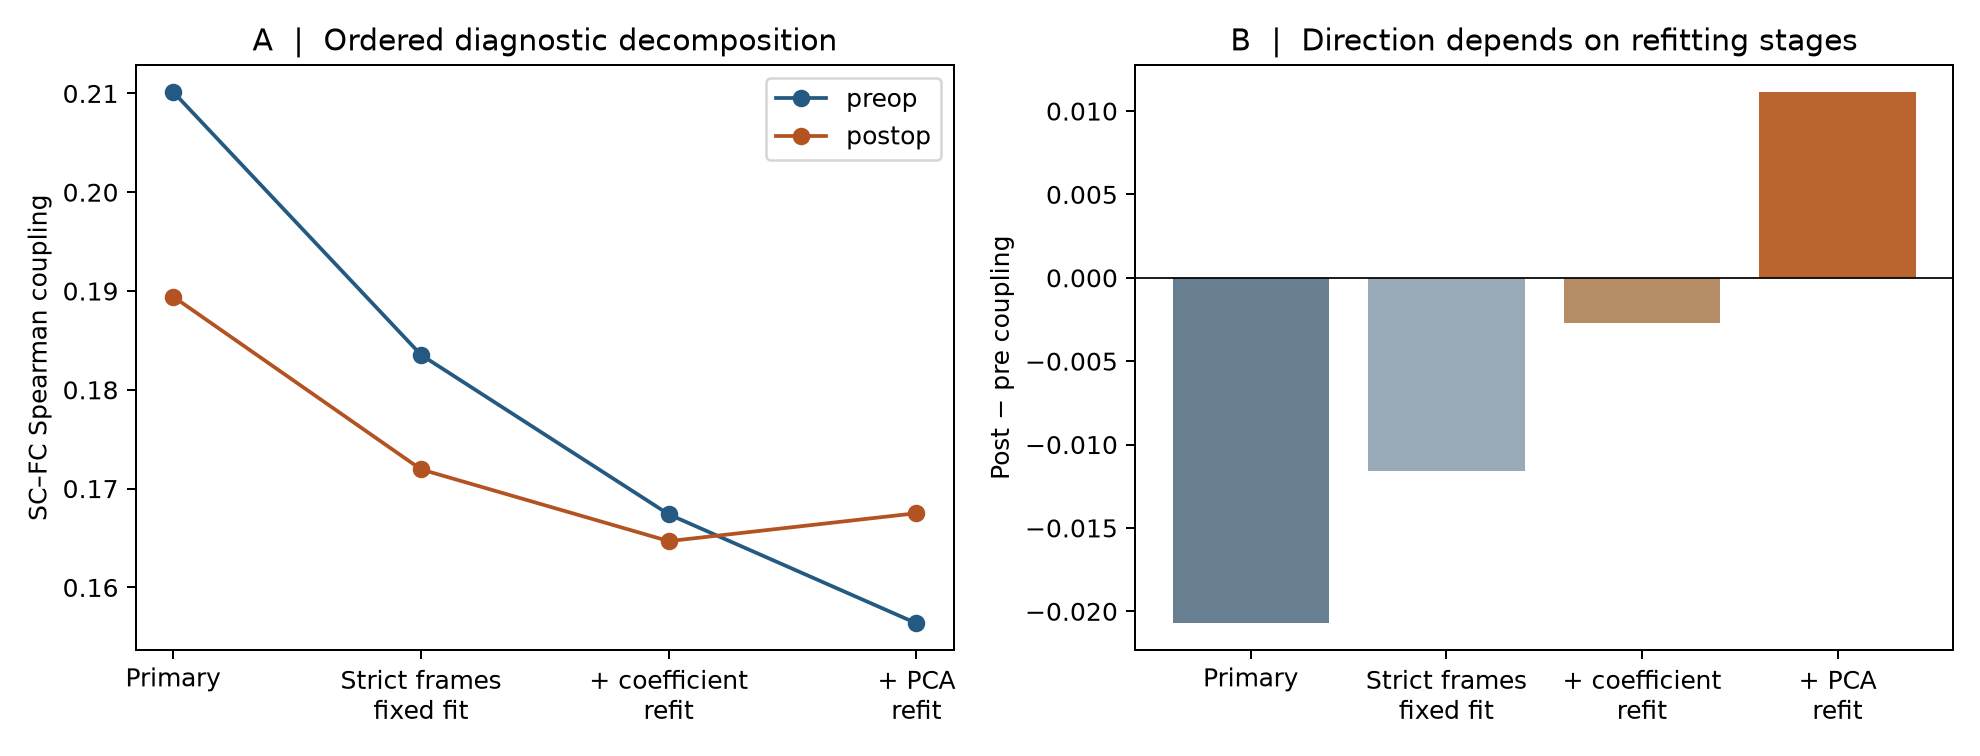
\includegraphics[width=\linewidth]{censoring_decomposition.png}
\caption{Frame restriction and two refitting stages move the contrast across zero. Increments depend on the displayed order and are not causal percentages.}\label{fig:censordecomp}\end{figure}

With 68 frames and full refitting in both sessions, primary-pool median contrasts remain negative under duration, FD and half matching ($-0.0199$, $-0.0215$, $-0.0240$). Strict-pool medians instead vary: $-0.0069$ for duration alone, $-0.0135$ for duration plus FD, but $+0.0101$ with half matching. Every fully refitted central range spans zero (Table~\ref{tab:censormatch}, Fig.~\ref{fig:censormatch}). With the primary fit frozen, all six medians are negative. The original unequal-duration strict increase therefore is not a stable contrast after matched selection, nor can unequal duration alone explain all controls.

\begin{table}[H]\centering\scriptsize\setlength{\tabcolsep}{4pt}\begin{tabular}{lllrrr}
\toprule
Pool & Matching & Fit & Median $\Delta\rho$ & Central 95\% spread & $\Delta>0$ (\%) \\
\midrule
Primary & Duration & Frozen & -0.0239 & [-0.0581, +0.0110] & 11.0 \\
Primary & Duration & Refitted & -0.0199 & [-0.0744, +0.0440] & 26.0 \\
Primary & Duration + FD & Frozen & -0.0287 & [-0.0629, -0.0005] & 2.0 \\
Primary & Duration + FD & Refitted & -0.0215 & [-0.0771, +0.0399] & 23.0 \\
Primary & Duration + FD + half & Frozen & -0.0304 & [-0.0643, -0.0001] & 2.5 \\
Primary & Duration + FD + half & Refitted & -0.0240 & [-0.0897, +0.0273] & 20.5 \\
Strict & Duration & Frozen & -0.0166 & [-0.0324, -0.0016] & 1.5 \\
Strict & Duration & Refitted & -0.0069 & [-0.0389, +0.0246] & 35.5 \\
Strict & Duration + FD & Frozen & -0.0231 & [-0.0366, -0.0066] & 0.0 \\
Strict & Duration + FD & Refitted & -0.0135 & [-0.0439, +0.0144] & 17.5 \\
Strict & Duration + FD + half & Frozen & -0.0173 & [-0.0289, -0.0073] & 0.0 \\
Strict & Duration + FD + half & Refitted & +0.0101 & [-0.0107, +0.0347] & 80.0 \\
\bottomrule
\end{tabular}

\caption{Two hundred draws per protocol, 68 frames/session; $\Delta\rho=\rho_{post}-\rho_{pre}$. Ranges and positive-draw fractions are conditional sampling-design summaries, not confidence intervals, effect probabilities or significance tests. Frozen means both primary PCs and coefficients fixed; refitted means all tissue preprocessing, PCA and final regression fitted on selected frames.}\label{tab:censormatch}\end{table}
\begin{figure}[H]\centering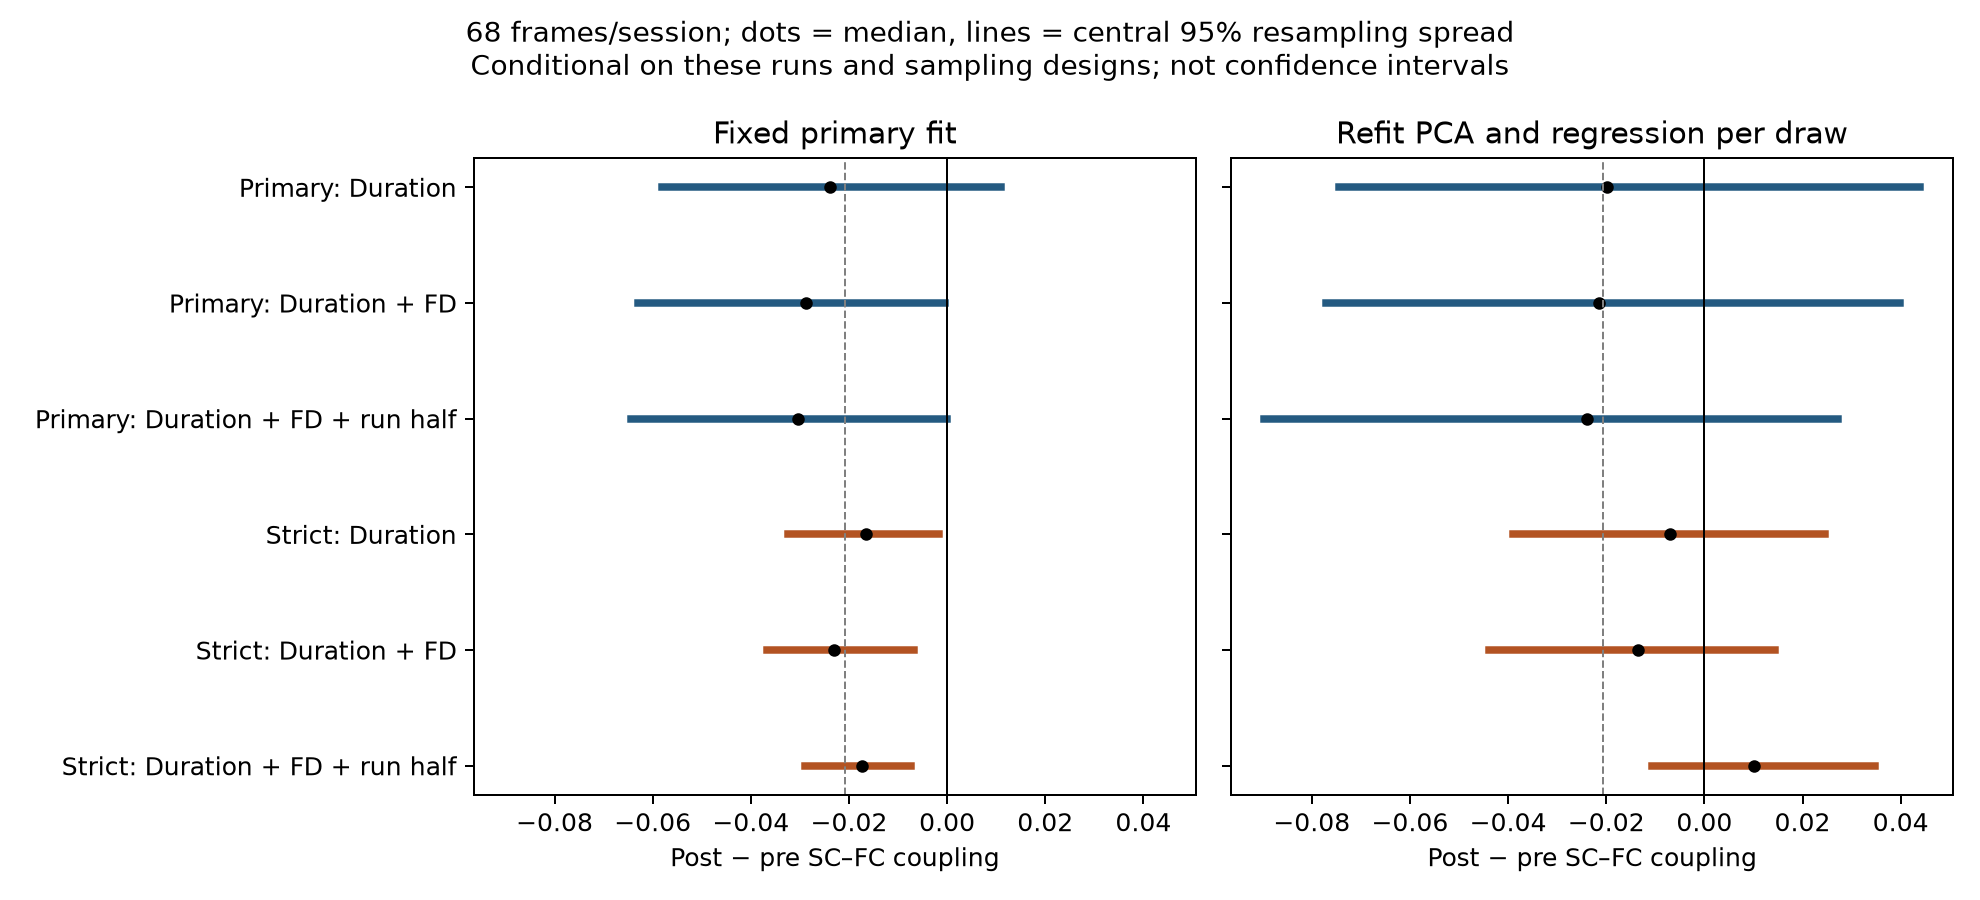
\includegraphics[width=\linewidth]{censoring_matching.png}
\caption{Matched conditional coupling distributions, own-session SC support/weights. Dots mark medians and bars central 95\% resampling spread; the dashed line is the primary full-sample contrast. Controls select distinct frame populations. These spreads do not capture repeated acquisitions or participant uncertainty.}\label{fig:censormatch}\end{figure}

Matching substantially improves FD balance (Table~\ref{tab:censorbalance}); every matched draw has absolute SMD below 0.070 and maximum paired gap at most 0.015 mm. Strict FD-only matching selects a median 40 postoperative first-half frames, versus 46 preoperatively. Joint half matching forces 46 in each session, but still leaves median postoperative third counts 32/22.5/13 versus 35/12/21 preoperatively. Its contrast switches from a frozen-fit median $-0.0173$ to a refitted $+0.0101$. Thus coarse time selection and nuisance refitting remain consequential even after FD/frame-count balance. This is compatible with temporal signal heterogeneity and unstable low-df projection; it does not independently establish either neural state changes or residual artifact as their cause.

\begin{table}[H]\centering\scriptsize\setlength{\tabcolsep}{4pt}\begin{tabular}{llrrrr}
\toprule
Pool & Matching & Med. $|$SMD$|$ & Max. $|$SMD$|$ & Med. $W_1$ (mm) & Med. $\Delta n_{half1}$ \\
\midrule
Primary & Duration & 0.356 & 0.753 & 0.0347 & +2 \\
Primary & Duration + FD & 0.020 & 0.052 & 0.0054 & +0 \\
Primary & Duration + FD + half & 0.015 & 0.039 & 0.0051 & +0 \\
Strict & Duration & 0.169 & 0.356 & 0.0087 & -6 \\
Strict & Duration + FD & 0.013 & 0.069 & 0.0033 & -6 \\
Strict & Duration + FD + half & 0.013 & 0.058 & 0.0037 & +0 \\
\bottomrule
\end{tabular}

\caption{Balance for the same saved draws in both fitting modes. SMD is the retained-FD mean difference divided by the pooled SD; $W_1$ is the Wasserstein distance between retained-FD distributions. $\Delta n_{half1}$ is post-minus-pre first-half count. Zero counts are exact in every half-matched draw; equal FD does not imply equal physiology, fragmentation or serial dependence.}\label{tab:censorbalance}\end{table}

The coupling definition also matters. Only 1,071 nonzero SC edges are common to the 1,515/1,559 own-session supports. On this fixed intersection with session-specific weights, both primary and strict contrasts are negative ($-0.0402$ and $-0.0376$; Table~\ref{tab:censorsupport}); all matched fully refitted median contrasts on common support are negative as well. Fixing preoperative weights on that intersection instead gives full-sample contrasts $+0.0064$ and $+0.0019$. These controls show dependence on structural reference and edge population, not evidence that one reference reveals neural ground truth. Changes in reconstructed SC may contain anatomical and tractography contributions.

\begin{table}[H]\centering\small\begin{tabular}{llrrr}
\toprule
Frames/fit & SC reference & $\rho$ pre & $\rho$ post & $\Delta\rho$ \\
\midrule
Primary & Own SC support/weights & 0.2101 & 0.1894 & -0.0207 \\
Primary & Common support, own weights & 0.2031 & 0.1630 & -0.0402 \\
Primary & Common support, fixed pre SC & 0.2031 & 0.2095 & +0.0064 \\
Strict FD & Own SC support/weights & 0.1564 & 0.1675 & +0.0111 \\
Strict FD & Common support, own weights & 0.1658 & 0.1282 & -0.0376 \\
Strict FD & Common support, fixed pre SC & 0.1658 & 0.1676 & +0.0019 \\
\bottomrule
\end{tabular}

\caption{Changing the SC support/reference while leaving FC fixed changes the question. Fixed preoperative SC measures alignment of each FC matrix with one structural reference; own-session SC measures association of each session's reconstructed pair.}\label{tab:censorsupport}\end{table}

We retain the existing anatomical5/FD0.5 primary recommendation for its stated methodological rationale. The direction of longitudinal SC--FC coupling is explicitly unresolved across censoring, nuisance fitting and SC-reference controls. Thresholds or reference matrices must not be selected from a preferred sign or agreement with cognition.

\subsection{Historical sensitivity: edges and networks of the original reversal}\label{sec:edgeresults}
Here SC means original seed-160 own support throughout; these terms are not current primary consensus results. The own-SC reversal shift is $R=+0.0318647$: strict censoring/refitting changes the longitudinal contrast from $-0.0207203$ to $+0.0111444$. The 2,003-edge union comprises 1,071 shared edges, 444 pre-op-only and 488 post-op-only edges. This partitions structural reconstruction support, not biological tract survival. The exact global-rank accounting assigns $+0.02437$ to pre-op-only edges, $+0.00833$ to shared edges and $-0.00084$ to post-op-only edges (Table~\ref{tab:edgesupport}, Fig.~\ref{fig:edgesupport}). These are signed terms with cancellation, not proportions of neural variance explained.

\begin{table}[H]\centering\footnotesize\setlength{\tabcolsep}{4pt}\begin{tabular}{lrrrrr}
\toprule
SC support & Edges & $\Delta$ primary & $\Delta$ strict & $R$ term & Median counts pre/post \\
\midrule
Shared SC & 1071 & -0.0266 & -0.0182 & +0.0083 & 5 / 6 \\
Pre-op-only SC & 444 & -0.0554 & -0.0310 & +0.0244 & 2 / -- \\
Post-op-only SC & 488 & +0.0612 & +0.0604 & -0.0008 & -- / 2 \\
\bottomrule
\end{tabular}

\caption{Exact additive contributions to the original longitudinal contrasts and their strict-minus-primary difference $R$. Shared terms use global ranks within each full own-SC support, not ranks recomputed on shared edges alone. A dash in median counts indicates absent SC in that session.}\label{tab:edgesupport}\end{table}
\begin{figure}[H]\centering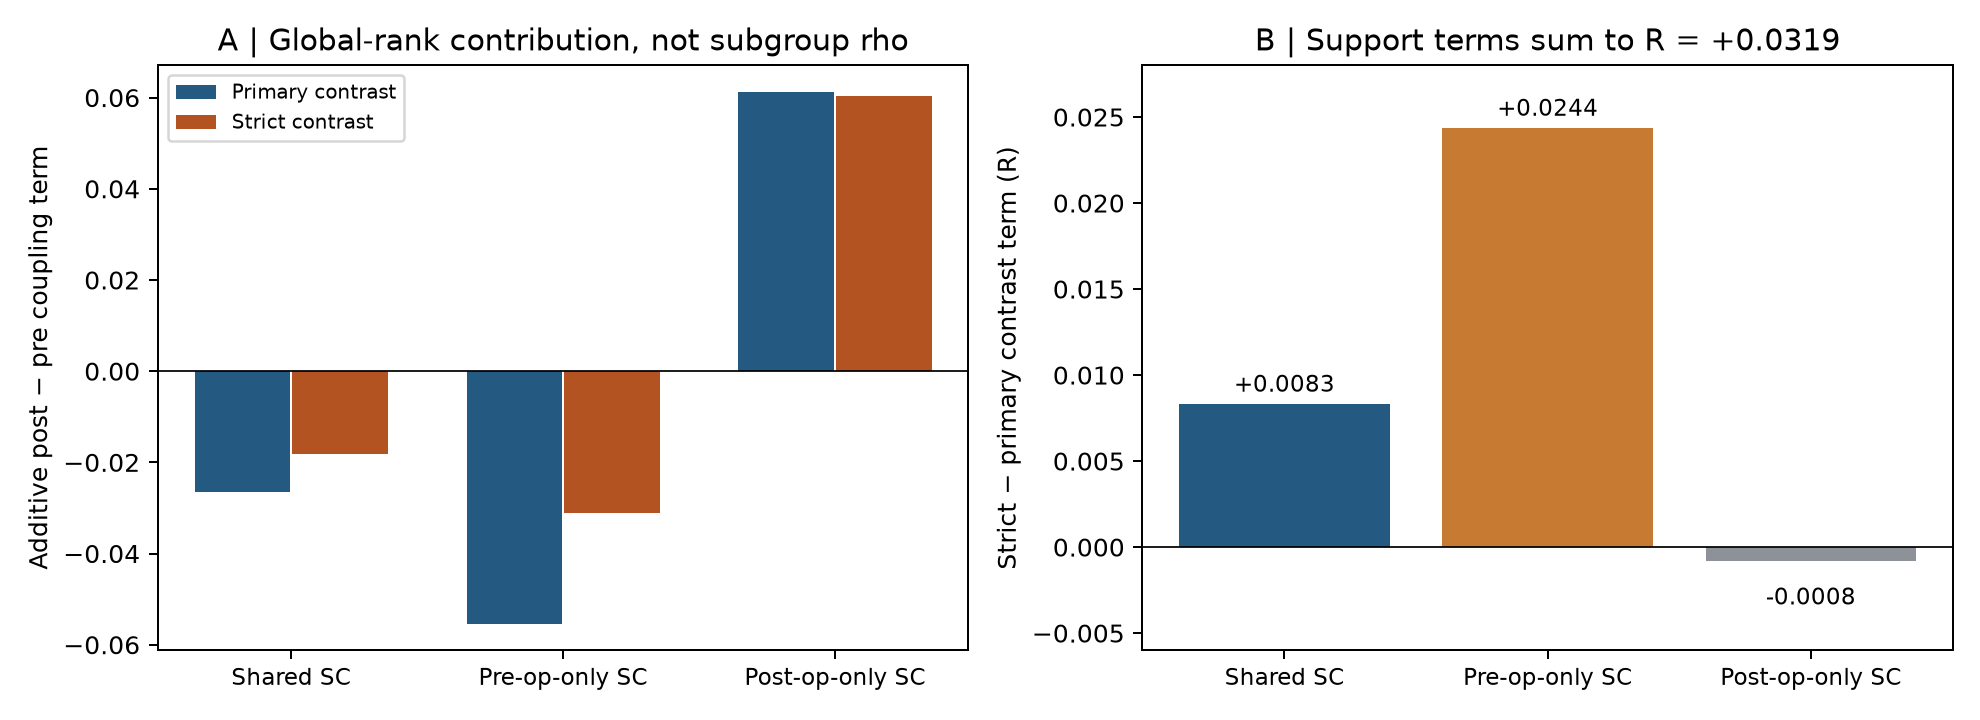
\includegraphics[width=\linewidth]{edge_driver_support.png}
\caption{Support-group rank accounting. Left: terms sum to the primary/strict post-minus-pre contrasts. Right: their differences sum to $R$. No subgroup coefficient is being averaged, and no independent biological effect is assigned to a group.}\label{fig:edgesupport}\end{figure}

Pre-/post-op-only SC counts have median 2, with 61.9\%/66.4\% containing one or two streamlines; the corresponding fractions among shared edges are 29.1\%/28.3\% (median counts 5/6). In the pre-only group, mean measured FC rises from 0.1046 to 0.1338 and mean relative FC rank from 0.4293 to 0.4543 under strict denoising. Its positive pooled preoperative coupling contribution consequently shrinks from 0.05540 to 0.03102. These low-SC edges become less uniformly low-FC in the full ranking; both within-group covariance and between-group rank-location terms change. The source inventory contains all intermediate-stage terms. Low counts and session-specific presence are conditional on tractography/endpoint assignment; neither proves invalidity or anatomical loss.

The largest positive network-pair terms are Default--SomMot ($+0.01237$), Default--SalVentAttn ($+0.00896$) and Default--Limbic ($+0.00644$), with contributions from all three support classes. Within-Vis and within-SomMot also contribute positively. Within-Default ($-0.00700$), Vis--SomMot ($-0.00593$), DorsAttn--SomMot ($-0.00492$) and Cont--SomMot ($-0.00490$) oppose the shift (Table~\ref{tab:edgenetworks}, Fig.~\ref{fig:edgenetworks}). Cross-network and within-network Default terms therefore differ in sign. Group sizes and SC/FC rank distributions affect these totals; atlas labels do not establish a patient-specific functional or cognitive mechanism.

\begin{table}[H]\centering\footnotesize\setlength{\tabcolsep}{4pt}\begin{tabular}{lrrrrr}
\toprule
Network pair & Edges & Shared & Pre-only & Post-only & Total $R$ term \\
\midrule
Default--SomMot & 103 & +0.0044 & +0.0060 & +0.0020 & +0.0124 \\
Default--SalVentAttn & 129 & +0.0046 & +0.0020 & +0.0024 & +0.0090 \\
Default--Limbic & 71 & +0.0023 & +0.0020 & +0.0021 & +0.0064 \\
Vis--Vis & 98 & +0.0028 & +0.0018 & +0.0018 & +0.0063 \\
SomMot--SomMot & 65 & +0.0035 & +0.0015 & +0.0011 & +0.0061 \\
Default--Default & 118 & -0.0035 & -0.0022 & -0.0013 & -0.0070 \\
SomMot--Vis & 45 & -0.0037 & -0.0014 & -0.0008 & -0.0059 \\
DorsAttn--SomMot & 121 & -0.0048 & +0.0006 & -0.0007 & -0.0049 \\
\bottomrule
\end{tabular}

\caption{Five largest positive and three largest negative unordered network-pair terms. Columns partition each pair by SC support and sum to its total $R$ contribution. All 28 pairs and per-edge averages are exported.}\label{tab:edgenetworks}\end{table}
\begin{figure}[H]\centering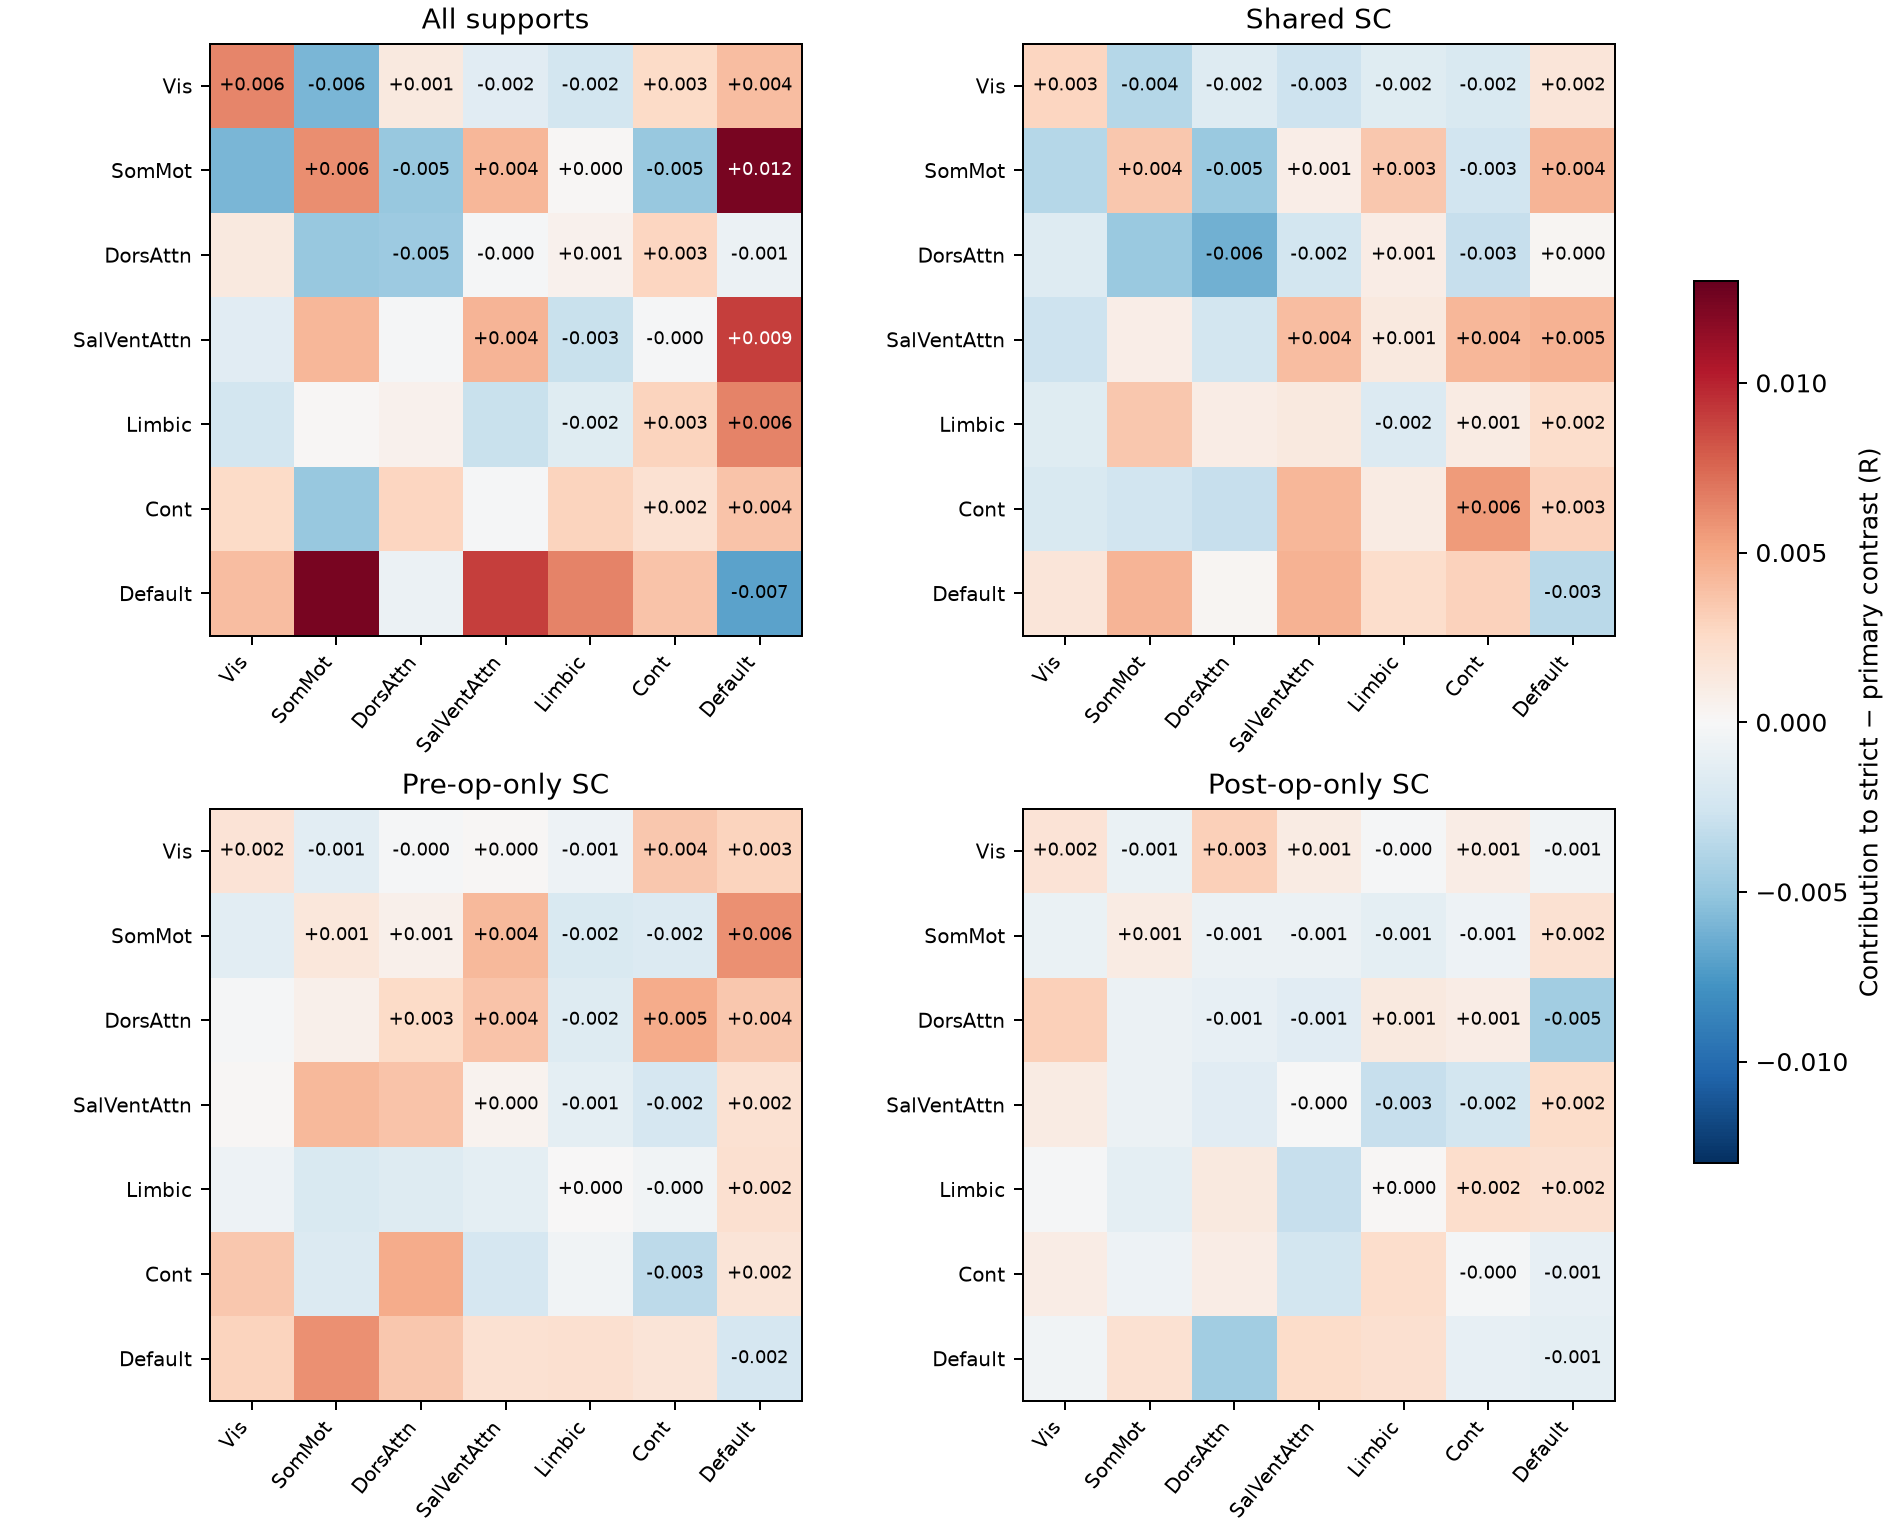
\includegraphics[width=.96\linewidth]{edge_driver_networks.png}
\caption{Network-pair contributions to $R$, separated by support using one colour scale. Each unordered pair is displayed symmetrically and counted once in sums. Numbers appear in the upper triangle; the diagonal denotes within-network edges. These are signed accounting terms, not FC matrices or probabilities of injury.}\label{fig:edgenetworks}\end{figure}

Individual terms are heterogeneous (Table~\ref{tab:edgeindividuals}). The largest positive term is edge 21--42, LH\_DorsAttn\_Post\_6 to LH\_Default\_PFC\_1, pre-op-only with one assigned streamline ($r_e=+0.00277$). The largest negative term is shared edge 16--35, LH\_DorsAttn\_Post\_1 to LH\_Cont\_PFCl\_1 ($-0.00287$). Large terms of opposite signs can occur within one network pair. Across all edges, positive terms total $+0.41647$ and negative terms $-0.38461$, leaving the much smaller net $R$. Neither a single edge nor one positive pair describes this cancellation.

\begin{table}[H]\centering\footnotesize\setlength{\tabcolsep}{4pt}\begin{tabular}{p{.46\linewidth}lrr}
\toprule
Node IDs and Schaefer100 atlas labels & SC support & Counts pre/post & $10^3 r_e$ \\
\midrule
{\ttfamily 21: LH\_\allowbreak{}DorsAttn\_\allowbreak{}Post\_\allowbreak{}6}\newline {\ttfamily 42: LH\_\allowbreak{}Default\_\allowbreak{}PFC\_\allowbreak{}1} & Pre-only & 1 / 0 & +2.773 \\
{\ttfamily 34: LH\_\allowbreak{}Cont\_\allowbreak{}Par\_\allowbreak{}1}\newline {\ttfamily 43: LH\_\allowbreak{}Default\_\allowbreak{}PFC\_\allowbreak{}2} & Shared & 1 / 9 & +2.583 \\
{\ttfamily 21: LH\_\allowbreak{}DorsAttn\_\allowbreak{}Post\_\allowbreak{}6}\newline {\ttfamily 37: LH\_\allowbreak{}Cont\_\allowbreak{}Cing\_\allowbreak{}1} & Shared & 1 / 6 & +2.418 \\
{\ttfamily 32: LH\_\allowbreak{}Limbic\_\allowbreak{}TempPole\_\allowbreak{}1}\newline {\ttfamily 42: LH\_\allowbreak{}Default\_\allowbreak{}PFC\_\allowbreak{}1} & Shared & 27 / 45 & +2.400 \\
{\ttfamily 16: LH\_\allowbreak{}DorsAttn\_\allowbreak{}Post\_\allowbreak{}1}\newline {\ttfamily 35: LH\_\allowbreak{}Cont\_\allowbreak{}PFCl\_\allowbreak{}1} & Shared & 50 / 62 & -2.873 \\
{\ttfamily 68: RH\_\allowbreak{}DorsAttn\_\allowbreak{}Post\_\allowbreak{}2}\newline {\ttfamily 83: RH\_\allowbreak{}Cont\_\allowbreak{}PFCl\_\allowbreak{}1} & Shared & 1 / 1 & -2.716 \\
{\ttfamily 53: RH\_\allowbreak{}Vis\_\allowbreak{}3}\newline {\ttfamily 86: RH\_\allowbreak{}Cont\_\allowbreak{}PFCl\_\allowbreak{}4} & Shared & 26 / 7 & -2.469 \\
{\ttfamily 90: RH\_\allowbreak{}Default\_\allowbreak{}Par\_\allowbreak{}1}\newline {\ttfamily 95: RH\_\allowbreak{}Default\_\allowbreak{}PFCv\_\allowbreak{}2} & Shared & 1 / 7 & -2.398 \\
\bottomrule
\end{tabular}

\caption{Four largest positive and four largest negative individual $r_e$ terms. IDs refer to the fixed Schaefer100 node table; labels omit the common \texttt{7Networks} prefix. Counts 0 indicate absent reconstructed SC, not missing FC. Terms depend on the full pooled ranking. The complete 2,003-edge inventory is supplied as CSV.}\label{tab:edgeindividuals}\end{table}

Every one of 2,003 single-edge deletions preserves the original negative-primary/positive-strict contrast. Deleting the ten largest positive terms jointly makes strict $\Delta$ slightly negative ($-0.00109$), but this set is selected from the same observations and is not a validated set of causal pathways. Group deletion illustrates why additive accounting and removal differ (Table~\ref{tab:edgedeletions}). Removing pre-only edges leaves $\Delta=-0.0137/+0.0017$ (primary/strict); removing post-only edges gives $-0.0472/-0.0282$, despite that group's small direct $R$ term. Removing both session-specific supports gives the shared-only negative contrasts. Reranking the survivors changes context and normalization.

Removing all Default-incident edges makes both contrasts positive ($+0.0367/+0.0393$), reducing the reversal shift to $+0.0026$. Removing SalVentAttn-, Limbic- or Cont-incident edges instead makes both contrasts negative (Fig.~\ref{fig:edgedeletions}). Thus neither one edge nor one support class/network has a unique necessary biological interpretation. Network-incident deletion sets overlap and their effects cannot be summed.

\begin{table}[H]\centering\footnotesize\setlength{\tabcolsep}{4pt}\begin{tabular}{lrrrr}
\toprule
Edges removed & Union edges & $\Delta$ primary & $\Delta$ strict & $R$ after removal \\
\midrule
None (original) & 0 & -0.0207 & +0.0111 & +0.0319 \\
All shared SC & 1071 & -0.0609 & -0.0107 & +0.0502 \\
All pre-op-only SC & 444 & -0.0137 & +0.0017 & +0.0154 \\
All post-op-only SC & 488 & -0.0472 & -0.0282 & +0.0190 \\
Both session-specific SC groups & 932 & -0.0402 & -0.0376 & +0.0026 \\
Vis incident edges & 445 & -0.0191 & +0.0170 & +0.0362 \\
SomMot incident edges & 511 & -0.0215 & +0.0131 & +0.0346 \\
DorsAttn incident edges & 578 & -0.0383 & +0.0212 & +0.0596 \\
SalVentAttn incident edges & 475 & -0.0369 & -0.0158 & +0.0210 \\
Limbic incident edges & 247 & -0.0342 & -0.0056 & +0.0286 \\
Cont incident edges & 522 & -0.0338 & -0.0031 & +0.0307 \\
Default incident edges & 813 & +0.0367 & +0.0393 & +0.0026 \\
Top 10 positive edge terms & 10 & -0.0108 & -0.0011 & +0.0097 \\
\bottomrule
\end{tabular}

\caption{Reranked deletion stress tests. Every row recalculates both sessions' SC/FC ranks and normalizers on remaining positive-SC edges; results are not original contrast minus the deleted group's additive term. Network-incident sets overlap. Top-ten selection is post hoc.}\label{tab:edgedeletions}\end{table}
\begin{figure}[H]\centering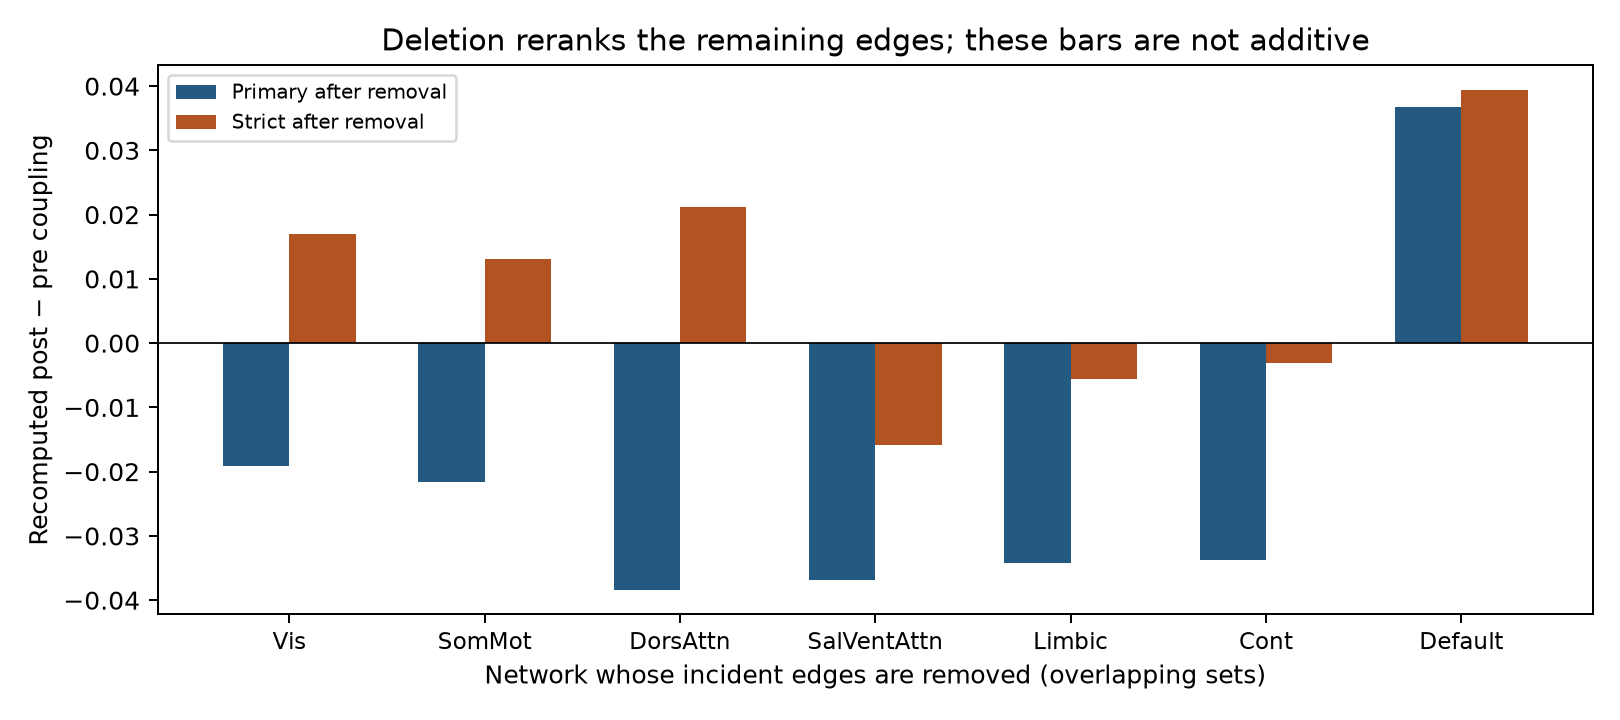
\includegraphics[width=\linewidth]{edge_driver_deletions.png}
\caption{Primary/strict longitudinal contrasts after deleting all edges incident on the named network. All remaining ranks are recomputed. Overlapping deletions yield different signs, limiting any single-network explanation of the original reversal.}\label{fig:edgedeletions}\end{figure}

Matched replay further changes the localization (Table~\ref{tab:edgematched}). All strict-pool full refits have the same pre-only term, $-0.03102$, because every draw retains the same 68 preoperative frames. Moving from duration+FD to duration+FD+half matching changes the shared-edge mean term from $-0.03272$ to $-0.01395$, and post-only from $+0.05032$ to $+0.05560$. The total mean shifts from $-0.01343$ to $+0.01063$, mostly through shared edges. These are means of matched contrasts, distinct from the medians in Table~\ref{tab:censormatch}. The same-frame refitted-minus-frozen pre-only effect is $+0.01782$ for all strict designs, whereas the shared effect changes from $-0.00489$ to $+0.01224$ under half matching. At network-pair level, the largest positive half-versus-FD mean design shift is Cont--SomMot ($+0.00408$), a pair opposing the original full-sample $R$. Different diagnostic questions therefore identify different leading terms.

\begin{table}[H]\centering\footnotesize\setlength{\tabcolsep}{4pt}\begin{tabular}{lrrrr}
\toprule
Strict-pool matching & Shared term & Pre-only term & Post-only term & Mean $\Delta$ \\
\midrule
Duration & -0.0250 & -0.0310 & +0.0493 & -0.0067 \\
Duration + FD & -0.0327 & -0.0310 & +0.0503 & -0.0134 \\
Duration + FD + half & -0.0140 & -0.0310 & +0.0556 & +0.0106 \\
\bottomrule
\end{tabular}

\caption{Mean support contributions to the strict-pool matched post-minus-pre contrast under full nuisance refitting (200 draws, 68 frames/session). Disjoint support means sum to the mean total; marginal medians/quantiles do not. Conditional spreads, available in the notebook/CSV, are not confidence intervals or surgical-effect probabilities.}\label{tab:edgematched}\end{table}

Endpoint proximity does not confine the positive shift to the lesion footprint: edges with either atlas centroid within 10 mm contribute $-0.01463$ (719 edges), versus $+0.04649$ when both endpoints are farther away (1,284). This is an endpoint partition, not a test of tract traversal or cavity injury. Taken together, the analysis localizes a distributed methodological sensitivity, retaining the existing primary denoising choice and the unresolved longitudinal coupling direction. No new cognitive or quality-of-life mechanism follows from these edge/network rankings.

\subsection{Reliability of low-count and session-specific structural edges}\label{sec:screliabilityresults}
Both seed-160 replays reproduce the original count matrices exactly, including the 26,488/26,421 length-filtered streamlines. Forty new runs then track 1.2 million seed locations in total (20$\times$30,000 per session). They vary seeding within the fixed model and scans, rather than the acquisitions or anatomical assumptions. All 4,950 possible cortical pairs are retained in the reliability inventory.

Original one-streamline edges have median nonzero detection fractions 0.55/0.50 across new pre/post runs, versus 0.85/0.80 for original count two (Table~\ref{tab:screpeatcounts}). Original counts at least ten have median detection 1.00 in both sessions. Median count CVs for original singletons are 1.12/1.13, including zero-count runs whenever mean count is positive. Stable nonzero detection does not imply stable passage of an aggressive higher count cutoff.

\begin{table}[H]\centering\small\begin{tabular}{lrrr}
\toprule
Original count & Edges pre/post & Median detection pre/post & Median CV pre/post \\
\midrule
1 & 379 / 424 & 0.55 / 0.50 & 1.12 / 1.13 \\
2 & 208 / 203 & 0.85 / 0.80 & 0.73 / 0.73 \\
3--4 & 277 / 234 & 0.95 / 0.95 & 0.53 / 0.53 \\
5--9 & 262 / 270 & 1.00 / 1.00 & 0.37 / 0.40 \\
$\geq10$ & 389 / 428 & 1.00 / 1.00 & 0.18 / 0.19 \\
\bottomrule
\end{tabular}

\caption{Conditional seed stability by original count. Occurrence means nonzero count in 20 new runs; CV is SD/mean count, including zeros but omitting undefined all-zero CVs. These are edge-distribution summaries, not uncertainty intervals for true anatomical connectivity.}\label{tab:screpeatcounts}\end{table}

Among 444 original pre-op-only edges, 322 (72.5\%) reappear at least once post-op; among 488 original post-op-only edges, 342 (70.1\%) reappear pre-op. Only 31/24 reach 80\% occurrence in those previously absent sessions. Thus ``ever rediscovered'' and consistently present are different claims. Original support labels often fail to persist under further sampling, while low occurrence in the opposite session still does not prove anatomical absence (Table~\ref{tab:screpeatsupport}, Fig.~\ref{fig:screpeatdetection}).

\begin{table}[H]\centering\footnotesize\setlength{\tabcolsep}{4pt}\begin{tabular}{lrrrrrr}
\toprule
Original support & Edges & Med. pre $p$ & Med. post $p$ & Ever pre & Ever post & Both $p\geq.8$ \\
\midrule
Shared & 1071 & 1.00 & 1.00 & 1069 & 1068 & 780 \\
Pre-op-only & 444 & 0.80 & 0.15 & 439 & 322 & 25 \\
Post-op-only & 488 & 0.10 & 0.70 & 342 & 478 & 17 \\
Absent in both & 2947 & 0.00 & 0.00 & 731 & 820 & 1 \\
\bottomrule
\end{tabular}

\caption{Original support versus new occurrence at count $\geq1$. Median $p$ is the fraction of 20 runs containing the edge. ``Ever'' means at least one hit. The last column requires occurrence $\geq.8$ in both sessions, a different support definition from original sharing.}\label{tab:screpeatsupport}\end{table}
\begin{figure}[H]\centering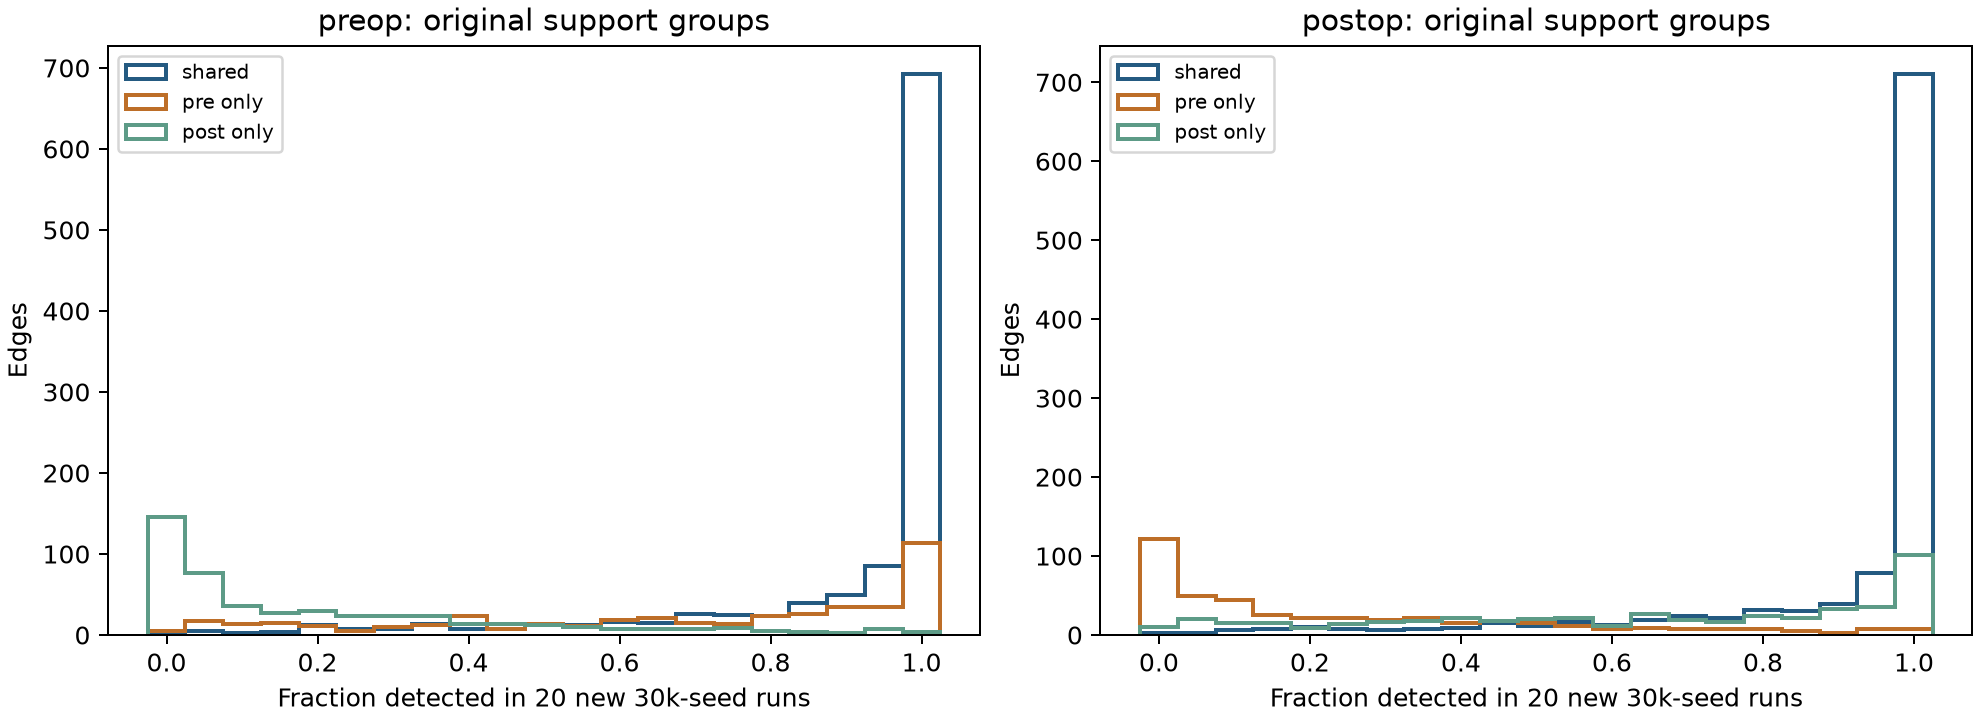
\includegraphics[width=\linewidth]{sc_repeat_detection.png}
\caption{Detection across newly generated tractograms, grouped by original SC support. Edges can be missed in an original session but detected by additional random seeding. All geometry/model settings are held fixed.}\label{fig:screpeatdetection}\end{figure}

\begingroup\clubpenalty=10000
For the original largest positive reversal term, edge 21--42 (one/zero streamlines), repeated nonzero occurrence is 0.15/0.10; mean counts per 30,000 seeds are 0.15/0.15. Its original rank contribution is unchanged, but the reconstruction-presence label is conditional. The complete inventory cross-tabulates original signed reversal terms by 80\% repeat class and preserves their exact total $R=+0.0318647$. First/last-ten consensus Jaccard at $k=1$ is 0.865/0.861 (pre/post). This is split seeding consistency, not validation against known pathways.\par\endgroup

The original pre-only contribution $+0.02437$ is concentrated in 207 edges that fail to reach 80\% occurrence in either session: their signed term is $+0.02412$ (Table~\ref{tab:screpeatclasses}). Other classes contain opposing terms, so this is signed rank accounting rather than a percentage of biological variance. The largest negative original edge, 16--35, is detected in all 20 runs in both sessions; sensitivity is therefore not confined to unstable edges.

\begin{table}[H]\centering\footnotesize\setlength{\tabcolsep}{3pt}\begin{tabular}{lrrrrr}
\toprule
80\% repeat class & Union edges & Original shared & Original pre-only & Original post-only & Total $R$ term \\
\midrule
Both & 822 & +0.0039 & -0.0021 & +0.0014 & +0.0032 \\
Pre-op only & 323 & +0.0093 & +0.0023 & -0.0003 & +0.0112 \\
Post-op only & 316 & -0.0033 & +0.0001 & +0.0011 & -0.0020 \\
Neither & 542 & -0.0016 & +0.0241 & -0.0030 & +0.0195 \\
\bottomrule
\end{tabular}

\caption{Original reversal terms cross-tabulated by new 80\% occurrence class at $k=1$. Counts refer only to the original 2,003-edge union. ``Only'' means the other session is below 80\%, not undetected. Original global ranks are held fixed for this accounting; rows sum to the original $R$.}\label{tab:screpeatclasses}\end{table}

The original own-support coupling contrasts change non-monotonically with count cutoff (Table~\ref{tab:screpeatcoupling}). At $k=2$ both are positive ($+0.00842/+0.03138$, primary/strict); at $k=3$ they are close to zero with opposite ordering ($+0.00103/-0.00207$); at $k=5$ both are negative ($-0.02200/-0.01114$). At $k=10$ both are negative and at $k=20$ both positive. Original common-support contrasts are negative at all six cutoffs. Removing low counts therefore does not produce a single monotone or validated correction to the original reversal. Each cutoff changes the ranked population.

\begin{table}[H]\centering\scriptsize\setlength{\tabcolsep}{3pt}\begin{tabular}{lrrrrrr}
\toprule
Min. count & Edges pre/post & Original $\Delta_P$ & Original $\Delta_S$ & Repeat med. $\Delta_P$ & Repeat med. $\Delta_S$ & Flip fraction \\
\midrule
1 & 1515 / 1559 & -0.0207 & +0.0111 & -0.0004 & +0.0285 & 0.435 \\
2 & 1136 / 1135 & +0.0084 & +0.0314 & -0.0142 & +0.0197 & 0.542 \\
3 & 928 / 932 & +0.0010 & -0.0021 & -0.0060 & +0.0285 & 0.527 \\
5 & 651 / 698 & -0.0220 & -0.0111 & -0.0322 & -0.0024 & 0.343 \\
10 & 389 / 428 & -0.0302 & -0.0839 & -0.0116 & -0.0556 & 0.005 \\
20 & 225 / 219 & +0.0283 & +0.0096 & -0.0105 & -0.0442 & 0.007 \\
\bottomrule
\end{tabular}

\caption{Own-support count-threshold sensitivity with unchanged FC. $\Delta_P$ and $\Delta_S$ are primary/strict post-minus-pre contrasts. Repeat medians use all 400 pre/post run combinations. ``Flip fraction'' is the descriptive fraction with $\Delta_P<0<\Delta_S$, not a probability of a biological effect. Common-support results and empirical ranges are exported.}\label{tab:screpeatcoupling}\end{table}
\begin{figure}[H]\centering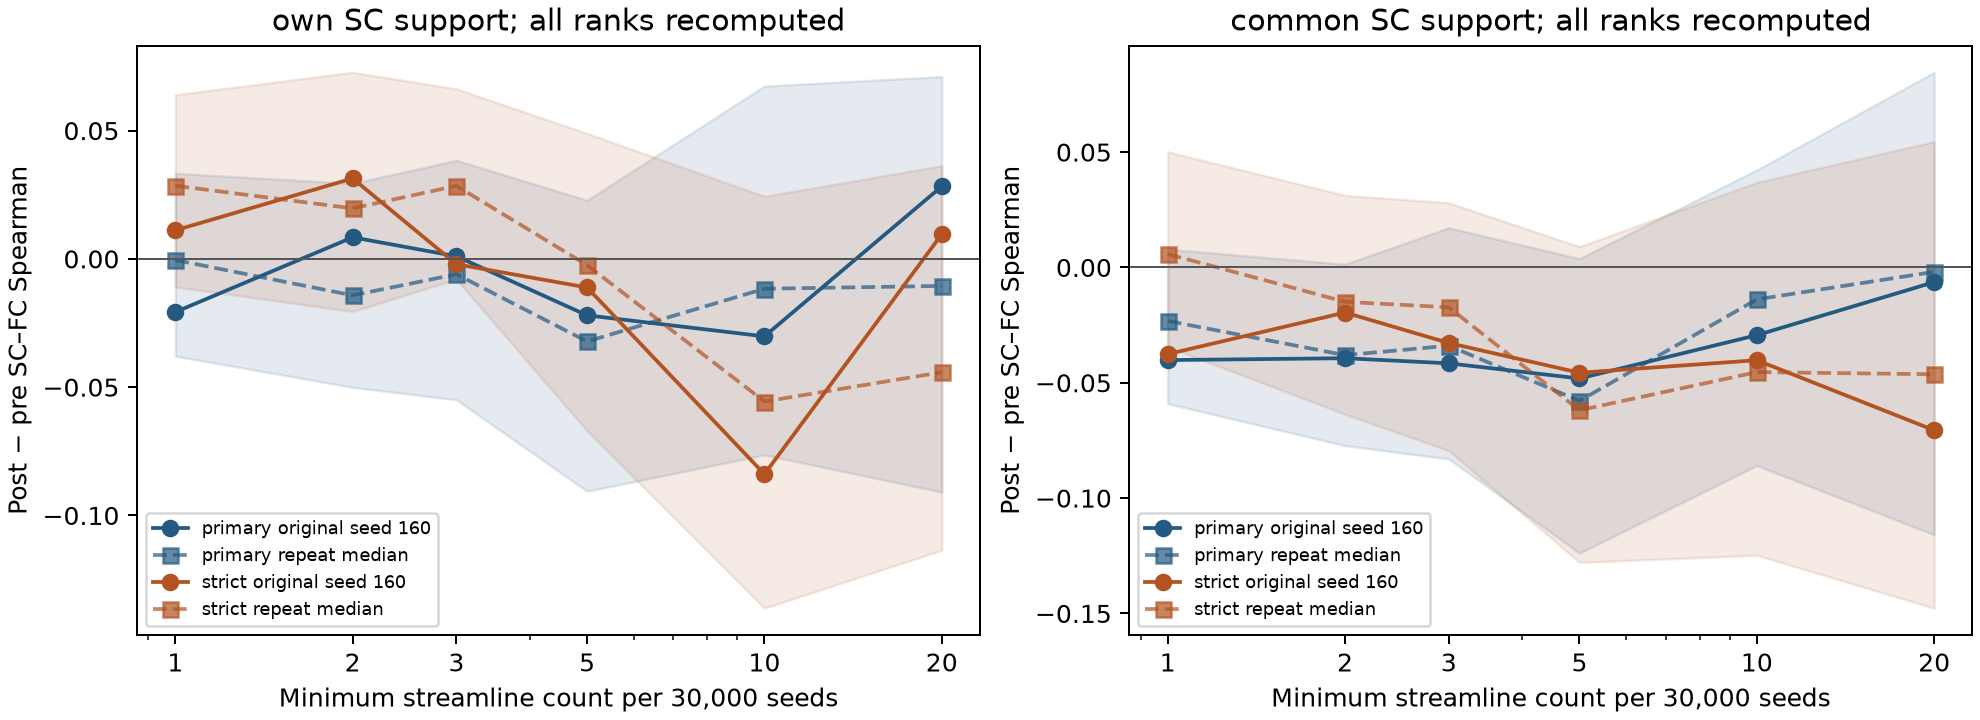
\includegraphics[width=\linewidth]{sc_repeat_coupling.png}
\caption{Count-threshold coupling under original and repeated SC. Shading is the empirical 2.5/97.5-percentile range over dependent run combinations, conditional on fixed FC/scans. Own and common support answer different questions; all ranks are recomputed.}\label{fig:screpeatcoupling}\end{figure}

At $k=1$ with repeated own-support SC, median primary/strict contrasts are -0.00043/+0.02852; their empirical ranges are [-0.03790, +0.03337] and [-0.01090, +0.06403]. The original negative-primary/positive-strict pattern occurs in 174/400 combinations. This quantifies sensitivity to seeding under the same scans and BOLD fits, not independent longitudinal replication. Repeated common-support median contrasts are -0.02317/+0.00579, with both empirical ranges spanning zero. Thus even the original common-only negative point contrasts depend on which tractography run defines the intersection.

At 80\% occurrence and $k=1$, own consensus retains 1160/1163 edges and yields $\Delta_P=-0.00257$, $\Delta_S=+0.02363$. Common consensus retains 823 edges in each session, with contrasts -0.04173/-0.03424. Mean-count weighting also changes SC ranks/ties, so consensus is more than deleting unreliable original edges. Results for every occurrence/cutoff setting are supplied (Table~\ref{tab:screpeatconsensus}, Fig.~\ref{fig:screpeatconsensus}); none is selected from its sign.

\begin{table}[H]\centering\small\begin{tabular}{llrrrr}
\toprule
SC support & Min. occurrence & Edges pre/post & $\Delta_P$ & $\Delta_S$ & $R$ \\
\midrule
own & 0.50 & 1476 / 1491 & -0.0000 & +0.0375 & +0.0375 \\
own & 0.80 & 1160 / 1163 & -0.0026 & +0.0236 & +0.0262 \\
own & 0.95 & 941 / 946 & +0.0033 & +0.0413 & +0.0379 \\
own & 1.00 & 811 / 822 & +0.0166 & +0.0354 & +0.0188 \\
common & 0.50 & 1100 / 1100 & -0.0387 & -0.0005 & +0.0383 \\
common & 0.80 & 823 / 823 & -0.0417 & -0.0342 & +0.0075 \\
common & 0.95 & 659 / 659 & -0.0292 & -0.0177 & +0.0115 \\
common & 1.00 & 551 / 551 & -0.0386 & -0.0370 & +0.0016 \\
\bottomrule
\end{tabular}

\caption{Consensus at count $\geq1$ with mean-count SC weights. Occurrence threshold selects support; it is not a calibrated anatomical confidence. All cutoffs $k=1,2,3,5,10,20$ and network-pair signed terms are exported.}\label{tab:screpeatconsensus}\end{table}
\begin{figure}[H]\centering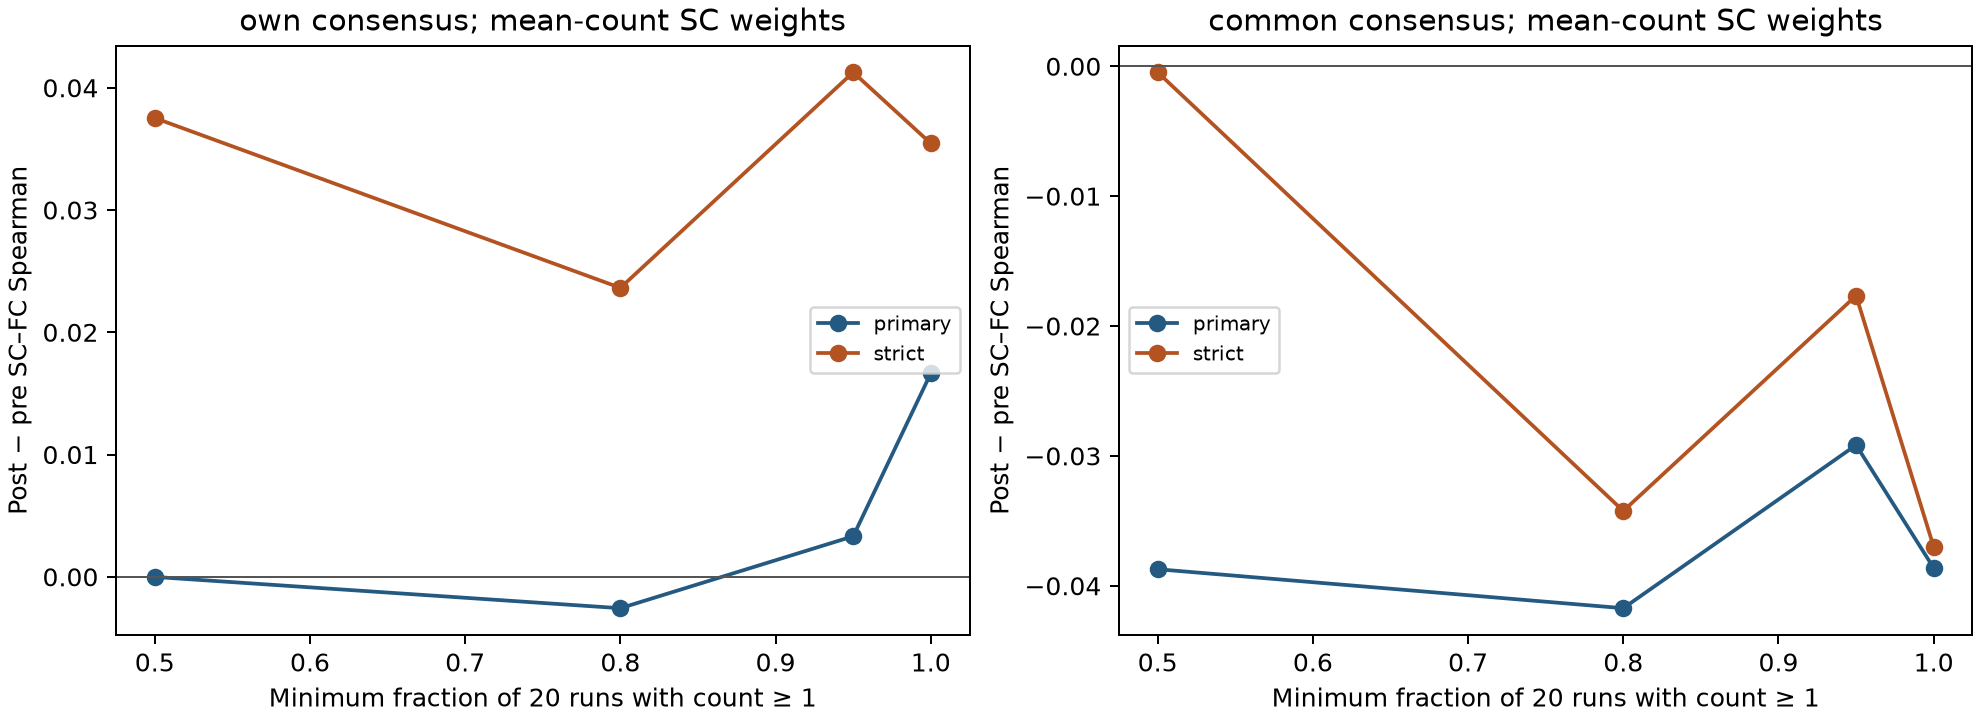
\includegraphics[width=\linewidth]{sc_repeat_consensus.png}
\caption{Consensus fraction sensitivity with primary/strict FC fixed. Own and common supports use the same 20-run mean counts but different edge populations. These curves do not identify a preferred anatomical threshold.}\label{fig:screpeatconsensus}\end{figure}

All 1,200 preceding fully refitted matched draws are reproduced at original $k=1$, and each is evaluated under five fixed SC references (6,000 contrasts; Table~\ref{tab:screpeatmatched}). Under 80\% common consensus, strict-pool FD-matched median $\Delta$ is -0.04797 [-0.08979, -0.01587], versus -0.02217 [-0.05572, +0.00908] with acquisition-half matching. These controls vary FC selection at fixed SC; the repeated-seeding analyses vary SC at fixed FC. Their separate marginal spreads must not be added. Section~\ref{sec:jointresults} evaluates joint perturbations directly under the primary strategy.

\begin{table}[H]\centering\scriptsize\setlength{\tabcolsep}{3pt}\begin{tabular}{lrrr}
\toprule
Fixed SC reference & Duration & Duration + FD & Duration + FD + half \\
\midrule
Original $k\geq1$ & -0.007 [-0.039, +0.025] & -0.013 [-0.044, +0.014] & +0.010 [-0.011, +0.035] \\
Original $k\geq3$ & -0.011 [-0.056, +0.023] & -0.016 [-0.052, +0.019] & +0.010 [-0.021, +0.038] \\
Original $k\geq5$ & -0.021 [-0.067, +0.018] & -0.026 [-0.068, +0.009] & -0.008 [-0.042, +0.021] \\
80\% own consensus & +0.007 [-0.033, +0.042] & +0.001 [-0.032, +0.034] & +0.029 [-0.002, +0.056] \\
80\% common consensus & -0.042 [-0.082, +0.001] & -0.048 [-0.090, -0.016] & -0.022 [-0.056, +0.009] \\
\bottomrule
\end{tabular}

\caption{Strict-pool matched FC under fixed SC references: median [conditional 2.5/97.5 percentiles], 200 draws per cell. All six protocols are retained in the notebook/CSV. These are conditional sampling spreads, not confidence intervals or treatment-effect probabilities.}\label{tab:screpeatmatched}\end{table}

The recommendation in Section~\ref{sec:primaryscmethods} now replaces original single-run SC in the main analyses. Original SC/anatomical5-FD0.5 remains an explicitly labelled historical sensitivity, alongside count cutoffs, alternative consensus and own-support coupling. Repeated support improves the description of conditional reconstruction stability; it cannot calibrate anatomical truth. The longitudinal coupling direction remains unresolved across SC population, SC weights, BOLD selection and nuisance fitting. No newly identified edge or network is assigned a CANTAB or quality-of-life mechanism.

\subsection{Topology, weights and sensitivity}
The historical seed-160 sensitivity in Table~\ref{tab:correction} and Figure~\ref{fig:correction} compares topup/eddy against a matched rigid-only reconstruction with the revised shell-specific model. One maximum weight scale is shared across all four graphs in this comparison; it may differ from the scale for the corrected-only paired results below. Preprocessing differences include downstream EPI-to-T1 registration. Comparing the previous delivery directly with this revision would additionally include the shell-selection change.
\begin{table}[H]\centering\small\begin{tabular}{llrrrr}
\toprule
Session & Processing & Assigned & Binary $E$ & Weighted $E$ & SC--FC $\rho$ \\
\midrule
preop & Topup/eddy & 16258 & 0.5687 & 0.02890 & 0.210 \\
preop & Rigid only & 16521 & 0.5709 & 0.03146 & 0.191 \\
postop & Topup/eddy & 15889 & 0.5733 & 0.02751 & 0.189 \\
postop & Rigid only & 17423 & 0.5711 & 0.02950 & 0.195 \\
\bottomrule
\end{tabular}

\caption{Matched preprocessing comparison at density 0.20. Both variants use identical reconstruction, seeding and endpoint settings. Weighted efficiency uses one scale across all four graphs; coupling uses identical anatomical-primary BOLD FC across structural variants and nonzero SC edges.}\label{tab:correction}\end{table}
\begin{figure}[H]\centering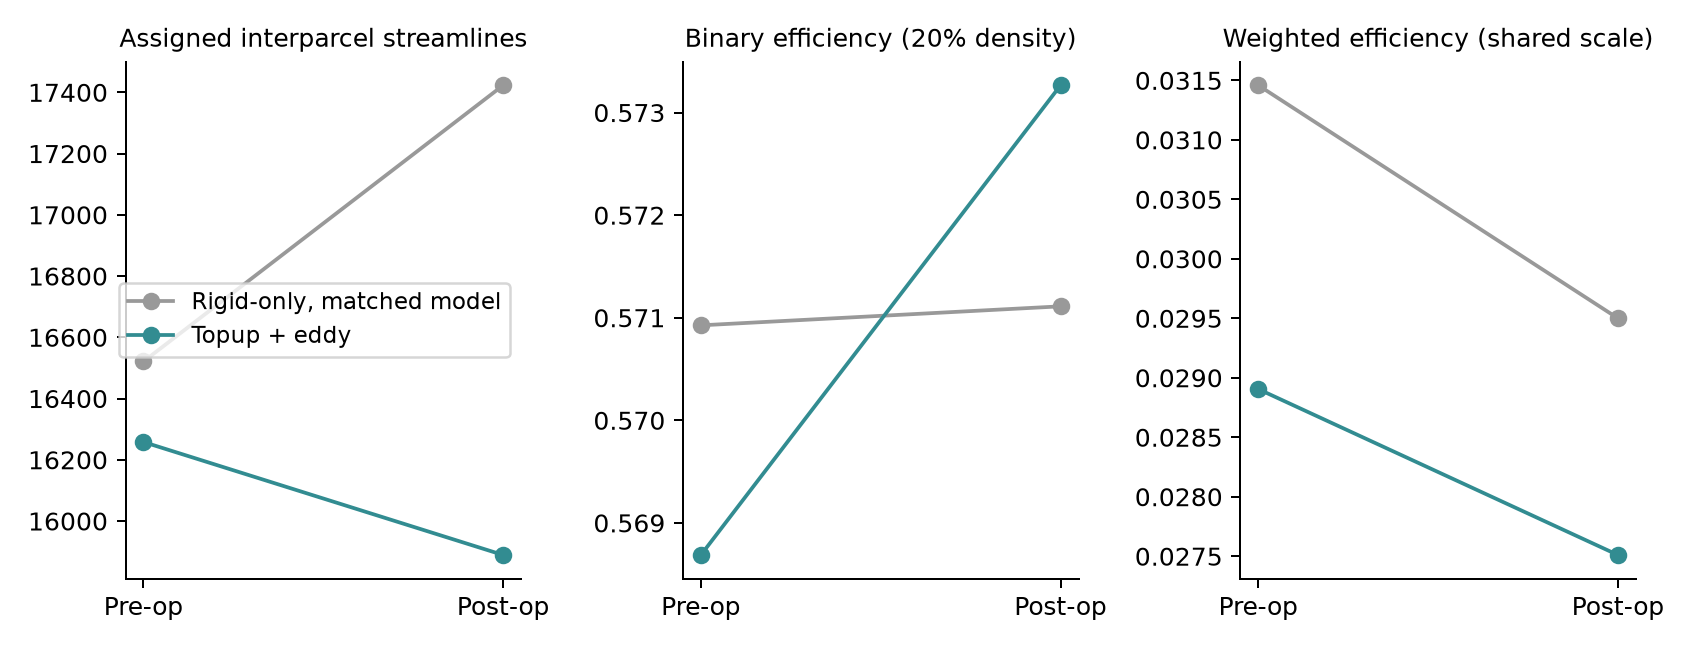
\includegraphics[width=\linewidth]{correction_comparison.png}
\caption{Processing sensitivity of structural yields and graph efficiency. Changes are methodological estimates, not validation against known anatomical connections.}\label{fig:correction}\end{figure}
Assignment yield rose across sessions with rigid-only preprocessing and fell with topup/eddy. The SC comparison holds the newly corrected BOLD FC fixed in both structural variants. Historical single-run corrected-SC coupling was 0.210 and 0.189; differences across structural reconstructions emphasize processing sensitivity.

Using primary own-consensus mean-rate weights at density 0.20, binary SC efficiency was \PreSCBinaryE{} preoperatively and \PostSCBinaryE{} postoperatively. Weighted SC efficiency was \PreSCWeightedE{} and \PostSCWeightedE{} (approximately $\SCWeightedPercentChange\%$). Both SC graphs were connected. These are reconstructed graph differences at one threshold, not demonstrated axonal loss. Positive-FC weighted efficiency was \PreFCWeightedE{} and \PostFCWeightedE{} under primary denoising (Table~\ref{tab:graphs}).
\begin{table}[H]\centering\small\begin{tabular}{llrr}
\toprule
Graph & Metric & Pre-op & Post-op \\
\midrule
SC & edges & 990 & 990 \\
SC & components & 1 & 1 \\
SC & binary global efficiency & 0.569 & 0.571 \\
SC & weighted global efficiency & 0.048 & 0.045 \\
SC & weighted clustering & 0.019 & 0.019 \\
FC positive & edges & 990 & 990 \\
FC positive & components & 1 & 1 \\
FC positive & binary global efficiency & 0.558 & 0.574 \\
FC positive & weighted global efficiency & 0.214 & 0.194 \\
FC positive & weighted clustering & 0.199 & 0.152 \\
\bottomrule
\end{tabular}

\caption{Primary graphs at requested/achieved density 0.20 (990 edges). SC uses own repeat consensus and one shared maximum scale, 101.7 assignments per 10,000 seeds. SC has 100 nodes; FC uses the common valid set. Cross-modality efficiency magnitudes are not directly comparable.}\label{tab:graphs}\end{table}

Table~\ref{tab:primaryscgraphsensitivity} separates weighting and support sensitivities. Rescaling an entire session preserves its within-session rank ordering; replacing session-total fractions by a fixed seed denominator can nevertheless change the longitudinal weighted-efficiency contrast under a shared scale. The unfiltered repeat mean and own consensus have identical weighted efficiency at density 0.20 despite one edge swap in each session: these weak substitutions do not change any weighted shortest-path distance. Identical efficiency therefore does not imply identical graphs. Their full supports and higher-density summaries also differ. Common-consensus graphs saturate at 823 edges (density 0.1663), so their requested 0.20 is not an achieved matched density. Full density, graph and network sensitivity tables are exported and interactive in notebook 03.
\begin{table}[H]\centering\scriptsize\setlength{\tabcolsep}{4pt}\begin{tabular}{lrrrrr}
\toprule
SC construction & Pre $n$ & Post $n$ & $E$ pre & $E$ post & $\Delta E$ (\%) \\
\midrule
Single run, assigned-total fraction & 990 & 990 & 0.04721 & 0.04493 & -4.83 \\
Single run, per-seed rate & 990 & 990 & 0.04831 & 0.04493 & -6.99 \\
Repeat mean, unfiltered & 990 & 990 & 0.04806 & 0.04512 & -6.11 \\
\textbf{Primary graphs: own consensus} & 990 & 990 & 0.04806 & 0.04512 & -6.11 \\
Common consensus sensitivity & 823 & 823 & 0.04619 & 0.04372 & -5.36 \\
\bottomrule
\end{tabular}

\caption{Support/weight sensitivity at requested density 0.20, using one maximum scale per paired construction. The first two rows isolate assigned-total versus fixed attempted-seed normalization of original counts. Other rows also change reconstruction/support; common consensus has lower achieved density. $E$ is weighted global efficiency; percentage changes are descriptive.}\label{tab:primaryscgraphsensitivity}\end{table}

Within-network estimates varied (Table~\ref{tab:networks}, Fig.~\ref{fig:networks}). Sensorimotor mean FC Fisher $z$ was \PreSomMotZ{} and \PostSomMotZ{}; control-network $z$ was \PreControlZ{} and \PostControlZ{}. These conditional differences establish neither network recovery nor decline. SC--FC rank coupling was \PreCoupling{} and \PostCoupling{}.
\begin{table}[H]\centering\small\begin{tabular}{lrrrr}
\toprule
Network & SC pre / 10k seeds & SC post / 10k seeds & FC pre $z$ & FC post $z$ \\
\midrule
Vis & 2.972 & 2.629 & 0.282 & 0.277 \\
SomMot & 2.579 & 2.916 & 0.265 & 0.149 \\
DorsAttn & 1.707 & 1.042 & 0.255 & 0.183 \\
SalVentAttn & 2.035 & 2.173 & 0.203 & 0.147 \\
Limbic & 3.218 & 5.725 & 0.417 & 0.434 \\
Cont & 1.551 & 1.437 & 0.253 & 0.243 \\
Default & 1.667 & 2.395 & 0.173 & 0.09 \\
\bottomrule
\end{tabular}

\caption{Within-network means. SC uses own-consensus all-run mean assignments per 10,000 seeds; excluded edges contribute zero to block means. FC is mean Fisher $z$, not mean $r$.}\label{tab:networks}\end{table}
\begin{figure}[H]\centering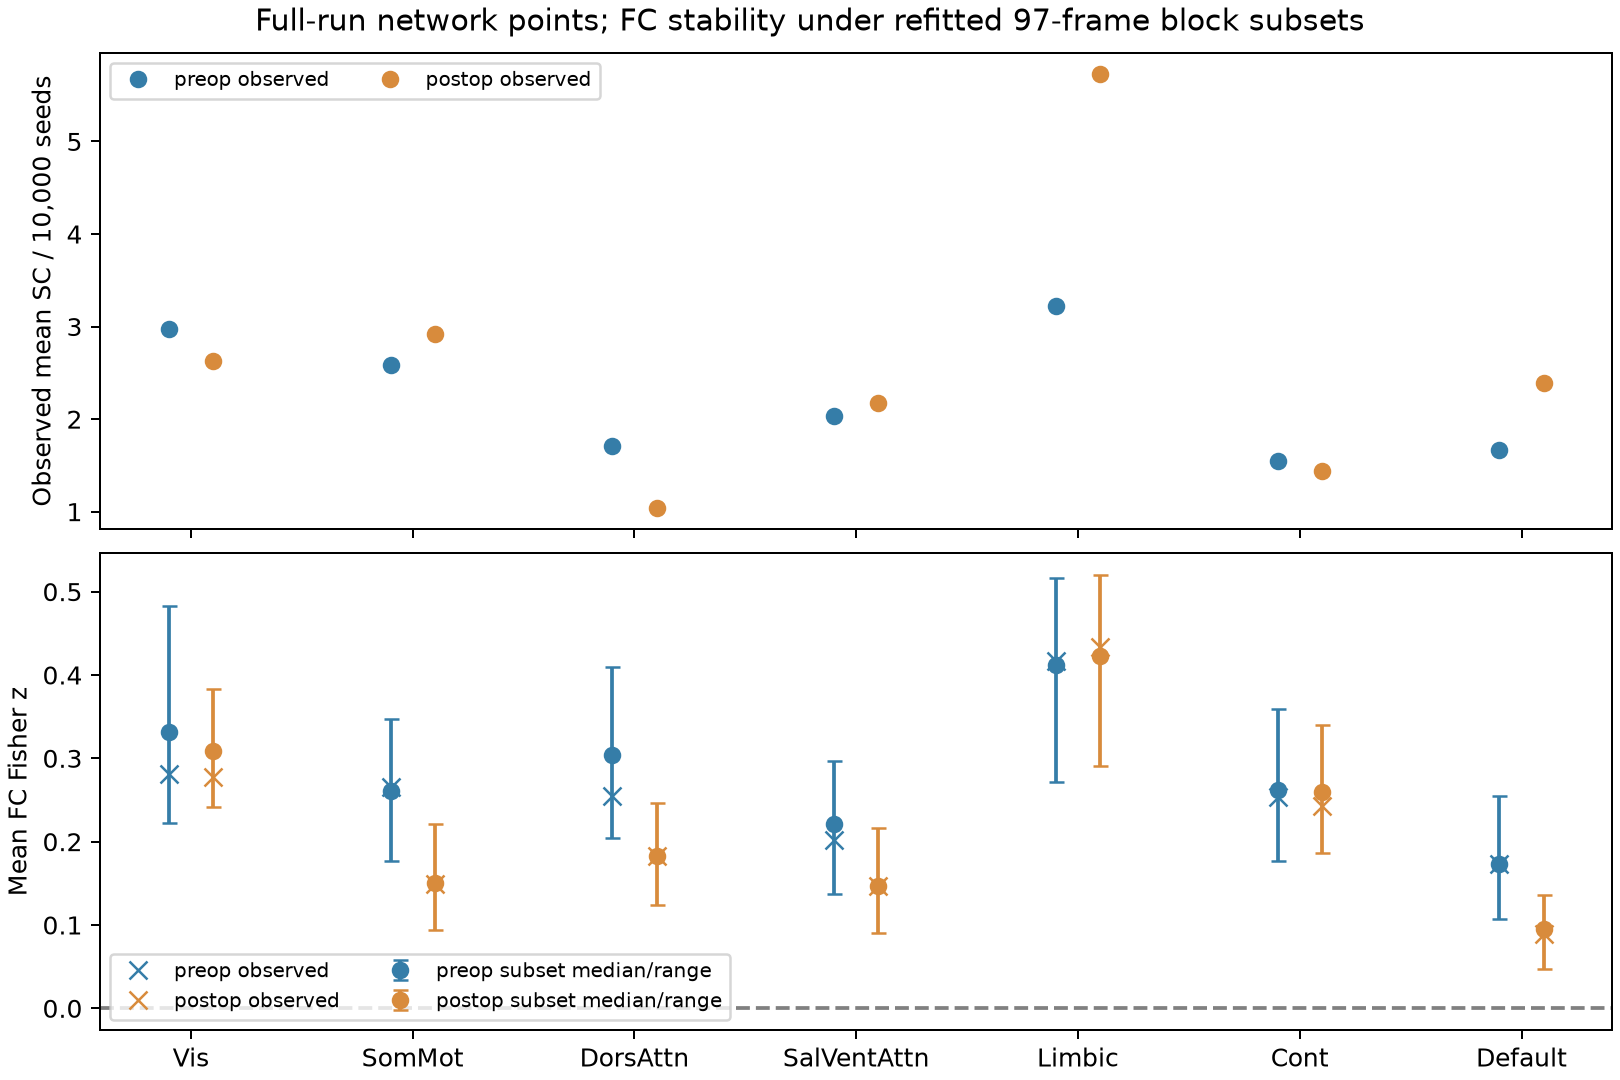
\includegraphics[width=\linewidth]{primary_fc_network_sessions.png}
\caption{Within-network estimates. Crosses mark unchanged observed full-run points. FC circles/ranges summarize the recommended 97-frame fully refitted subsets; SC points use own-consensus seed-rate means. Subset centers do not replace observed FC.}\label{fig:networks}\end{figure}

Mean FC changed from \PreMeanFCPrimary{} to \PostMeanFCPrimary{} in the primary analysis, and from \PreMeanFCStrict{} to \PostMeanFCStrict{} with stricter FD$\leq0.3$ mm censoring. The decrease persists under this censoring sensitivity. GSR gave means near zero (\PreMeanFCGSR{} and \PostMeanFCGSR{}), changing the estimand (Table~\ref{tab:sensitivity}). Strict censoring retains fewer, unequal durations; neither sensitivity is automatically ground truth. Together with the PC-swap result, this prevents interpreting a broad physiological FC decline or a treatment effect. The band-pass preoperative analysis had only 14 residual degrees of freedom and was rejected, preventing a paired band-pass comparison.
\begin{table}[H]\centering\small\begin{tabular}{lrr}
\toprule
Analysis & Mean FC pre $r$ & Mean FC post $r$ \\
\midrule
FD 0.5, high-pass only & 0.0872 & 0.0456 \\
FD 0.3, high-pass only & 0.1085 & 0.0412 \\
FD 1.0, high-pass only & 0.0713 & 0.0541 \\
FD 0.5, whole-brain GSR & 0.0026 & -0.0002 \\
FD 0.5, 0.01--0.1 Hz & -- & 0.0225 \\
\bottomrule
\end{tabular}

\caption{Upper-triangle mean FC sensitivity. A dash denotes QC rejection, not zero FC. All comparisons retain common nodes.}\label{tab:sensitivity}\end{table}

At 2-mm endpoint radius, \PreAssignedTwo{} preoperative and \PostAssignedTwo{} postoperative streamlines were assigned; at 8 mm, yields were \PreAssignedEight{} and \PostAssignedEight{}. These construction sensitivities caution against equating yield with biological damage. Figure~\ref{fig:threshold} shows graph-density sensitivity.
\begin{figure}[H]\centering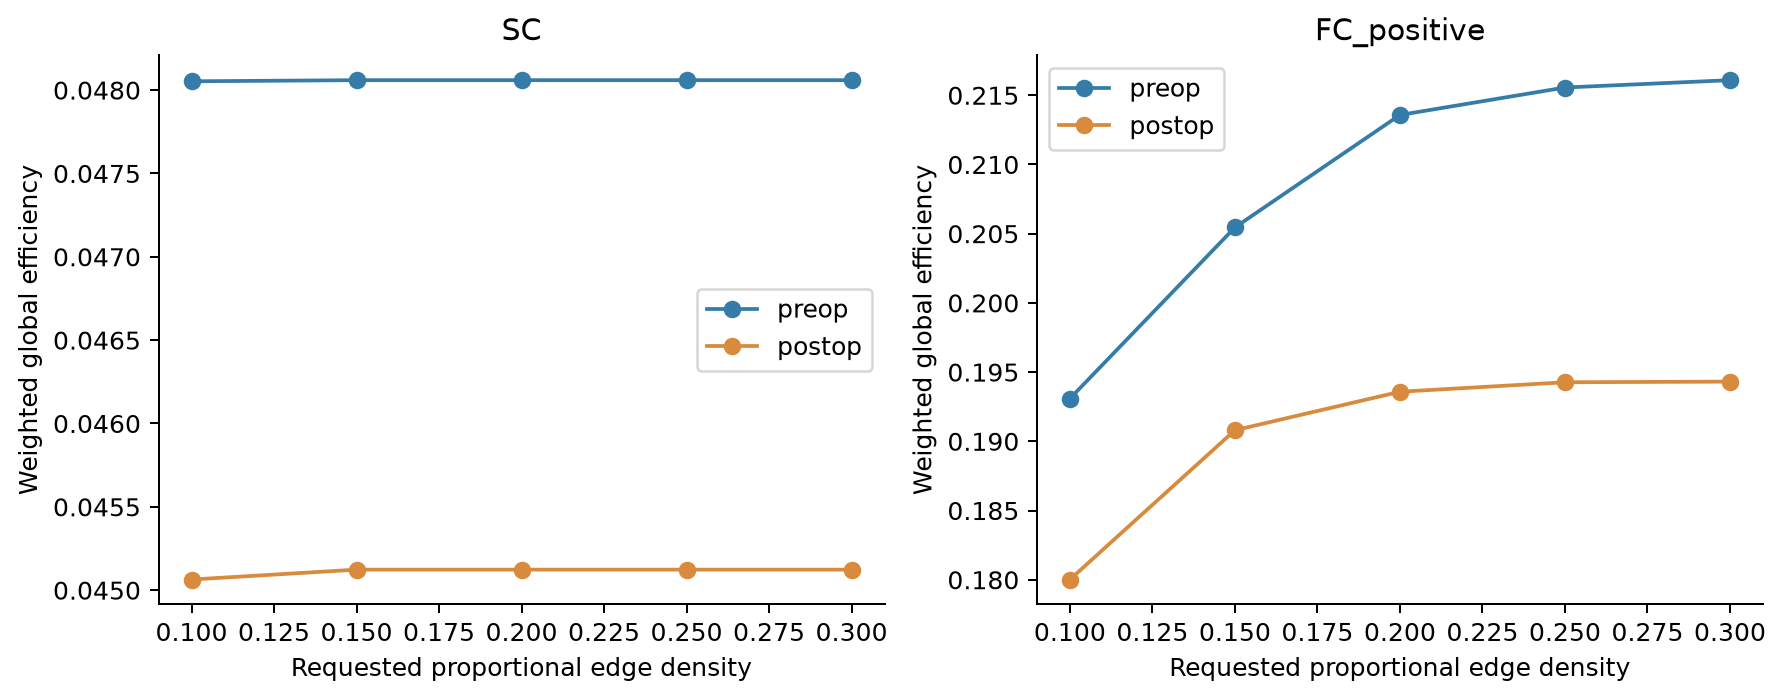
\includegraphics[width=\linewidth]{threshold_sensitivity.png}
\caption{Efficiency versus requested density. Different scales are used for SC and FC; compare sessions within each panel. Own-consensus SC saturates at achieved density 0.2343/0.2349 (1,160/1,163 edges), so requests 0.25/0.30 cannot add edges.}\label{fig:threshold}\end{figure}

\subsection{Mixed cognition and lived experience}
Table~\ref{tab:cognition} and Fig.~\ref{fig:cognition} summarize selected outcomes; Appendix~\ref{app:all} includes all \CantabCount{} CANTAB measures. Simple RT decreased by 58.22 ms (14.4\%), five-choice RT by 34.5 ms (9.5\%), and SSP span rose by one item. MOT latency increased by 26.7 ms (3.3\%) and spatial error by about 0.98 pixels. RVP A-prime was approximately stable, with one postoperative false alarm. SOC minimum-move problems remained 8/12, but four-move problems required more moves and five-move problems fewer. RTI correct counts remained at their source maxima. No change is called statistically significant or reliably changed.
\begin{table}[H]\centering\small\begin{tabular}{lrrr}
\toprule
Measure & Pre-op & Post-op & $\Delta$ \\
\midrule
MOT mean latency (ms) & 817.8 & 844.5 & 26.7 \\
MOT mean spatial error (pixels) & 8.69 & 9.667 & 0.977 \\
RTI simple reaction time (ms) & 403.78 & 345.556 & -58.224 \\
RTI five-choice reaction time (ms) & 361.5 & 327 & -34.5 \\
RVP detection A-prime & 0.95 & 0.952 & 0.002 \\
RVP mean latency (ms) & 448.73 & 455.182 & 6.452 \\
SOC minimum-move problems & 8 & 8 & 0 \\
SOC mean moves: 4-move & 5 & 6.5 & 1.5 \\
SOC mean moves: 5-move & 7.75 & 6.25 & -1.5 \\
SSP span length & 6 & 7 & 1 \\
\bottomrule
\end{tabular}

\caption{Selected raw CANTAB values. $\Delta=\mathrm{post}-\mathrm{pre}$; favorable direction depends on the measure.}\label{tab:cognition}\end{table}
\begin{figure}[H]\centering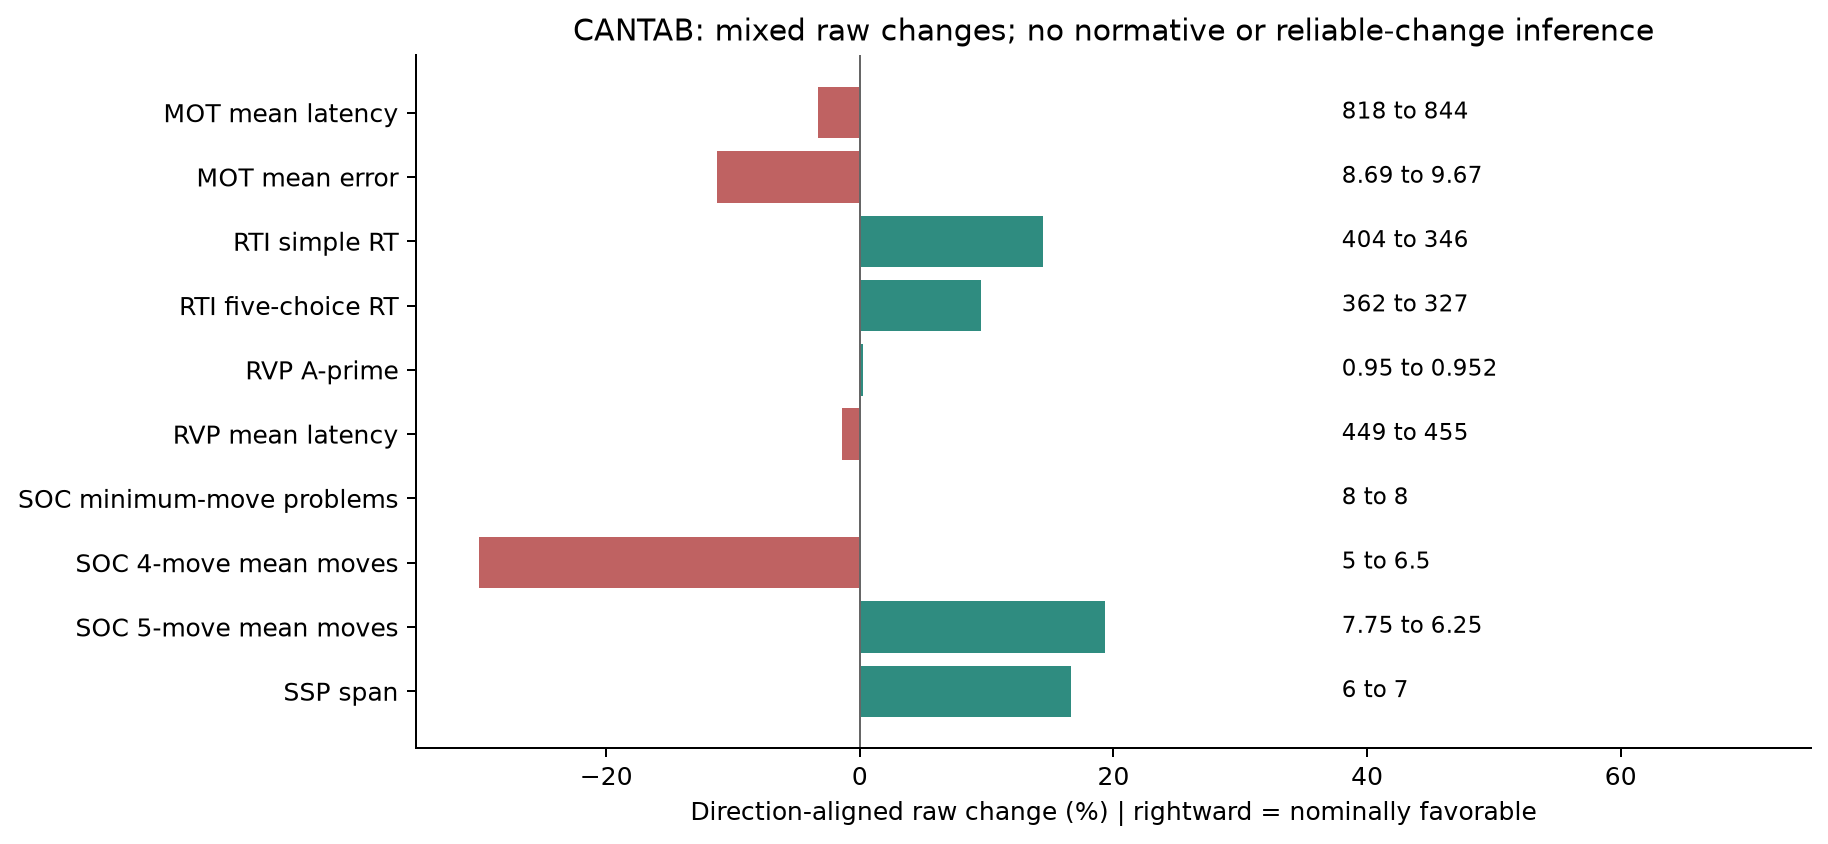
\includegraphics[width=\linewidth]{cognition.png}
\caption{Direction-aligned raw percentages and paired values. Positive direction means nominally favorable, not reliable improvement. Scale differences, ceilings and practice effects prevent treating percentages as commensurate effect sizes.}\label{fig:cognition}\end{figure}

STAI fell from 36 to 30, PSWQ rose from 54 to 61, loneliness rose from 40 to 50, and employment changed from employed to sick leave (Fig.~\ref{fig:psychosocial}). Reappraisal fell from 24 to 14 and suppression rose from 17 to 19, without a universally favorable direction. No dedicated QoL instrument supports a quantified QoL claim.
\begin{figure}[H]\centering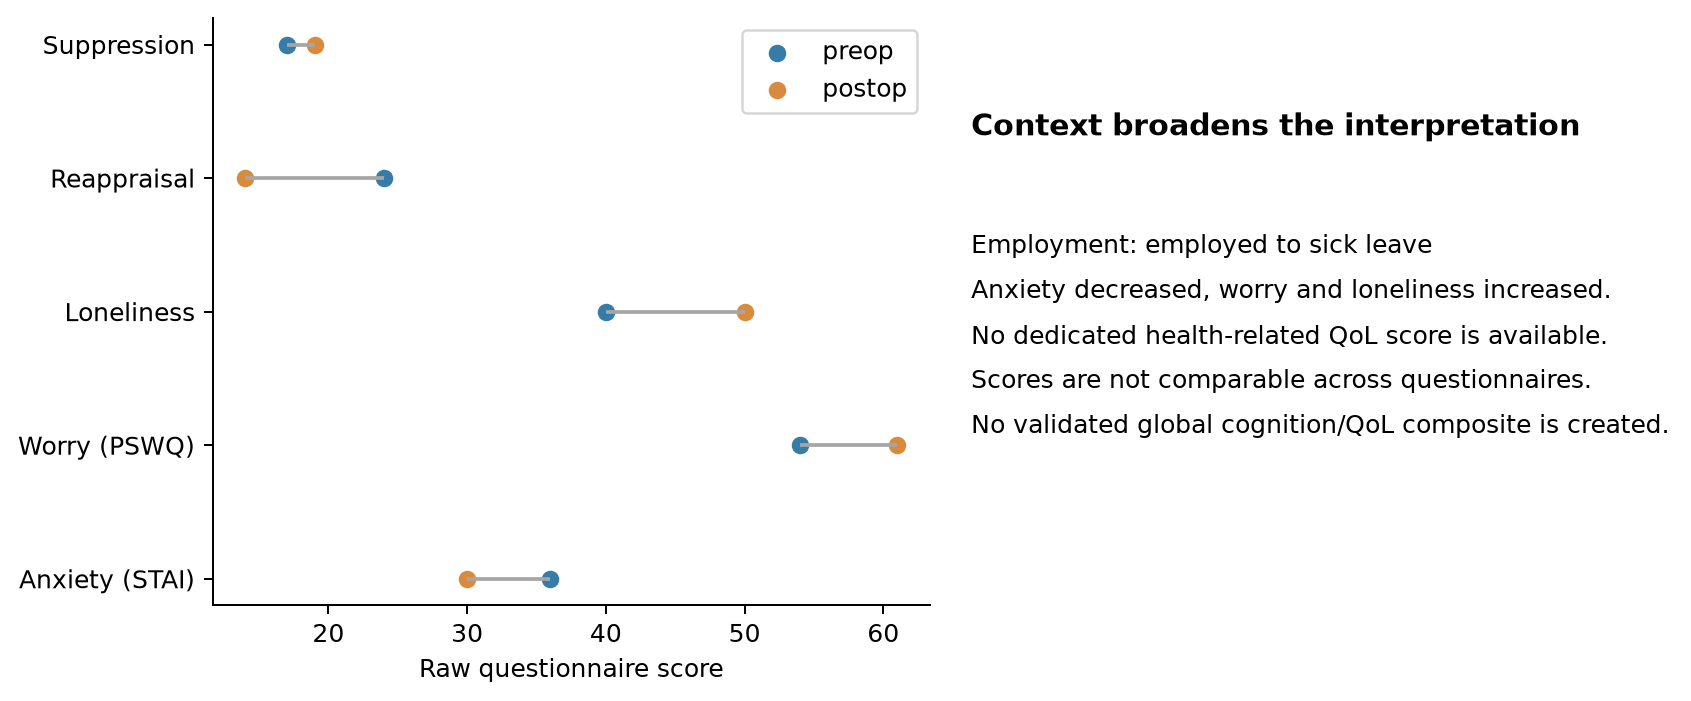
\includegraphics[width=\linewidth]{psychosocial.png}
\caption{Psychosocial raw scores and context. Different instrument scales are not standardized or combined.}\label{fig:psychosocial}\end{figure}

Under the anatomical primary fit, slower motor-screening responses co-occur with lower sensorimotor FC (Fisher $z$, \PreSomMotZ{} to \PostSomMotZ{}). Faster reaction times and longer spatial span also co-occur with lower attention/control FC (control $z$, \PreControlZ{} to \PostControlZ{}). These differing behavioural directions and the nuisance-model dependence preclude interpreting lower FC as uniformly worse cognition. This juxtaposition generates hypotheses without establishing a mechanistic association. Practice, fatigue, vascular changes, motion, treatment, compensation and measurement error cannot be separated by two assessments.

\subsection{Integrating uncertainty with CANTAB and contextual fields}\label{sec:integration}
The assessment profile remains mixed when connectivity uncertainty is made explicit (Table~\ref{tab:evidencetasks}). The primary evidence ledger in \path{results/primary_fc/clinical_evidence_ledger.csv} covers all 28 CANTAB and 19 psychosocial/context fields; Appendices~\ref{app:cantab} and~\ref{app:psych} retain the complete source values and field dictionaries. Notebook 12 lets the reader select each field and inspect candidate network evidence with its original units, caveats and missingness. Clinical changes have no estimated measurement-error interval in these data.
The recommended subset ranges now provide the main FC stability layer (Table~\ref{tab:primaryfcnetworks}; Fig.~\ref{fig:primaryfcnetworks}). Sensorimotor observed $\Delta z=-0.1158$ has median $-0.1093$ and range $[-0.2064,-0.0170]$; this coexists with slower MOT and faster RTI, with different task demands. The earlier matched-count block range crossed zero, so the negative primary range is design-conditional and cannot diagnose a motor deficit. Dorsal-attention range is $[-0.2393,-0.0050]$, while control $[-0.1312,+0.1283]$ spans zero despite faster RTI and longer SSP. Mixed SOC difficulty effects and stable RVP A-prime remain separate measurements. Visual median is $-0.0209$ with range $[-0.1594,+0.1081]$, close to the unchanged observed $-0.0045$ compared with the earlier repeated-row median $-0.1993$. Default-network range now crosses zero, $[-0.1649,+0.0058]$, although some preceding bootstrap/subset designs were negative. These changes reinforce dependence on the sampling design, not evidence of compensation, recovery or a cognitive mechanism.
\begin{table}[H]\centering\scriptsize\setlength{\tabcolsep}{3pt}\begin{tabular}{lrrrrr}
\toprule
Network & SC $\Delta$ & SC range & FC $\Delta z$ & FC median & FC range \\
\midrule
Vis & -0.343 & [-0.385, -0.308] & -0.004 & -0.021 & [-0.159, +0.108] \\
SomMot & +0.336 & [+0.283, +0.371] & -0.116 & -0.109 & [-0.206, -0.017] \\
DorsAttn & -0.665 & [-0.712, -0.624] & -0.071 & -0.123 & [-0.239, -0.005] \\
SalVentAttn & +0.138 & [+0.082, +0.187] & -0.055 & -0.074 & [-0.167, +0.032] \\
Limbic & +2.507 & [+2.279, +2.662] & +0.017 & +0.010 & [-0.149, +0.180] \\
Cont & -0.115 & [-0.159, -0.076] & -0.010 & -0.001 & [-0.131, +0.128] \\
Default & +0.728 & [+0.707, +0.748] & -0.083 & -0.081 & [-0.165, +0.006] \\
\bottomrule
\end{tabular}

\caption{Primary within-network evidence. SC uses own-support reselection in the 500 whole-run bootstraps; FC uses 200 fully refitted 97-frame subsets. Observed changes and distribution medians are separate; all ranges are raw conditional percentiles. Units differ between modalities.}\label{tab:primaryfcnetworks}\end{table}
\begin{figure}[H]\centering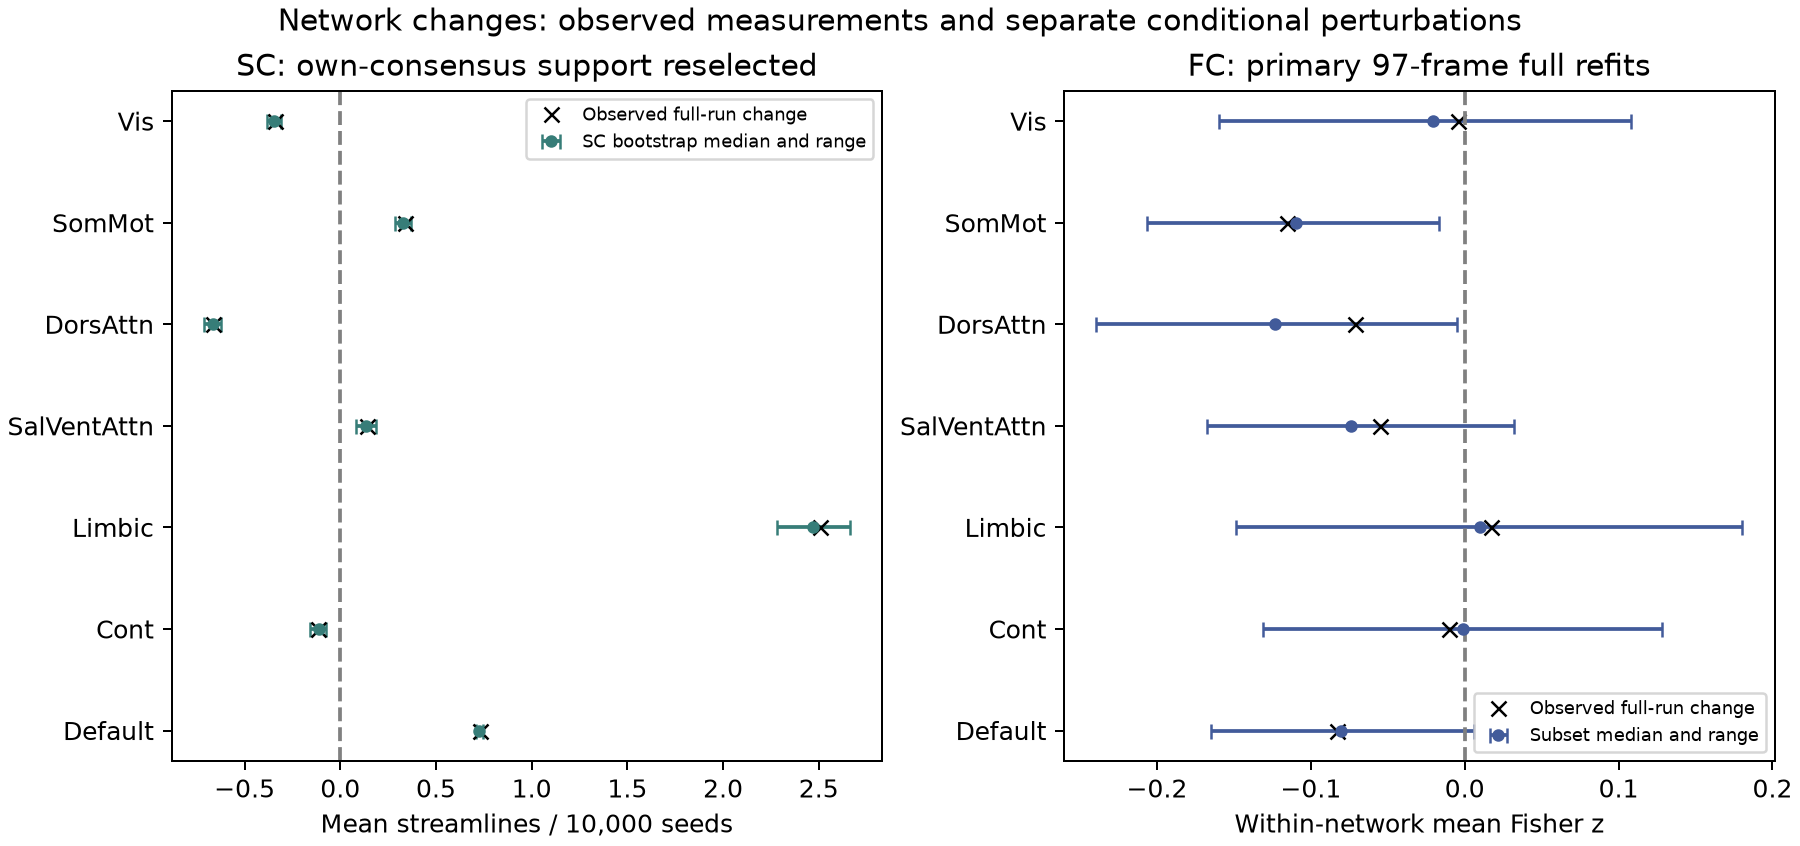
\includegraphics[width=\linewidth]{primary_fc_network_changes.png}
\caption{Primary conditional network evidence with unchanged observed crosses. Seven dependent exploratory summaries are not multiplicity-corrected tests or clinical reliable-change intervals. The complete 47-field ledger retains all assessment values and missingness.}\label{fig:primaryfcnetworks}\end{figure}

\textbf{Retained sensitivity evidence.} The following frozen/refitted bootstrap and previous block-subsampling tables and figure preserve the preceding investigation. Their different targets explain why individual ranges differ from the recommended primary ranges; they are not interchangeable clinical error bars.
\begin{table}[H]\centering\footnotesize\begin{tabular}{lp{.45\linewidth}p{.30\linewidth}}
\toprule
Evidence & Observed profile & Candidate networks (hypotheses) \\
\midrule
MOT & Latency +26.7 ms; spatial error +0.977 pixels & SomMot; Vis \\
RTI & Simple RT -58.22 ms; correct counts unchanged & DorsAttn; SalVentAttn; SomMot \\
RVP & A-prime +0.00236; false alarms 0 to 1 & DorsAttn; SalVentAttn; Cont \\
SOC & Minimum-move problems 8/12; 4/5-move changes differ & Cont; DorsAttn \\
SSP & Span 6 to 7 & DorsAttn; Cont; Vis \\
Context & STAI -6; PSWQ +7; loneliness +10; sick leave & No network assigned \\
\bottomrule
\end{tabular}

\caption{Descriptive task/context alignment. Network lists are broad didactic hypotheses, not validated patient-specific mappings. Signs retain raw units; RT means reaction time. All source fields, including task subtleties and ambiguous codes, remain in the appendices and evidence ledger.}\label{tab:evidencetasks}\end{table}
\begin{table}[H]\centering\scriptsize\setlength{\tabcolsep}{3pt}\begin{tabular}{lrrrrr}
\toprule
Network & SC $\Delta$ & SC range & FC $\Delta z$ & FC frozen range & FC refit range \\
\midrule
Vis & -0.343 & [-0.385, -0.308] & -0.004 & [-0.092, +0.072] & [-0.437, +0.076] \\
SomMot & +0.336 & [+0.283, +0.371] & -0.116 & [-0.210, -0.041] & [-0.430, -0.024] \\
DorsAttn & -0.665 & [-0.712, -0.624] & -0.071 & [-0.143, +0.013] & [-0.415, +0.010] \\
SalVentAttn & +0.138 & [+0.082, +0.187] & -0.055 & [-0.118, +0.006] & [-0.308, +0.026] \\
Limbic & +2.507 & [+2.279, +2.662] & +0.017 & [-0.118, +0.156] & [-0.248, +0.233] \\
Cont & -0.115 & [-0.159, -0.076] & -0.010 & [-0.099, +0.079] & [-0.228, +0.133] \\
Default & +0.728 & [+0.707, +0.748] & -0.083 & [-0.143, -0.037] & [-0.329, -0.010] \\
\bottomrule
\end{tabular}

\caption{Within-network observed changes and conditional 2.5/97.5 percentiles. SC units are mean streamlines per 10,000 attempted seeds over all within-network pairs; support is reselected in each SC bootstrap. FC units are mean Fisher $z$ over the same anatomical pairs, using the historical repeated-row ten-frame bootstrap draws with frozen/full nuisance training. SC and FC ranges have separate perturbation sources and units.}\label{tab:evidencenetworks}\end{table}
\begin{figure}[H]\centering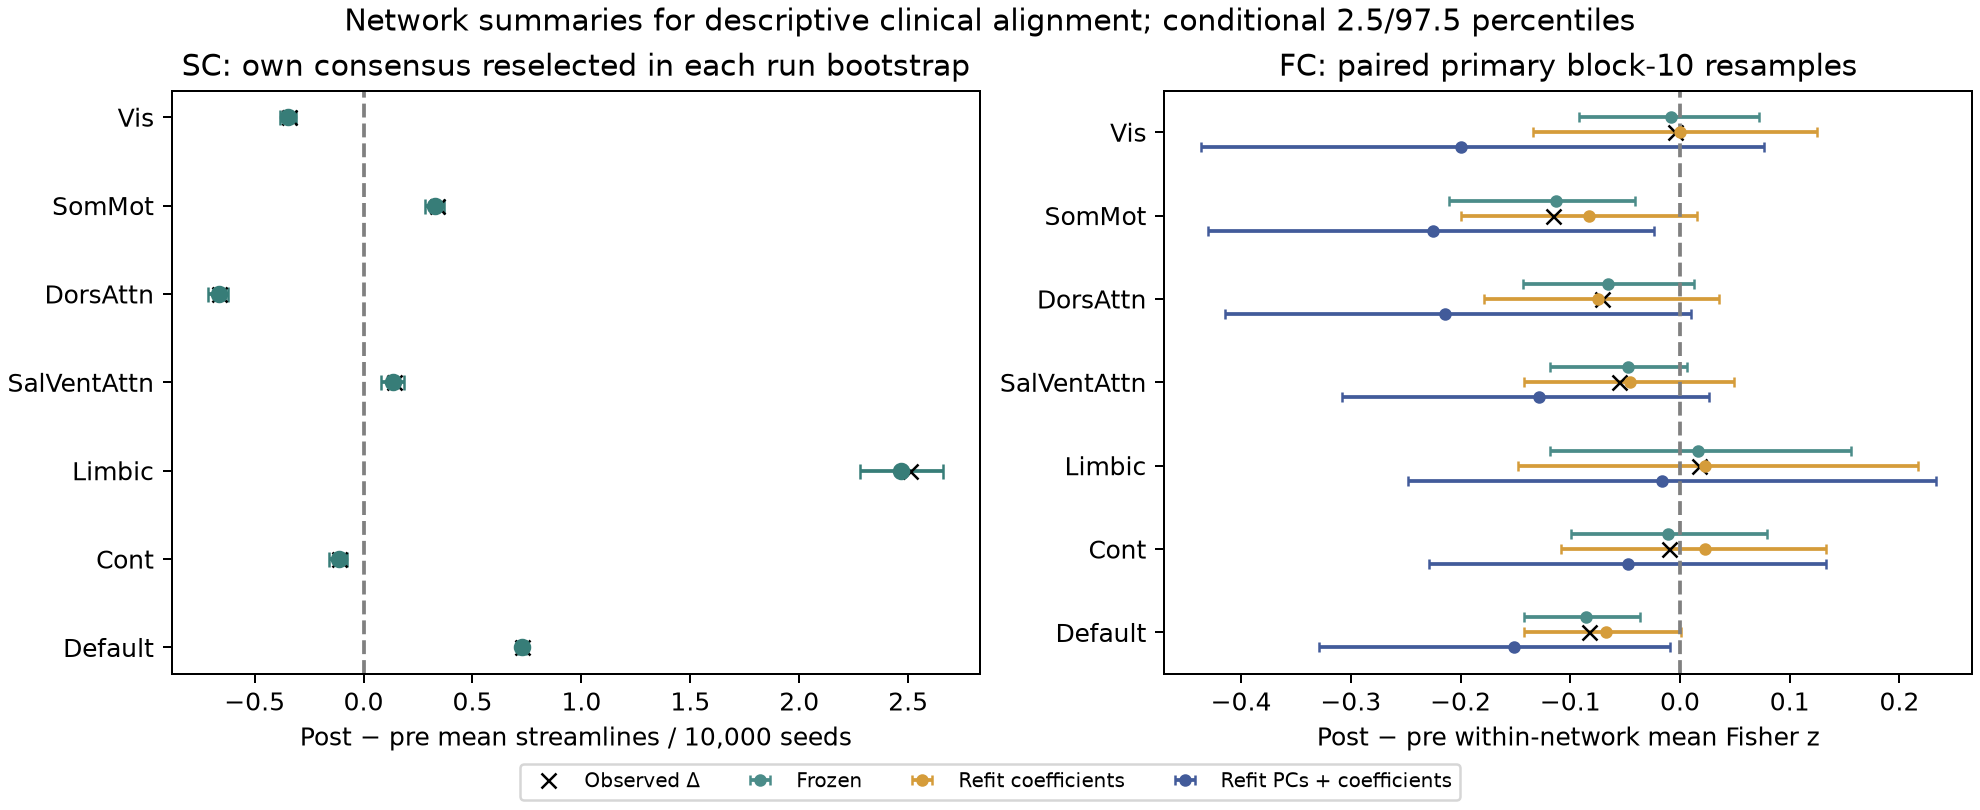
\includegraphics[width=\linewidth]{evidence_network_uncertainty.png}
\caption{Measured network changes (crosses) alongside conditional sampling distributions. Bootstrap centers can differ substantially from observed changes after PC retraining; they are not corrected measurements. The panels are not a cognitive or QoL prediction.}\label{fig:evidencenetworks}\end{figure}

Sensorimotor observed FC changes by $-0.1158$ Fisher $z$; its fully refitted range is $[-0.4298,-0.0238]$, versus frozen $[-0.2105,-0.0410]$. This co-occurs with slower MOT but faster RTI, which both involve motor responses and differing task demands. Its SC network mean increases by $+0.3363$ per 10,000 seeds, while dorsal-attention SC decreases by $-0.6654$. Such dissociation is compatible with multiple measurement/model contributions and cannot establish damage or compensation. Control-network FC changes by only $-0.0101$, with a full-refit range $[-0.2284,+0.1334]$; faster RTI, SSP span 6 to 7 and difficulty-dependent SOC changes cannot establish preserved or improved executive circuitry. Dorsal-attention and visual FC refit ranges also cross zero. Default-network FC has a negative full-refit central range, but these seven exploratory network summaries are neither corrected hypothesis tests nor clinical associations.

Retrained FC ranges can be markedly displaced: visual-network median change is $-0.1993$ after full refitting versus the observed $-0.0045$. This reflects the nonlinear, short-sample training estimator under repeated rows, not a revised clinical estimate or evidence of a visual deficit. The fact that global coupling and within-network mean FC can move differently follows from their different statistics and edge populations. We retain the observed values and all three model distributions explicitly rather than using bootstrap medians as replacement outcomes.

\textbf{Clinical interpretation after sampling-design controls.} Table~\ref{tab:pcnetworkcenters} and Figure~\ref{fig:pcnetworks} show that visual-network median change moves from $-0.1993$ with the bootstrap to $-0.0458$ at unit coverage, $-0.0355$ with independently sampled matched-count blocks and $-0.0143$ at 80\% retention; the observed $-0.0045$ is unchanged. This weakens any interpretation of the large bootstrap displacement as a measured visual deficit. For sensorimotor FC, the matched-count block range is $[-0.2234,+0.0246]$, crossing zero, whereas the earlier full-refit bootstrap range is negative. Its observed $-0.1158$ and the measured coexistence of slower MOT and faster RTI remain unchanged. There is no stable network-to-task explanation established by these intervals.

Dorsal-attention ranges become negative in the new block-10 subsets, despite crossing zero in the bootstrap; default-network ranges remain negative. These seven dependent, exploratory summaries are not corrected tests, reliable-change intervals or individual localization. Control-network intervals span zero across designs, while SSP span increases and SOC difficulty levels change differently. The comparison reinforces a mixed assessment profile with unresolved brain--behaviour mechanisms. It neither establishes compensation nor links a chosen connectivity sign to anxiety, worry, loneliness or sick leave. The 80\% intervals reflect conditional subset variability and cannot validate cognitive or QoL decline. Appendices and all 47 clinical source fields remain unchanged; notebook 12 adds field-specific comparisons of these network ranges.
\begin{table}[H]\centering\small\begin{tabular}{lrrrrr}
\toprule
Network & Observed & Bootstrap & Unit weights & Blocks, matched & Blocks, 80\% \\
\midrule
Vis & -0.0045 & -0.1993 & -0.0458 & -0.0355 & -0.0143 \\
SomMot & -0.1158 & -0.2252 & -0.1148 & -0.1125 & -0.1062 \\
DorsAttn & -0.0713 & -0.2145 & -0.1256 & -0.1203 & -0.0920 \\
SalVentAttn & -0.0553 & -0.1286 & -0.0700 & -0.0723 & -0.0569 \\
Limbic & +0.0173 & -0.0166 & +0.0075 & -0.0090 & +0.0239 \\
Cont & -0.0101 & -0.0470 & -0.0091 & -0.0150 & +0.0017 \\
Default & -0.0832 & -0.1514 & -0.0907 & -0.0888 & -0.0824 \\
\bottomrule
\end{tabular}

\caption{Observed within-network FC changes and full-refit distribution medians, ten-frame designs, Fisher $z$. Centers describe resampled estimators and never replace observed changes. ``Unit weights'' retains the exact bootstrap coverage; ``matched'' uses independent nonoverlapping blocks at identical distinct counts.}\label{tab:pcnetworkcenters}\end{table}
\begin{table}[H]\centering\scriptsize\setlength{\tabcolsep}{3pt}\begin{tabular}{lrrrr}
\toprule
Network & Bootstrap & Unit weights & Blocks, matched & Blocks, 80\% \\
\midrule
Vis & [-0.437, +0.076] & [-0.214, +0.099] & [-0.239, +0.127] & [-0.160, +0.082] \\
SomMot & [-0.430, -0.024] & [-0.237, -0.002] & [-0.223, +0.025] & [-0.170, -0.032] \\
DorsAttn & [-0.415, +0.010] & [-0.278, -0.016] & [-0.249, -0.015] & [-0.193, -0.008] \\
SalVentAttn & [-0.308, +0.026] & [-0.179, +0.027] & [-0.181, +0.023] & [-0.116, +0.005] \\
Limbic & [-0.248, +0.233] & [-0.179, +0.183] & [-0.197, +0.197] & [-0.103, +0.132] \\
Cont & [-0.228, +0.133] & [-0.154, +0.121] & [-0.131, +0.122] & [-0.083, +0.095] \\
Default & [-0.329, -0.010] & [-0.191, -0.017] & [-0.204, -0.004] & [-0.139, -0.030] \\
\bottomrule
\end{tabular}

\caption{Central 2.5/97.5 percentiles accompanying Table~\ref{tab:pcnetworkcenters}. All 200 FC draws are retained. Within-network FC uses all anatomical pairs; these are different edge populations and statistics from SC--FC coupling.}\label{tab:pcnetworkranges}\end{table}
\begin{figure}[H]\centering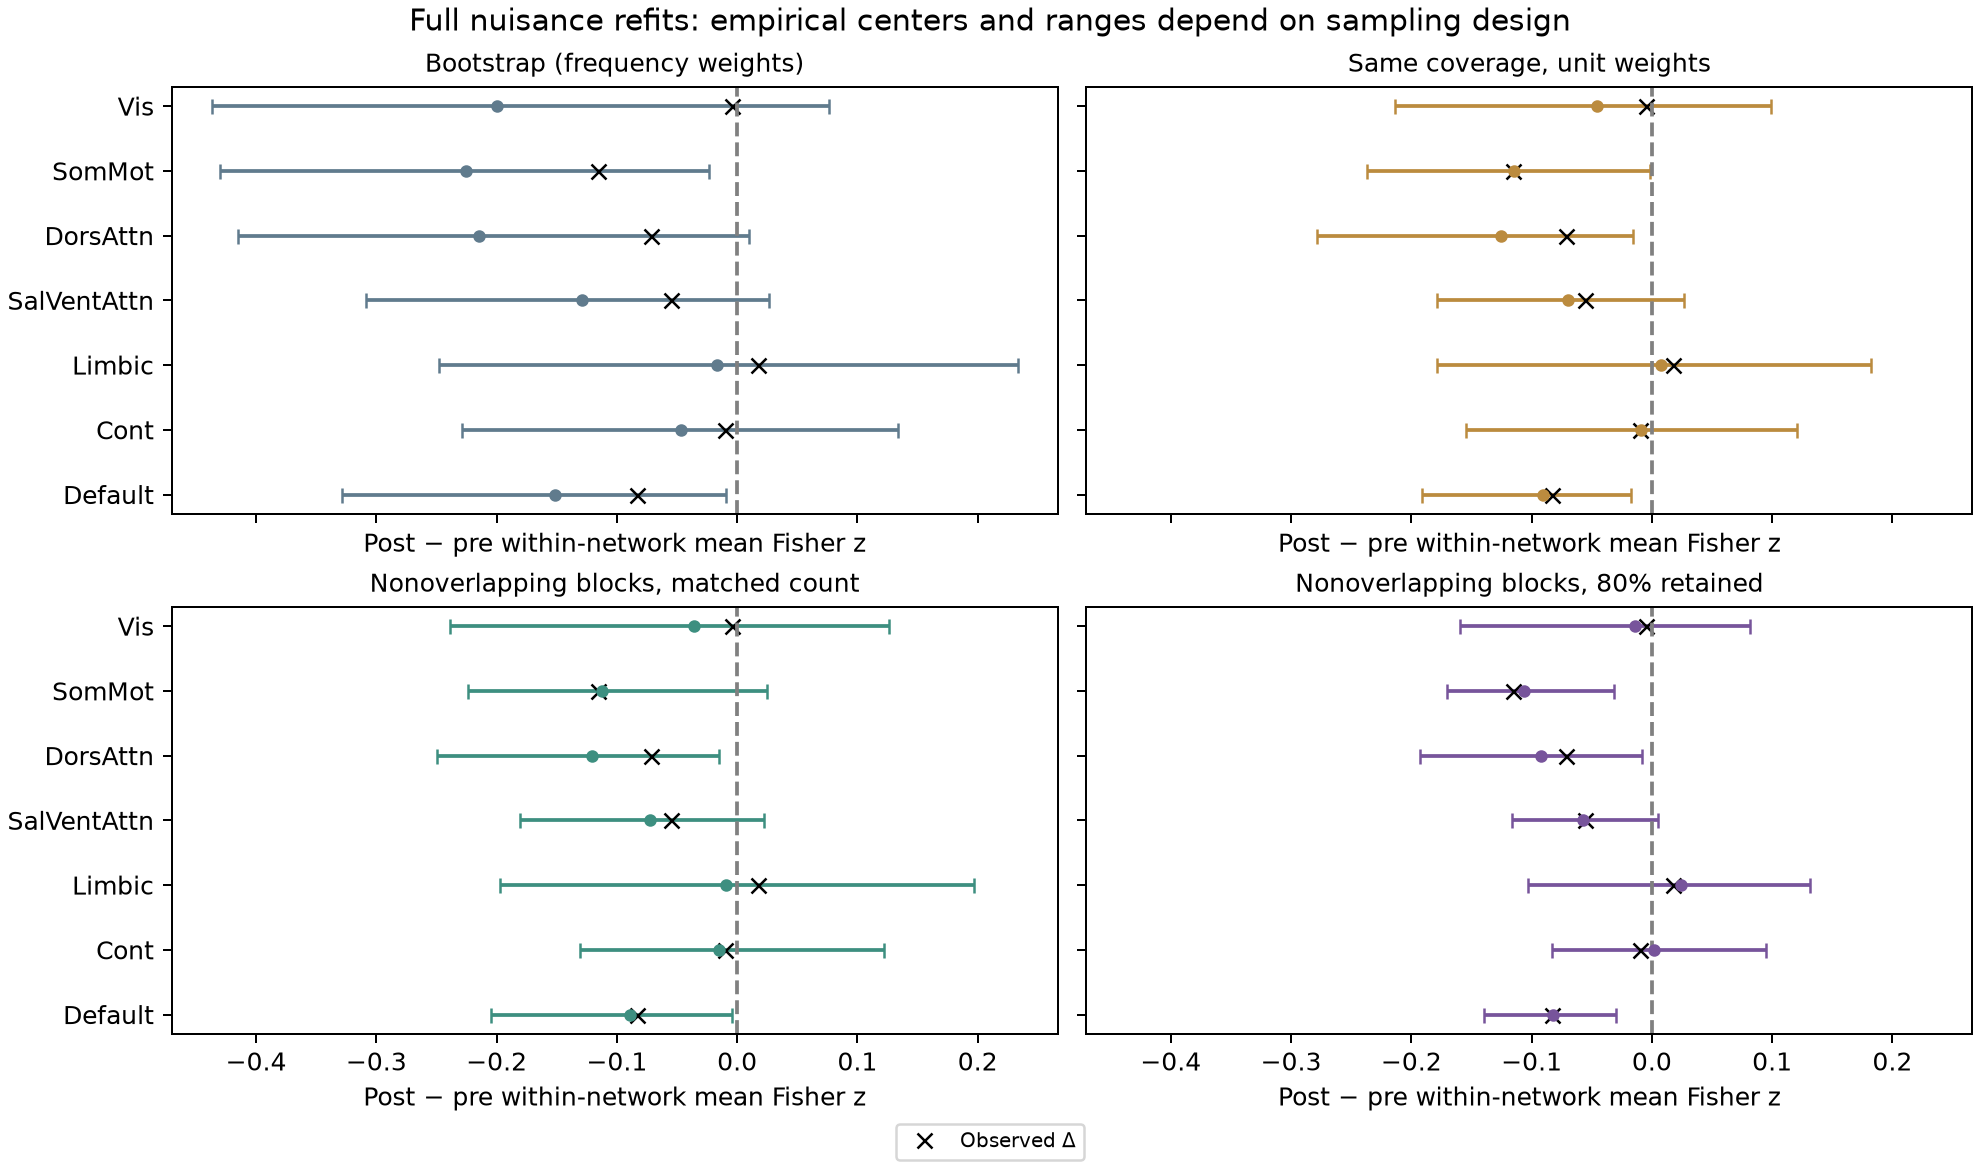
\includegraphics[width=\linewidth]{pc_sampling_networks.png}
\caption{Network FC distributions change with weighting, coverage and retained fraction. Black crosses are the unchanged observed changes. No clinical error bars, latent cognitive score or network--QoL prediction is inferred.}\label{fig:pcnetworks}\end{figure}

STAI $36\rightarrow30$, PSWQ $54\rightarrow61$, loneliness $40\rightarrow50$, reappraisal $24\rightarrow14$, suppression $17\rightarrow19$ and employed $\rightarrow$ sick leave describe different emotional, regulatory and participation dimensions. They are unlocalized contextual evidence, not nuisance covariates fitted from two sessions. ERQ processing/expression remain undocumented scales; education remains an unlabelled code. Pre-only lifestyle frequencies/indices remain missing post-op, while post-only ``Same''/``Less'' responses remain relative categories. None is imputed or collapsed into a QoL score. Without dated assessments, treatment/medication information, fatigue/sleep context, retest norms, repeat imaging and a dedicated QoL instrument, this integration supports targeted questions for future measurement, not a mechanism linking surgery, connectivity and wellbeing.

\section{Didactic simulations}
All injury severity, growth and dynamical predictions are simulated; baseline anatomy and reconstructed own-consensus repeat-mean SC come from patient data. The simulations are regenerated under the primary policy; earlier single-run simulations are archived. A graph Fisher--KPP analogue is
\begin{equation}\dot{\boldsymbol c}=-D L\boldsymbol c+\rho\boldsymbol c\odot(1-\boldsymbol c),\end{equation}
with SC Laplacian $L$. The exported 100-step forward-Euler simulation uses $\Delta t=0.2$ arbitrary units, $D=0.5$, $\rho=0.3$, concentration clipping to $[0,1]$, and the maximal lesion-overlap parcel as its seed. No growth parameter is fitted, and graph transport is not asserted to model glioma infiltration.

A hypothetical injury defines $e_i=\exp(-d_i/10\,\mathrm{mm})$, where $d_i$ is minimum parcel-to-lesion distance, and attenuates edges:
\begin{equation}W'_{ij}=(1-se_i)W_{ij}(1-se_j),\quad 0\leq s\leq1.\end{equation}
This endpoint rule is not a reconstructed resection or measured tract injury. The baseline weight scale stays fixed.

An Ornstein--Uhlenbeck model uses $d\boldsymbol x=A\boldsymbol x\,dt+d\boldsymbol B$, with $A=-I+gW'/\lambda_{\max}(W_{pre})$ and $0\leq g<1$. Stationary covariance solves $A\Sigma+\Sigma A^T+I=0$; normalized covariance is model FC. The exported sweep fixes $g=0.6$. Symmetric positive SC and linear dynamics cannot reproduce all signed empirical FC; the model omits BOLD haemodynamics, delays, inhibition and plasticity. Figure~\ref{fig:sim} illustrates mechanisms without predicting cognition or selecting a surgical plan.
\begin{figure}[H]\centering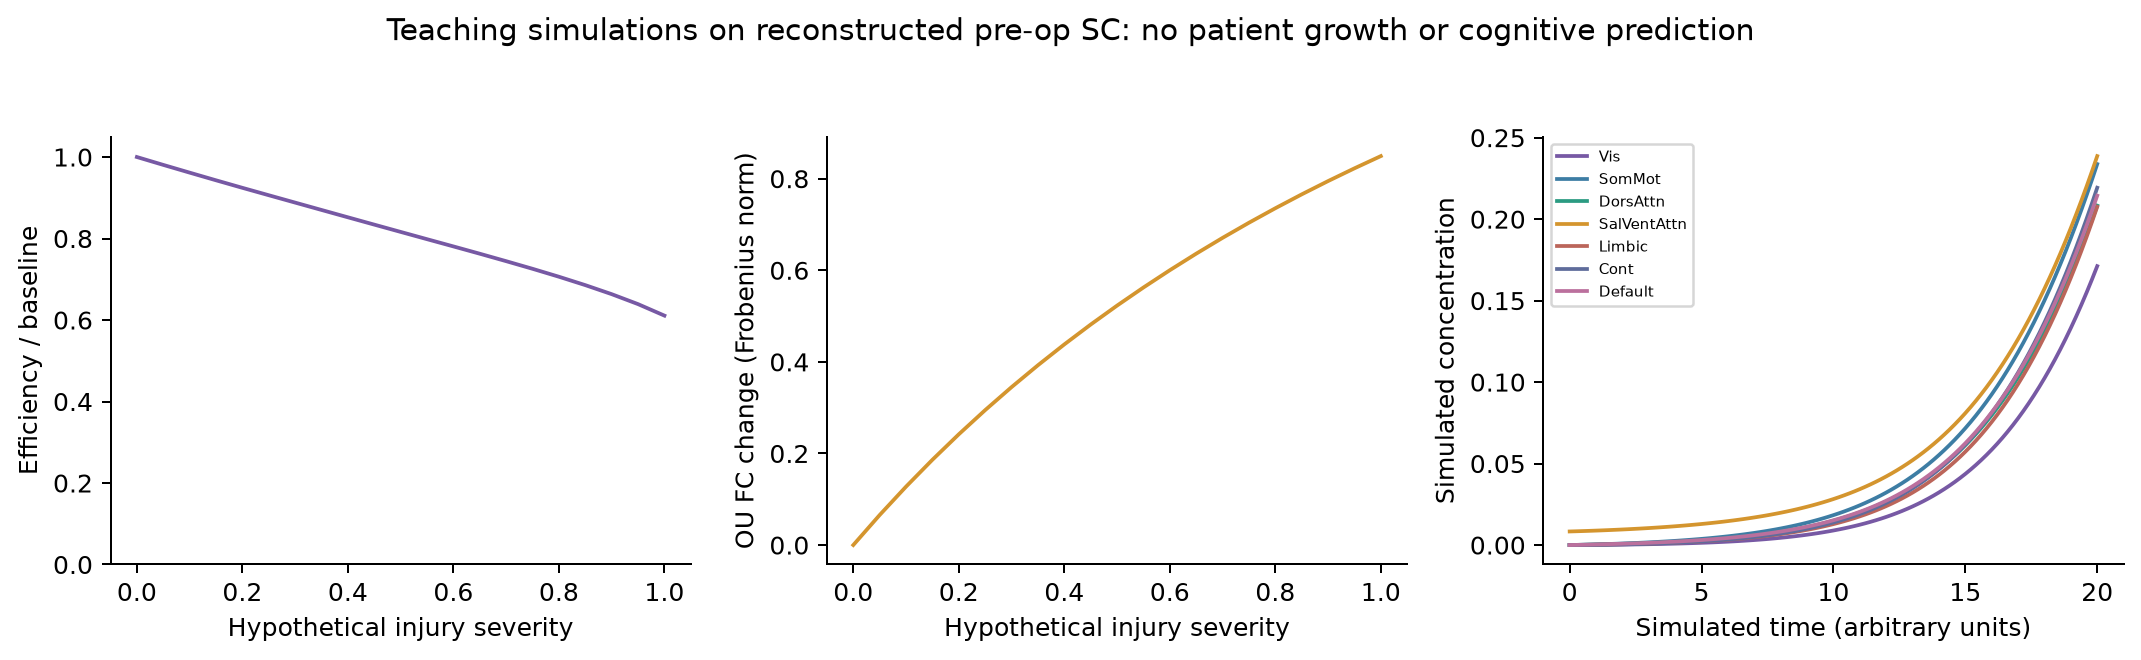
\includegraphics[width=\linewidth]{simulations.png}
\caption{Teaching scenarios: injury attenuation, OU FC and graph reaction--diffusion on reconstructed baseline SC. Concentration, severity, model FC and time are simulated.}\label{fig:sim}\end{figure}

\section{Discussion and limitations}
The contribution is an auditable bridge between anatomy, networks and multidimensional outcomes. It reconstructs actual paired connectomes and retains all assessments rather than reducing the subject to lesion volume or one cognitive score. A central result is analytical fragility: FC magnitude, nuisance dependence and reconstructed SC depend on processing choices. These sensitivities deserve prominence over a selected biological narrative.

The revised workflow combines Python reconstruction with FSL topup/eddy. An earlier version incorrectly described the multi-shell acquisition as single-shell and fit CSD across shells; its outputs are archived and superseded. The new rigid-only comparator uses the same revised shell selection as corrected data, so the matched comparison assesses the preprocessing package and its downstream registration rather than conflating it with this model correction. Neither comparison is a ground-truth validation. Nonpositive AP or PA Jacobians are excluded from the tensor/CSD brain mask. The fitted susceptibility field can be uncertain where signal is lost, and eddy's replacement of slices is model based.

The BOLD revision makes susceptibility correction explicit, but field transfer relies on unavailable shim compatibility and inconsistent timing metadata. Similarity across two displacement amplitudes does not test these assumptions. The new investigation identifies a resampling/mask/cutoff interaction. T1-based WM/CSF models reduce the old/new processing gap but remove substantial shared cortical variance; physiological recordings and independent segmentation review remain necessary to assess signal specificity. The recommended anatomical five-PC model is a fixed, post hoc methodological choice across both sessions. Anatomical specificity and retained-frame training justify its priority, while the full alternative-model results constrain interpretation. A favourable cognitive narrative must not determine denoising choices. Slice timing and motion-dependent susceptibility remain unmodelled.

The historical single-run strict-censoring reversal is a computational interaction: restricting frames alone does not reverse coupling, whereas refitting the small-sample regression/PCA can do so. Duration/FD matching does not settle the sign, and coarse time matching changes it again. Shared-support and fixed-reference SC controls further alter the contrast. The edge/network analysis (Section~\ref{sec:edgeresults}) identifies pre-op-only edges as the largest original signed term, but reranked deletions and matched replay give different localizations. Global rank context and substantial cancellation preclude a unique biological edge or network explanation. These results support reporting methodological uncertainty rather than a single directional brain--behaviour account. Equal frame count and FD do not equate serial dependence, physiology, neural states or repeated-scan reliability. Longer repeat acquisitions and independent motion/physiological QC would be needed to distinguish those mechanisms.\par

The primary common-consensus reference yields negative primary/strict point contrasts. Joint sampling (Section~\ref{sec:jointresults}) shows much larger FC than 20-run seed-mean variability at fixed support, while support reselection adds rank-population sensitivity. Full-run block ranges cross zero; the negative strict FD-matched central range changes after run-half matching. The frozen branch is retained as a sensitivity; the preceding full-run bootstrap refits all nuisance training (Section~\ref{sec:refitresults}). Its central range is wider and shifted toward zero, while strict full-run refits fail the explicit distinct-frame guard. Matched short-subset refits remain complementary controls. The new factorial and block-subsampling controls (Section~\ref{sec:pcsamplingresults}) show that repeated-row weighting changes the learned nuisance space and shared-signal removal, especially preoperatively. This explains much of the empirical recentering without identifying population bias or signal specificity. Unit-coverage and matched-count block ranges cross zero; the narrower negative 80\% ranges are retained-fraction sensitivities, not evidence overturning the unresolved biological direction. These conditional ranges leave acquisition, model and clinical measurement uncertainty unestimated. Acquisition/model uncertainty and reliable biological direction remain unresolved. Its methodological justification is repeated occurrence and fixed edge population, not the negative sign. Repeated tracking (Section~\ref{sec:screliabilityresults}) addresses conditional seed-sampling variability: many original session-specific edges reappear in the opposite scan and singleton occurrence is substantially lower than high-count occurrence. However, consensus can reproduce systematic false pathways, while count cutoffs alter the ranked edge population rather than selectively removing demonstrated errors. The seed, count, consensus and matched-FC controls together strengthen the conclusion of methodological sensitivity; they do not validate a new surgical disconnection map or resolve the coupling direction.

Affine atlas mapping and rigid longitudinal transport cannot fully handle resection-related deformation. Lesion-aware nonlinear/surface registration, validated nuisance tissue masks, acquisition/model uncertainty, justified tract weights such as ACT/SIFT2 and independent expert QC should precede stronger claims. Endpoint-radius sensitivity does not capture total tractography uncertainty.

Cortical-only analysis omits subcortical, cerebellar and brainstem pathways. Resting FC reflects vascular as well as neural physiology; lower FC or higher efficiency is not universally better. Atlas network identities may be displaced or reorganized. Clinical interpretation requires timing, medications/treatment, norms, reliability and matched retest data. A dedicated QoL scale would measure a distinct outcome, not be inferred from anxiety or sick leave. Network--cognition models need prespecified hypotheses and cohort-level out-of-sample validation. This case supports methodological exploration, not treatment guidance or validation of a predictive twin.

The recommended FC stability target is equal-duration, nonreplacement, fully refitted subsets (Section~\ref{sec:primaryfcmethods}), with observed points kept distinct from conditional subset distributions. Its primary coupling range crosses zero; network signs vary with fraction and training. A fixed fraction, small residual sample and post hoc selection prevent calibrated biological or clinical inference. Freezing fits understates training sensitivity, while repeated-row retraining changes the empirical PCA problem. Neither a desired coupling sign nor agreement with a task should select among these methods.

\section{Reproducibility and educational use}
The separate folder contains raw PAT16 inputs and sidecars, original derivatives, atlas/templates, SHA256 manifest, exact \texttt{uv.lock}, Python source, fifteen notebooks, matrices, transforms, tables, figures, simulations and this LaTeX/BibTeX project. Runtime code does not depend on the sibling repository. The public source repository is \url{https://github.com/arvidl/glioma-connectivity-and-cognition}. Source, executed notebooks, generated report figures/tables and \path{report/main.pdf} are tracked by ordinary Git. Larger inputs and analysis checkpoints are distributed as seven checksummed multipart assets (about 4.9 GiB) in release \texttt{v0.1.0-assets}. The committed \path{reproducibility/assets.json} records public URLs, sizes and SHA256 values for every part and restored file. \path{docs/REPRODUCING.md} describes public download/restoration, clean-clone verification, complete experiments and paper compilation. Publication checks are recorded separately in \path{reproducibility/public_validation.json}. After dependency installation and asset restoration, analysis and interactive views work offline. Raw diffusion recomputation additionally requires an installed FSL distribution with topup and eddy\_cpu; new tissue segmentation requires FAST from the same distribution; uv does not install it. Set FSLDIR to that installation. FSL binaries are external and are not redistributed. TeX is needed only to rebuild the PDF.
\par\medskip\noindent
\begin{minipage}{\linewidth}\small
\begin{verbatim}
git clone https://github.com/arvidl/glioma-connectivity-and-cognition.git
cd glioma-connectivity-and-cognition
uv sync --frozen
python3 scripts/fetch_data.py
uv run jupyter lab notebooks/
uv run python scripts/manifest.py --verify
# BOLD-only rebuild using the supplied topup fields:
uv run python scripts/run_bold.py --force
uv run python scripts/run_all.py --notebooks --report
\end{verbatim}
\end{minipage}\par\medskip
Notebook 00 covers evidence/data/anatomy; 01 diffusion/SC; 02 BOLD/FC; 03 graphs; 04 cognition/lived experience; 05 growth, injury and dynamics; 06 nuisance-PC mechanism, resampling controls and anatomical WM/CSF denoising; 07 censoring decomposition, matched duration/FD/run halves, saved-draw inspection and SC-support controls; 08 exact edge/support/network accounting, source-label/centroid inspection, reranked deletions and matched replay; 09 repeated tractography, edge occurrence/count variability, threshold/consensus coupling and fixed-SC matched controls; 10 crossed whole-run SC bootstrap and FC sampling, fixed/reselected support, full-run block sensitivities, fully refitted matching, variance accounting and saved-cell inspection. Notebook 11 compares paired frozen/coefficient/full-PC refits with feasibility, block/support and saved-draw browsers; 12 integrates the complete CANTAB/context ledger with network uncertainty and sampling-design comparisons. Notebook 14 presents the recommended fixed-duration nonreplacement design, saved-frame inspection, all fraction/block/training sensitivities and clinical/context integration. Notebook 13 separates temporal projection, voxel scaling and PCA-loading effects; compares matched-distinct-count and 80\% nonreplacement blocks; and provides saved-weight, coupling and network browsers. Widgets expose choices and Plotly JavaScript is embedded for offline interaction. Tests check acquisition-table units/signs, volume/gradient lineage, shell selection, BOLD PE sign/intensity recovery on a known-deformation phantom, oblique motion composition, preserved SC/motion/censoring and historical archives, matched-model BOLD comparisons, censor-specific PCA refits, matched-frame duration/FD/temporal constraints, archived preceding-primary hashes and unchanged FC/imaging inputs, primary SC consensus/mean-rate contracts, tie-aware rank accounting, complete support/network partitions, reranked deletions, all matched edge-sum identities, frequency-weighted versus repeated-row PCA/regression equivalence, paired nuisance-shift sums, nonoverlapping circular-tile replay and exact distinct targets, temporal-only invariance, background-adjusted PC spans, full-sample nonreplacement recovery, distinct-frame feasibility, unchanged clinical evidence and network points, exact seed-160 reconstruction, all 40 repeat endpoint-to-count identities, inclusive count/consensus support and re-ranked coupling, fixed-SC matched replay, preserved clinical appendices, recomputed primary FC, endpoint assignment, absent edges, FD units, censoring/missingness, retained-frame PCA training, basis invariance, tissue-mask constraints, assessment annotation coverage and simulation limiting cases. CPU execution suits a 128-GB Apple Silicon laptop; no GPU is required. Fixed seeds do not guarantee bit-identical floating-point results across platforms.

\section*{Attribution and review status}
BTC data are attributed to Aerts, Marinazzo and collaborators; the source notice states CC0 for data. Upstream code is MIT and content CC BY 4.0; notices are bundled. Atlas/template attribution is included. This AI-assisted draft requires investigator review of clinical interpretation, data verification, authorship, consent/ethics reporting and journal-specific requirements before submission. No new consent or ethics approval is asserted.
\nocite{preopdata,postopdata}\begingroup\small\interlinepenalty=10000\setlength{\bibsep}{2pt}\bibliographystyle{plainnat}\bibliography{references}\endgroup
\clearpage\appendix
\section{Complete supplied assessments}\label{app:all}
Source names permit traceability to the bundled TSV and JSON dictionary. $\Delta=\mathrm{post}-\mathrm{pre}$ is defined only for paired numeric values; a dash denotes unavailable or categorical change, not zero. Raw values are followed by a field-by-field dictionary describing units, nominal direction and limitations. Explanatory task descriptions use the cited primary sources; case-specific definitions, ceilings and coding use the supplied JSON. Unspecified details are explicitly retained as unknown. No questionnaire items are reproduced.

\subsection{All CANTAB measures}\label{app:cantab}
CANTAB is a family of computer-administered performance tasks rather than a single cognitive score. The five tasks below provide selected, partially overlapping indicators. Raw latency, accuracy, span and planning scores are not commensurate. Without case-specific protocol/version, trial-level data, norms, retest reliability and assessment interval, faster responses or one extra span item cannot be called reliable improvement. Sensory, motor, comprehension, fatigue and practice effects may affect performance.

\textbf{MOT: Motor Screening.} Participants select a displayed cross quickly and accurately. Latency reflects response speed; spatial error is distance between touch and target, in pixels, rather than the number of incorrect trials. The task screens visual/motor/comprehension demands and does not isolate a motor deficit \citep{cantabmot}.

\textbf{RTI: Reaction Time.} The participant holds a response button, waits for a target and releases the button to select it. In simple RTI there is one possible target location; five-choice RTI requires selection among five. Reaction time runs from target onset to button release; movement time runs from release to target selection. Mean and median describe location, SD describes variability. The supplied unqualified five-choice RT/MT fields remain separate from explicit mean/median fields. The source's maximum correct counts (9 and 8) are case-dictionary ceilings, not universal trial counts \citep{cantabrti}.

\textbf{RVP: Rapid Visual Information Processing.} Participants monitor a digit stream and respond to target sequences, probing sustained attention and target detection. A-prime combines detection and false-positive behaviour on a 0--1 sensitivity scale; hit probability, false-alarm count and latency describe different aspects of performance. A-prime is not percent correct and is not reconstructed from unavailable trial denominators \citep{cantabrvp}.

\textbf{SOC: Stockings of Cambridge.} Participants rearrange displayed balls to match a target configuration with as few moves as possible, probing spatial planning. Minimum-move problem count and mean moves at each difficulty must be distinguished. The field named \texttt{soc\_prob\_min\_moves} means problems solved, with source maximum 12; it is not a probability. No planning-time or trial-strategy measures are supplied \citep{cantabsoc}.

\textbf{SSP: Spatial Span.} Participants reproduce sequences of highlighted locations; the largest correctly reproduced span indexes visuospatial short-term memory. Forward and backward protocols have different demands. This case does not specify the variant or detailed stopping/error rule \citep{cantabssp}.

\small\begin{longtable}{p{.47\linewidth}rrr}
\toprule Measure & Pre-op & Post-op & $\Delta$ \\
\midrule\endhead
{\ttfamily\footnotesize mot\_\allowbreak{}latency\_\allowbreak{}mean} & 817.8 & 844.5 & 26.7 \\
{\ttfamily\footnotesize mot\_\allowbreak{}latency\_\allowbreak{}md} & 797.5 & 861.5 & 64 \\
{\ttfamily\footnotesize mot\_\allowbreak{}error\_\allowbreak{}mean} & 8.69 & 9.667 & 0.977 \\
{\ttfamily\footnotesize rti\_\allowbreak{}simple\_\allowbreak{}accuracy} & 9 & 9 & 0 \\
{\ttfamily\footnotesize rti\_\allowbreak{}simple\_\allowbreak{}rt\_\allowbreak{}mean} & 403.78 & 345.556 & -58.224 \\
{\ttfamily\footnotesize rti\_\allowbreak{}simple\_\allowbreak{}rt\_\allowbreak{}md} & 391 & 325 & -66 \\
{\ttfamily\footnotesize rti\_\allowbreak{}simple\_\allowbreak{}rt\_\allowbreak{}sd} & 48.69 & 51.754 & 3.064 \\
{\ttfamily\footnotesize rti\_\allowbreak{}simple\_\allowbreak{}mt\_\allowbreak{}mean} & 504.44 & 426.333 & -78.107 \\
{\ttfamily\footnotesize rti\_\allowbreak{}simple\_\allowbreak{}mt\_\allowbreak{}md} & 484 & 423 & -61 \\
{\ttfamily\footnotesize rti\_\allowbreak{}simple\_\allowbreak{}mt\_\allowbreak{}sd} & 68.17 & 61.321 & -6.849 \\
{\ttfamily\footnotesize rti\_\allowbreak{}five\_\allowbreak{}accuracy} & 8 & 8 & 0 \\
{\ttfamily\footnotesize rti\_\allowbreak{}five\_\allowbreak{}mt} & 359.38 & 338.63 & -20.75 \\
{\ttfamily\footnotesize rti\_\allowbreak{}five\_\allowbreak{}rt} & 361.5 & 327 & -34.5 \\
{\ttfamily\footnotesize rti\_\allowbreak{}five\_\allowbreak{}rt\_\allowbreak{}sd} & 18.84 & 34.863 & 16.023 \\
{\ttfamily\footnotesize rti\_\allowbreak{}five\_\allowbreak{}mt\_\allowbreak{}mean} & 457.88 & 322.13 & -135.75 \\
{\ttfamily\footnotesize rti\_\allowbreak{}five\_\allowbreak{}mt\_\allowbreak{}md} & 471.5 & 319.5 & -152 \\
{\ttfamily\footnotesize rti\_\allowbreak{}five\_\allowbreak{}mt\_\allowbreak{}sd} & 37.5 & 21.457 & -16.043 \\
{\ttfamily\footnotesize rvp\_\allowbreak{}a} & 0.95 & 0.952 & 0.002 \\
{\ttfamily\footnotesize rvp\_\allowbreak{}prob\_\allowbreak{}hit} & 0.81 & 0.815 & 0.005 \\
{\ttfamily\footnotesize rvp\_\allowbreak{}false\_\allowbreak{}alarms} & 0 & 1 & 1 \\
{\ttfamily\footnotesize rvp\_\allowbreak{}latency\_\allowbreak{}mean} & 448.73 & 455.182 & 6.452 \\
{\ttfamily\footnotesize rvp\_\allowbreak{}latency\_\allowbreak{}md} & 377 & 398 & 21 \\
{\ttfamily\footnotesize soc\_\allowbreak{}prob\_\allowbreak{}min\_\allowbreak{}moves} & 8 & 8 & 0 \\
{\ttfamily\footnotesize soc\_\allowbreak{}mean\_\allowbreak{}moves\_\allowbreak{}2} & 2 & 2 & 0 \\
{\ttfamily\footnotesize soc\_\allowbreak{}mean\_\allowbreak{}moves\_\allowbreak{}3} & 3 & 3 & 0 \\
{\ttfamily\footnotesize soc\_\allowbreak{}mean\_\allowbreak{}moves\_\allowbreak{}4} & 5 & 6.5 & 1.5 \\
{\ttfamily\footnotesize soc\_\allowbreak{}mean\_\allowbreak{}moves\_\allowbreak{}5} & 7.75 & 6.25 & -1.5 \\
{\ttfamily\footnotesize ssp\_\allowbreak{}span\_\allowbreak{}length} & 6 & 7 & 1 \\
\bottomrule\end{longtable}
\normalsize
\paragraph{CANTAB field dictionary.} Nominal directions support descriptive reading only; SD has no prespecified favourable direction. A smaller latency is interpreted alongside accuracy. All original values and source descriptions remain available in the CSV/notebook, alongside these annotations.
\small\begin{longtable}{p{.26\linewidth}p{.66\linewidth}}
\toprule Source field & Definition, units, direction and interpretation \\
\midrule\endhead
{\ttfamily\footnotesize mot\_\allowbreak{}latency\_\allowbreak{}mean} & Motor Screening - mean latency\par\textit{Unit:} ms. \textit{Direction:} Lower is nominally faster, more precise or more efficient; consider accuracy.\par\textit{Limit:} Screening performance combines comprehension, vision, reaching and touchscreen familiarity; it cannot isolate a motor deficit. \\[7pt]
{\ttfamily\footnotesize mot\_\allowbreak{}latency\_\allowbreak{}md} & Motor Screening - median latency\par\textit{Unit:} ms. \textit{Direction:} Lower is nominally faster, more precise or more efficient; consider accuracy.\par\textit{Limit:} Screening performance combines comprehension, vision, reaching and touchscreen familiarity; it cannot isolate a motor deficit. \\[7pt]
{\ttfamily\footnotesize mot\_\allowbreak{}error\_\allowbreak{}mean} & Mean spatial distance between the touch response and target; an accuracy measure rather than an incorrect-trial count.\par\textit{Unit:} pixels. \textit{Direction:} Lower is nominally faster, more precise or more efficient; consider accuracy.\par\textit{Limit:} Screening performance combines comprehension, vision, reaching and touchscreen familiarity; it cannot isolate a motor deficit. \\[7pt]
{\ttfamily\footnotesize rti\_\allowbreak{}simple\_\allowbreak{}accuracy} & Reaction Time - simple: number of correct responses (max 9)\par\textit{Unit:} correct responses. \textit{Direction:} Higher is nominally better task performance.\par\textit{Limit:} Source maxima are 9 for simple and 8 for five-choice; both sessions reach those maxima. These are source-specific ceilings, not universal CANTAB trial counts. \\[7pt]
{\ttfamily\footnotesize rti\_\allowbreak{}simple\_\allowbreak{}rt\_\allowbreak{}mean} & Reaction Time - simple: mean reaction time; target onset to release of the held response button.\par\textit{Unit:} ms. \textit{Direction:} Lower is nominally faster, more precise or more efficient; consider accuracy.\par\textit{Limit:} Raw score; no age-adjusted norm, individual reliable-change threshold or practice-effect adjustment is supplied. \\[7pt]
{\ttfamily\footnotesize rti\_\allowbreak{}simple\_\allowbreak{}rt\_\allowbreak{}md} & Reaction Time - simple: median reaction time; target onset to release of the held response button.\par\textit{Unit:} ms. \textit{Direction:} Lower is nominally faster, more precise or more efficient; consider accuracy.\par\textit{Limit:} Raw score; no age-adjusted norm, individual reliable-change threshold or practice-effect adjustment is supplied. \\[7pt]
{\ttfamily\footnotesize rti\_\allowbreak{}simple\_\allowbreak{}rt\_\allowbreak{}sd} & Reaction Time - simple: reaction time standard deviation\par\textit{Unit:} ms. \textit{Direction:} No prespecified favourable direction for variability.\par\textit{Limit:} Trial-to-trial variability is distinct from mean speed; trial counts and distributions are unavailable. \\[7pt]
{\ttfamily\footnotesize rti\_\allowbreak{}simple\_\allowbreak{}mt\_\allowbreak{}mean} & Reaction Time - simple: mean movement time; response-button release to target selection.\par\textit{Unit:} ms. \textit{Direction:} Lower is nominally faster, more precise or more efficient; consider accuracy.\par\textit{Limit:} Raw score; no age-adjusted norm, individual reliable-change threshold or practice-effect adjustment is supplied. \\[7pt]
{\ttfamily\footnotesize rti\_\allowbreak{}simple\_\allowbreak{}mt\_\allowbreak{}md} & Reaction Time - simple: median movement time; response-button release to target selection.\par\textit{Unit:} ms. \textit{Direction:} Lower is nominally faster, more precise or more efficient; consider accuracy.\par\textit{Limit:} Raw score; no age-adjusted norm, individual reliable-change threshold or practice-effect adjustment is supplied. \\[7pt]
{\ttfamily\footnotesize rti\_\allowbreak{}simple\_\allowbreak{}mt\_\allowbreak{}sd} & Reaction Time - simple: movement time standard deviation\par\textit{Unit:} ms. \textit{Direction:} No prespecified favourable direction for variability.\par\textit{Limit:} Trial-to-trial variability is distinct from mean speed; trial counts and distributions are unavailable. \\[7pt]
{\ttfamily\footnotesize rti\_\allowbreak{}five\_\allowbreak{}accuracy} & Reaction Time - five-choice: number of correct responses (max 8)\par\textit{Unit:} correct responses. \textit{Direction:} Higher is nominally better task performance.\par\textit{Limit:} Source maxima are 9 for simple and 8 for five-choice; both sessions reach those maxima. These are source-specific ceilings, not universal CANTAB trial counts. \\[7pt]
{\ttfamily\footnotesize rti\_\allowbreak{}five\_\allowbreak{}mt} & Reaction Time - five-choice: movement time; response-button release to target selection.\par\textit{Unit:} ms. \textit{Direction:} Lower is nominally faster, more precise or more efficient; consider accuracy.\par\textit{Limit:} The source does not identify this unqualified aggregate as mean or median. Retained separately from explicitly named aggregates; do not silently merge fields. \\[7pt]
{\ttfamily\footnotesize rti\_\allowbreak{}five\_\allowbreak{}rt} & Reaction Time - five-choice: reaction time; target onset to release of the held response button.\par\textit{Unit:} ms. \textit{Direction:} Lower is nominally faster, more precise or more efficient; consider accuracy.\par\textit{Limit:} The source does not identify this unqualified aggregate as mean or median. Retained separately from explicitly named aggregates; do not silently merge fields. \\[7pt]
{\ttfamily\footnotesize rti\_\allowbreak{}five\_\allowbreak{}rt\_\allowbreak{}sd} & Reaction Time - five-choice: reaction time standard deviation\par\textit{Unit:} ms. \textit{Direction:} No prespecified favourable direction for variability.\par\textit{Limit:} Trial-to-trial variability is distinct from mean speed; trial counts and distributions are unavailable. \\[7pt]
{\ttfamily\footnotesize rti\_\allowbreak{}five\_\allowbreak{}mt\_\allowbreak{}mean} & Reaction Time - five-choice: mean movement time; response-button release to target selection.\par\textit{Unit:} ms. \textit{Direction:} Lower is nominally faster, more precise or more efficient; consider accuracy.\par\textit{Limit:} Raw score; no age-adjusted norm, individual reliable-change threshold or practice-effect adjustment is supplied. \\[7pt]
{\ttfamily\footnotesize rti\_\allowbreak{}five\_\allowbreak{}mt\_\allowbreak{}md} & Reaction Time - five-choice: median movement time; response-button release to target selection.\par\textit{Unit:} ms. \textit{Direction:} Lower is nominally faster, more precise or more efficient; consider accuracy.\par\textit{Limit:} Raw score; no age-adjusted norm, individual reliable-change threshold or practice-effect adjustment is supplied. \\[7pt]
{\ttfamily\footnotesize rti\_\allowbreak{}five\_\allowbreak{}mt\_\allowbreak{}sd} & Reaction Time - five-choice: movement time standard deviation\par\textit{Unit:} ms. \textit{Direction:} No prespecified favourable direction for variability.\par\textit{Limit:} Trial-to-trial variability is distinct from mean speed; trial counts and distributions are unavailable. \\[7pt]
{\ttfamily\footnotesize rvp\_\allowbreak{}a} & Nonparametric signal-detection sensitivity A-prime, combining target detection and false-positive behaviour; distinct from percent correct.\par\textit{Unit:} unitless (0-1). \textit{Direction:} Higher is nominally better task performance.\par\textit{Limit:} Interpret together with latency and false alarms. Target/non-target denominators and trial-level data are unavailable; A-prime is not reconstructed here. \\[7pt]
{\ttfamily\footnotesize rvp\_\allowbreak{}prob\_\allowbreak{}hit} & Proportion of target sequences successfully detected.\par\textit{Unit:} unitless (0-1). \textit{Direction:} Higher is nominally better task performance.\par\textit{Limit:} Interpret together with latency and false alarms. Target/non-target denominators and trial-level data are unavailable; A-prime is not reconstructed here. \\[7pt]
{\ttfamily\footnotesize rvp\_\allowbreak{}false\_\allowbreak{}alarms} & Rapid Visual Processing - number of false alarms\par\textit{Unit:} false responses. \textit{Direction:} Lower is nominally faster, more precise or more efficient; consider accuracy.\par\textit{Limit:} A count, not a false-alarm probability; the number of non-target opportunities is not supplied. \\[7pt]
{\ttfamily\footnotesize rvp\_\allowbreak{}latency\_\allowbreak{}mean} & Rapid Visual Processing - mean response latency\par\textit{Unit:} ms. \textit{Direction:} Lower is nominally faster, more precise or more efficient; consider accuracy.\par\textit{Limit:} Raw score; no age-adjusted norm, individual reliable-change threshold or practice-effect adjustment is supplied. \\[7pt]
{\ttfamily\footnotesize rvp\_\allowbreak{}latency\_\allowbreak{}md} & Rapid Visual Processing - median response latency\par\textit{Unit:} ms. \textit{Direction:} Lower is nominally faster, more precise or more efficient; consider accuracy.\par\textit{Limit:} Raw score; no age-adjusted norm, individual reliable-change threshold or practice-effect adjustment is supplied. \\[7pt]
{\ttfamily\footnotesize soc\_\allowbreak{}prob\_\allowbreak{}min\_\allowbreak{}moves} & Stockings of Cambridge - problems solved in minimum moves (max 12)\par\textit{Unit:} problems (max 12). \textit{Direction:} Higher is nominally better task performance.\par\textit{Limit:} Despite the source field name containing prob, its JSON defines a problem count, not a probability. 8 means 8 of a source maximum of 12. \\[7pt]
{\ttfamily\footnotesize soc\_\allowbreak{}mean\_\allowbreak{}moves\_\allowbreak{}2} & Mean moves used on problems whose minimum solution requires 2 moves; reflects planning efficiency at this difficulty.\par\textit{Unit:} moves/problem. \textit{Direction:} Lower is nominally faster, more precise or more efficient; consider accuracy.\par\textit{Limit:} Compare within difficulty. No thinking-time measures or trial-level strategies are supplied; easy-problem floors can mask change. \\[7pt]
{\ttfamily\footnotesize soc\_\allowbreak{}mean\_\allowbreak{}moves\_\allowbreak{}3} & Mean moves used on problems whose minimum solution requires 3 moves; reflects planning efficiency at this difficulty.\par\textit{Unit:} moves/problem. \textit{Direction:} Lower is nominally faster, more precise or more efficient; consider accuracy.\par\textit{Limit:} Compare within difficulty. No thinking-time measures or trial-level strategies are supplied; easy-problem floors can mask change. \\[7pt]
{\ttfamily\footnotesize soc\_\allowbreak{}mean\_\allowbreak{}moves\_\allowbreak{}4} & Mean moves used on problems whose minimum solution requires 4 moves; reflects planning efficiency at this difficulty.\par\textit{Unit:} moves/problem. \textit{Direction:} Lower is nominally faster, more precise or more efficient; consider accuracy.\par\textit{Limit:} Compare within difficulty. No thinking-time measures or trial-level strategies are supplied; easy-problem floors can mask change. \\[7pt]
{\ttfamily\footnotesize soc\_\allowbreak{}mean\_\allowbreak{}moves\_\allowbreak{}5} & Mean moves used on problems whose minimum solution requires 5 moves; reflects planning efficiency at this difficulty.\par\textit{Unit:} moves/problem. \textit{Direction:} Lower is nominally faster, more precise or more efficient; consider accuracy.\par\textit{Limit:} Compare within difficulty. No thinking-time measures or trial-level strategies are supplied; easy-problem floors can mask change. \\[7pt]
{\ttfamily\footnotesize ssp\_\allowbreak{}span\_\allowbreak{}length} & Spatial Span - maximum span length achieved\par\textit{Unit:} locations/items. \textit{Direction:} Higher is nominally better task performance.\par\textit{Limit:} Longest correctly reproduced spatial sequence. Forward/backward variant, error rules and trial-level results are not specified; one extra item is not a normative effect size. \\[7pt]
\bottomrule\end{longtable}
\normalsize

\clearpage\subsection{Psychosocial and contextual fields}\label{app:psych}
The seven questionnaire-derived fields and twelve contextual fields describe different constructs; they do not form a validated QoL or psychosocial composite. STAI concerns anxiety: its standard forms distinguish current state and enduring trait anxiety, but this case does not identify the subscale/form \citep{staidocs}. PSWQ concerns persistent worry, not the same construct as momentary anxiety; the original instrument has 16 items, but the case's version/language and scoring are unspecified \citep{meyer1990}. UCLA loneliness concerns perceived social disconnection, distinct from objective isolation or marital status; version is unknown here \citep{russell1996}.

The standard ERQ distinguishes cognitive reappraisal (changing the interpretation of a situation) and expressive suppression (inhibiting outward expression) \citep{gross2003}. Greater strategy use is not universally better; the source does not document aggregation or item-level scoring. Its additional ``processing'' and ``expression'' labels are not the two standard subscale names, so their construct meaning and direction remain unverified. No standard range or clinical cutoff is assigned to an incompletely identified case instrument.

Relationship status, education, employment and lifestyle are contextual observations. Education is an ordinal 1--9 code whose qualification mapping is absent. Preoperative absolute smoking/caffeine/alcohol fields coexist with postoperative relative ``Same/More/Less'' fields; absent postoperative absolute exposure cannot be reconstructed from a relative category. The lifetime alcohol index is unavailable in both sessions. The sport JSON calls its absolute field preoperative, but the TSV supplies 0 in both rows; both are retained, with the explicit relative response shown separately. Sick leave cannot be equated with cognitive disability or a quantified QoL decline. These details can motivate follow-up questions but are not nuisance regressors selected to explain two connectivity estimates.

\small\begin{longtable}{p{.47\linewidth}rrr}
\toprule Measure & Pre-op & Post-op & $\Delta$ \\
\midrule\endhead
{\ttfamily\footnotesize stai} & 36 & 30 & -6 \\
{\ttfamily\footnotesize pswq} & 54 & 61 & 7 \\
{\ttfamily\footnotesize erq\_\allowbreak{}reappraisal} & 24 & 14 & -10 \\
{\ttfamily\footnotesize erq\_\allowbreak{}suppression} & 17 & 19 & 2 \\
{\ttfamily\footnotesize erq\_\allowbreak{}processing} & 8 & 4 & -4 \\
{\ttfamily\footnotesize erq\_\allowbreak{}expression} & 10 & 8 & -2 \\
{\ttfamily\footnotesize loneliness} & 40 & 50 & 10 \\
{\ttfamily\footnotesize marital\_\allowbreak{}status} & Cohabiting & Cohabiting & -- \\
{\ttfamily\footnotesize education\_\allowbreak{}level} & 3 & 3 & 0 \\
{\ttfamily\footnotesize employment} & Employed & Sickleave & -- \\
{\ttfamily\footnotesize sport\_\allowbreak{}freq\_\allowbreak{}per\_\allowbreak{}week} & 0 & -- & -- \\
{\ttfamily\footnotesize smoking} & Yes & -- & -- \\
{\ttfamily\footnotesize caffeine\_\allowbreak{}index} & 5.667 & -- & -- \\
{\ttfamily\footnotesize alcohol\_\allowbreak{}index\_\allowbreak{}current} & 0.389 & -- & -- \\
{\ttfamily\footnotesize alcohol\_\allowbreak{}index\_\allowbreak{}lifetime} & 0 & -- & -- \\
{\ttfamily\footnotesize sport\_\allowbreak{}vs\_\allowbreak{}preop} & -- & Same & -- \\
{\ttfamily\footnotesize smoking\_\allowbreak{}vs\_\allowbreak{}preop} & -- & Same & -- \\
{\ttfamily\footnotesize caffeine\_\allowbreak{}vs\_\allowbreak{}preop} & -- & Same & -- \\
{\ttfamily\footnotesize alcohol\_\allowbreak{}vs\_\allowbreak{}preop} & -- & Less & -- \\
\bottomrule\end{longtable}
\normalsize
\paragraph{Psychosocial/context field dictionary.} Missingness and undocumented index formulas are part of the evidence. Units, construct direction and source-specific limits are given for every field; no diagnostic thresholds or causal interpretations are added.
{\fontsize{9.5}{11}\selectfont\begin{longtable}{p{.22\linewidth}p{.70\linewidth}}
\toprule Source field & Definition, units, direction and interpretation \\
\midrule\endhead
{\ttfamily\footnotesize stai} & State-Trait Anxiety Inventory: supplied total index of anxiety.\par\textit{Unit:} raw anxiety score. \textit{Direction:} Higher generally indicates more anxiety.\par\textit{Limit:} State versus trait subscale, form and scoring are unspecified. Standard Form Y has separate 20-item state and trait scales; no clinical cutoff or reliable change is applied. \\[1pt]
{\ttfamily\footnotesize pswq} & Penn State Worry Questionnaire: dispositional tendency toward persistent worry.\par\textit{Unit:} raw worry score. \textit{Direction:} Higher generally indicates more worry.\par\textit{Limit:} The original PSWQ has 16 items; the case dictionary does not document language/version or item scoring. Do not infer a diagnosis from this total. \\[1pt]
{\ttfamily\footnotesize erq\_\allowbreak{}reappraisal} & ERQ cognitive reappraisal: habitual reinterpretation of a situation to alter emotional impact.\par\textit{Unit:} supplied subscale score. \textit{Direction:} Higher generally indicates greater use of reappraisal, not universally better regulation.\par\textit{Limit:} Standard ERQ distinguishes reappraisal and suppression. Source aggregation, translation and item-level scoring are unavailable; reported values are retained as supplied. \\[1pt]
{\ttfamily\footnotesize erq\_\allowbreak{}suppression} & ERQ expressive suppression: habitual inhibition of outward emotional expression.\par\textit{Unit:} supplied subscale score. \textit{Direction:} Higher generally indicates greater use of suppression; effects depend on context.\par\textit{Limit:} Not a global emotion-regulation or mental-health score; source aggregation and item scoring are not documented. \\[1pt]
{\ttfamily\footnotesize erq\_\allowbreak{}processing} & Emotion Regulation Questionnaire --- processing subscale (source label).\par\textit{Unit:} undocumented score. \textit{Direction:} Unknown; no favourable direction assigned.\par\textit{Limit:} These are not the two standard Gross-John ERQ subscale names. Items, scoring and relationship to the standard ERQ are unknown; preserve the labels without asserting construct validity. \\[1pt]
{\ttfamily\footnotesize erq\_\allowbreak{}expression} & Emotion Regulation Questionnaire --- expression subscale (source label).\par\textit{Unit:} undocumented score. \textit{Direction:} Unknown; no favourable direction assigned.\par\textit{Limit:} These are not the two standard Gross-John ERQ subscale names. Items, scoring and relationship to the standard ERQ are unknown; preserve the labels without asserting construct validity. \\[1pt]
{\ttfamily\footnotesize loneliness} & UCLA Loneliness Scale: subjective perceived social disconnection.\par\textit{Unit:} raw loneliness score. \textit{Direction:} Higher generally indicates more loneliness.\par\textit{Limit:} Scale version and language are unspecified. Loneliness differs from objective social isolation or relationship status and is not a dedicated health-related QoL measure. \\[1pt]
{\ttfamily\footnotesize marital\_\allowbreak{}status} & Self-reported relationship/living-partner status at assessment.\par\textit{Unit:} category. \textit{Direction:} Descriptive context; no universal favourable direction.\par\textit{Limit:} Cohabiting does not quantify relationship quality, support or household composition. \\[1pt]
{\ttfamily\footnotesize education\_\allowbreak{}level} & Source-coded education attainment level.\par\textit{Unit:} ordinal code (1-9). \textit{Direction:} Descriptive context; no universal favourable direction.\par\textit{Limit:} The 1-9 level-to-qualification mapping is absent; code 3 is not interpreted as years of schooling or a named qualification. \\[1pt]
{\ttfamily\footnotesize employment} & Reported work status at assessment.\par\textit{Unit:} category. \textit{Direction:} Descriptive context; no universal favourable direction.\par\textit{Limit:} Sick leave may reflect treatment, recovery, job demands or policy; it is not a direct disability, cognition or QoL score. \\[1pt]
{\ttfamily\footnotesize sport\_\allowbreak{}freq\_\allowbreak{}per\_\allowbreak{}week} & Reported absolute sport frequency; JSON labels this as a preoperative value.\par\textit{Unit:} sessions/week. \textit{Direction:} Descriptive context; no universal favourable direction.\par\textit{Limit:} The TSV contains 0 in both sessions. The postoperative 0 is displayed as supplied; the explicit sport\_vs\_preop field separately records Same. Duration/intensity are unknown. \\[1pt]
{\ttfamily\footnotesize smoking} & Preoperative smoking category.\par\textit{Unit:} Yes/No/Quitted. \textit{Direction:} Descriptive context; no universal favourable direction.\par\textit{Limit:} Postoperative absolute status is missing by design; smoking\_vs\_preop contains a relative category, not dose or cessation verification. \\[1pt]
{\ttfamily\footnotesize caffeine\_\allowbreak{}index} & Caffeine consumption index at pre-op.\par\textit{Unit:} undocumented index. \textit{Direction:} Descriptive context; no universal favourable direction.\par\textit{Limit:} Formula, units and recall window are not supplied. Do not translate the index into cups, mg caffeine, drinks, alcohol units or a risk threshold. Missing values remain missing. \\[1pt]
{\ttfamily\footnotesize alcohol\_\allowbreak{}index\_\allowbreak{}current} & Current alcohol consumption index at pre-op.\par\textit{Unit:} undocumented index. \textit{Direction:} Descriptive context; no universal favourable direction.\par\textit{Limit:} Formula, units and recall window are not supplied. Do not translate the index into cups, mg caffeine, drinks, alcohol units or a risk threshold. Missing values remain missing. \\[1pt]
{\ttfamily\footnotesize alcohol\_\allowbreak{}index\_\allowbreak{}lifetime} & Lifetime alcohol consumption index at pre-op.\par\textit{Unit:} undocumented index. \textit{Direction:} Descriptive context; no universal favourable direction.\par\textit{Limit:} Formula, units and recall window are not supplied. Do not translate the index into cups, mg caffeine, drinks, alcohol units or a risk threshold. Missing values remain missing. \\[1pt]
{\ttfamily\footnotesize sport\_\allowbreak{}vs\_\allowbreak{}preop} & Postoperative self-report of sport use/frequency relative to the preoperative state.\par\textit{Unit:} Same / More / Less. \textit{Direction:} Descriptive context; no universal favourable direction.\par\textit{Limit:} Postoperative-only ordinal comparison. Same does not supply an absolute exposure, intensity or duration; preoperative missingness is structural, not zero. \\[1pt]
{\ttfamily\footnotesize smoking\_\allowbreak{}vs\_\allowbreak{}preop} & Postoperative self-report of smoking use/frequency relative to the preoperative state.\par\textit{Unit:} Same / More / Less. \textit{Direction:} Descriptive context; no universal favourable direction.\par\textit{Limit:} Postoperative-only ordinal comparison. Same does not supply an absolute exposure, intensity or duration; preoperative missingness is structural, not zero. \\[1pt]
{\ttfamily\footnotesize caffeine\_\allowbreak{}vs\_\allowbreak{}preop} & Postoperative self-report of caffeine use/frequency relative to the preoperative state.\par\textit{Unit:} Same / More / Less. \textit{Direction:} Descriptive context; no universal favourable direction.\par\textit{Limit:} Postoperative-only ordinal comparison. Same does not supply an absolute exposure, intensity or duration; preoperative missingness is structural, not zero. \\[1pt]
{\ttfamily\footnotesize alcohol\_\allowbreak{}vs\_\allowbreak{}preop} & Postoperative self-report of alcohol use/frequency relative to the preoperative state.\par\textit{Unit:} Same / More / Less. \textit{Direction:} Descriptive context; no universal favourable direction.\par\textit{Limit:} Postoperative-only ordinal comparison. Same does not supply an absolute exposure, intensity or duration; preoperative missingness is structural, not zero. \\[1pt]
\bottomrule\end{longtable}
}
\end{document}
